%%%%%%%%%%%%%%%%%%%%%%%%%%%%%%%%%%%%%%%%%%%%%%%%%%%%%%%%%%%%%%%%%%%%%%
% nuthesis-template.tex - Miguel A, Lerma - 5/21/2012
%                         mlerma@math.northwestern.edu
%%%%%%%%%%%%%%%%%%%%%%%%%%%%%%%%%%%%%%%%%%%%%%%%%%%%%%%%%%%%%%%%%%%%%%

%%%%%%%%%%%%%%%%%%%%%%%% DISCLAIMER %%%%%%%%%%%%%%%%%%%%%%%%%%%%%%%%%%
% 
% In spite of the effort to accommodate this template and the nuthesis
% class to the official requirements of the university to write a 
% Ph.D. dissertation, it is not possible to guarantee that it will 
% always work, and the author of the dissertation remains responsible
% for checking that such requirements are actually fulfilled by 
% his/her final work.
%
%%%%%%%%%%%%%%%%%%%%%%%%%%%%%%%%%%%%%%%%%%%%%%%%%%%%%%%%%%%%%%%%%%%%%%


\documentclass[12pt]{nuthesis}	% The nuthesis class is based on 
				% amsbook.cls.			
\usepackage{graphicx}
\usepackage{epstopdf}
\usepackage{caption}
\usepackage{epigraph}
\usepackage{subcaption}
\usepackage{amssymb,amsmath,amsbsy}
\usepackage{multirow}
\usepackage{subeqnarray}
\usepackage{color}
\definecolor{codegreen}{rgb}{0,0.6,0}
\usepackage{listings}
\definecolor{listinggray}{gray}{0.9}
\definecolor{lbcolor}{rgb}{0.9,0.9,0.9}
\lstset{
  backgroundcolor=\color{lbcolor},
  tabsize=2,
  language=C++,
  captionpos=b,
  tabsize=3,
  frame=lines,
  numbers=left,
  numberstyle=\tiny,
  numbersep=5pt,
  breaklines=true,
  showstringspaces=false,
  basicstyle=\small\sf,
%  identifierstyle=\color{magenta},
  keywordstyle=\color[rgb]{0,0,1},
  commentstyle=\color{codegreen},
  stringstyle=\color{red}
}
%\usepackage[style=authoryear,backend=bibtex]{biblatex}
%\bibliography{references}
%%%%%%%%%%%%%%%%%%%%%%%%%%%%%%%%%%%
% DATA OF AUTHOR AND DISSERTATION %
%%%%%%%%%%%%%%%%%%%%%%%%%%%%%%%%%%%

\author{Mao Mao}

\title{Electroosmotic flow in a nanopore}

\degree{DOCTOR OF PHILOSOPHY}  % Default: DOCTOR OF PHILOSOPHY

\field{Mechanical Engineering}            % Default: Mathematics

\graduationmonth{March}         % The default is June or December
                                % depending on current date.
\graduationyear{2015}          % Default: current year.

\begin{document}
%	
%	THE BODY OF YOUR THESIS STARTS HERE
%

%%%%%%%%%%%%%%%%%%%%%%
% Some initial stuff %
%%%%%%%%%%%%%%%%%%%%%%

\frontmatter		% Preliminary pages start here.

\maketitle		% Produces the title page.

\copyrightpage		% Creates the copyright page.

\abstract		% Abstract.
Nanopores have very important applications in molecule\//polymer detection and separation. The flow field in the vicinity of a nanopore is crucial to the motion of the translocating molecule\//polymer. This dissertation addresses the problem of electroosmotic pumping of fluid through a nanopore that traverses a charged, dielectric membrane. 

The strength and structure of the flow depends on several parameters including the geometry of the nanopore, external voltage, concentration of the electrolyte solution and the properties of the membrane material, such as polarity and surface charge density. Under weak field assumption, perturbation method can be utilized for theoretical modeling of flow field in the linear regime. When the membrane thickness is zero, the reciprocal theorem gives the flow rate generated by an applied voltage in the form of an integral over the fluid domain. For a circular hole in a membrane of zero thickness, the integral can be worked out in closed form and computed up to quadrature. When the membrane thickness is non--zero, the flow rate under applied field can be obtained by patching the zero--thickness solution with the analytical solution of electroosmotic flow in a cylindrical channel. The effect of the electric double layer thickness is also considered and theory is modified when it is not negligible compared to the membrane thickness. When the intrinsic surface charges on the membrane are neutralized, eddies with length scale of a few nanometers could arise within the pore due to induced charge electroosmosis. The flow strength in this case is found to be proportional to square of the applied voltage. The shape of the eddies is found to be dependent on the geometry of the pore.

Numerical solvers to solve the full governing system of equations are developed based on finite volume method. The solvers are able to compute the coupled electrostatics, ionic transport and Stokes flow equations. Numerical results agree with theoretical models in the corresponding parameter regimes. A finite element software package is also utilized to capture the multi--physics processes. The simulation tools are applied to study electroosmotic nanojet from a nanocapillary, and the results are compared with the experimental work at our collaborator\'{}s group.

\acknowledgements	% Acknowledgements (optional).
I would like to express my deepest gratitude to my advisor Prof. Sandip Ghosal. He has been a tremendous mentor for me during my years at Northwestern University. I have learned from him a great deal, not only about fluid mechanics, but also about commitment to scientific research. Working with him has always been a pleasant and rewarding experience. His support and advice on both research as well as my career has been invaluable. So with all my heart, thank you Professor, for everything!

I would also like to thank Dr. John Sherwood from DAMTP at the University of Cambridge. The material presented in this dissertation would be impossible without his extremely important contributions. It was a great honor collaborating with a great mathematician like him. I also want to thank Dr. Guohui Hu from Shanghai University, who introduced the topic of nanopores to me in 2011. The research we did together on nanopores at the beginning of my PhD study pointed me in the right path.

I would like to thank my committee members, Prof. Seth Lichter, Prof. Malcolm MacIver and Prof. Michael Miksis, for taking the time to review and comment on my thesis. I also want to thank Prof. Neelesh Patankar for helpful discussion on computational fluid dynamics, and Prof. Ulrich Keyser for hospitality during my visit to the Cavendish Laboratory at Cambridge.

Most importantly, I would like to thank my dearest girl friend Anna, for being with me through this tough journey, for sharing all my happy and sad moments, and for loving and unconditionally supporting me during the past 3 years. I am also grateful to my family who encouraged and support me in pursuing my PhD studies.

A special thanks to the guys in the fluids lab, Amneet, Namu, Paul, Rahul, Tayil, Tom, Walter and Zhen, and my good friends Hao, Hongyi, Jieqi, Shi, Shu and Wenchang.

I have been extremely fortunate to have all the help and support I have had during the past 5 years. I am grateful to everyone who helped me along the road, and I wish I were able to name each one of them but this would take too long as there were many! 

%\preface		% Preface (optional).
%
%This is the preface.

%% A few more optional pages (uncomment if needed)
%
%\listofabbreviations 
%
%This is the list of abbreviations (optional).
%
%\glossary
%
%This is the glossary (optional).
%
%\nomenclature
%
%This is the nomenclature (optional).
%
%% Note that the dedication text must be passed as an argument
%% of the \dedication command
%\dedication{This is the dedication (optional).}
%

\clearpage\phantomsection % needed for the hyperlinks to work correctly
\tableofcontents	% Table of Contents will be automatically
			% generated and placed here.

\clearpage\phantomsection % needed for the hyperlinks to work correctly
\listoftables		% List of Tables and List of Figures will be placed

\clearpage\phantomsection % needed for the hyperlinks to work correctly
\listoffigures		% here, if applicable (optional).



\mainmatter             % Actual text starts here.

%%%%%%%%%%%%%%%%%%%%%%%%%%%
% Actual text starts here %
%%%%%%%%%%%%%%%%%%%%%%%%%%%

% Alternatively, you may write the chapters in separate
% files, say chap1.tex, chap2.tex, etc., and include them 
% with commands:

\chapter{Introduction}\label{chpt:intro}
\section{Motivation}
\label{sec:intro-motiv}
A nanopore is simply a hole of small size in an impermeable membrane separating two regions containing an electrolytic buffer. A size range of 1-100 nm is fairly typical. Living cells and intracellular organelles are usually bounded by lipid membranes containing nanopores constructed of membrane-bound proteins. The transport of small molecules and polymers across such nanopores is a very common feature in living cells and is essential to their normal function \cite{Alberts,Pfanner_90,Matouschek,Martin,Kunkele}. For example, the nuclear membrane pores conduct messager RNAs from the cell nucleus into the cytosol. Nanopores have broad applications in molecule\//polymer detection and gene sequencing. In 1996,  Kasianowicz \cite{Kasianowicz1996} et al first demonstrated experimentally the use of $\alpha$-hemolysin protein  nanopore as effective single molecule sensors based on the ``resistive pulse'' technique. Due to advances in nanotechnology it is now possible to fabricate nanopores on synthetic materials \cite{li_nat_mat03,storm_physRevE05,storm_nanolett05,dekker_nano_lett06,bayley_nanotechnology_2010,Garaj2010,Schneider2010,Merchant2010} . Synthetic nanopores have thus become the focus of much interest in recent years.

When in contact with water, the membrane material on which the nanopores reside often carries surface charges due to surface reactions like hydration. In an electrolyte solution environment, counter ions will accumulate near the charged surfaces. An external electric field is then able to drive this layer of non-neutral fluid into motion. This electroosmotic flow, or EOF, is crucial to the motion of molecules\//polymers in the vicinity of the membrane. 

Despite the fact that EOF over an infinite plane or in a long tube is very well-understood, the theoretical modeling of EOF in the vicinity of a nanopore is still lacking. The roles of EOF in the transport of ions and polymers have not been thoroughly studied, either. The length scale of a nanopore system lies on the border between molecular and continuum levels. Due to the computation cost of molecular dynamics simulations, it is only practical to simulate the nanopore system up to a limited size; on the other hand, continuum simulation tools that can capture the multi-physics processes (electrostatics, ionic transport and Stokes flow) in a nanopore system are not available. 

The current work presents theoretical modeling of EOF in a nanopore. The theoretical modeling gives closed analytical form of the electroosmotic flow rate through a circular\//cylindrical nanopore under an applied electric field. Numerical tools are also developed in the current work in order to simulate EOF in a nanopore at continuum level. The combination of theoretical and numerical modeling are also applied to studies such as eddies in a nanopore and nanojet out of a nanocapillary.

\section{Background}
\label{intro-bkg}
\subsection{Nanopores}
The biological cell is full of all sorts of nanopores. They control the trafficking of ions and molecules in and out of the cell, and between intracellular organelles. Examples include ion channels that conduct ions across the cell membrane, and viruses that smuggle their genomes into cells via pores they insert into the cell surface. There are enormous applications of nanopores in biological research, such as the single-ion channel that can measure the flow of ions through single nanopore \cite{sakmann1983single}. In the 1990s, the idea of using nanopores as DNA sensors was proposed. Kasianowicz \cite{Kasianowicz1996} et al demonstrated experimentally DNA translocation through an $\alpha$-hemolysin protein nanopore for the first time in 1996. $\alpha$-hemolysin is a protein that contains a transmemebrane channel, with a width of 1.4 nm at its narrowest point. An applied voltage across the pore generated an ionic current. The smallest constriction of the nanopore also allows ssDNA to be threaded through. As DNA is a highly charged polymer, it can be driven through the nanopore in a linear fashion by the electric field. One could detect the traversal of individual ssDNA molecules, as once the molecule enters the pore, the ionic current will be partially blocked. The presence of the ssDNA reduces the ionic current by an order of magnitude. This is also known as the ``resistive pulse'' technique.

One particular early result of the $\alpha$-hemolysin nanopore and polymer translocation experiment was that the ability to distinguish between polyA and polyC RNA \cite{Akeson1999,Meller2000}. This suggests nanopores as potential device for DNA sequencing. Nanopore-based sequencing has the advantages of label-free, amplification-free, low-reagent volume and long read lengths, although later people realized that it was insufficient to reach single base resolution. The reason is that translocation occurs at a very high rate, and the number of ions passing through the pore is too small. The subtle differences of ionic current for different base pairs are likely to be overwhelmed by thermal fluctuation. Later people have been working on engineered biological nanopores in order to actively control the translocation of DNA molecules  \cite{BayleyBook,gu1999stochastic,movileanu2000detecting,howorka2001sequence,benner2007sequence,cockroft2008single,lieberman2010processive}. One great example is the attachment of enzyme to the nanopore, which ratchets the ssDNA base-by-base as it enters the pore\cite{cockroft2008single}.

Biological nanopores have the disadvantages such as fixed size, and in particular, the limited stability of the embedding lipid membrane. Fabricated nanopores on solid-state membranes, on the other hand, have the advantages of high stability, changeable geometries, and adjustable surface properties. Several fabrication techniques have been developed by different groups. Conical nanopores can be built on PET films with the ion track-etching technique \cite{siwy2002fabrication}. The insulating film is exposed to radiation with swift heavy ions. Those ions will leave latent tracks in the film, which are subsequently etched into nanopores. The narrowest opening is at the nanometer scale, although the length of the nanopore is of much larger dimensions. These pores typically have an opening angle, and the conical shape has been demonstrated to exhibit ion current rectification similar to semiconductor diodes\cite{Siwy2004,siwy2006,Vlassiouk2007,Vlassiouk2008}. This has potential applications in microfluidic circuit units.

The first solid-state nanopores applicable to DNA sensing was reported by Golovchenko group at Harvard\cite{Li2001}. They developed the ion-beam sculpting technique to make nanopores of well-defined sizes in thin SiN membranes. It utilizes a dedicate ion beam to drill a tiny hole in the membrane. Feedback information collected by ion detector at the opposite side of the membrane indicates the size of the pore. Other groups have developed techniques using electron-beam lithography and focused electron-beam from a TEM\cite{Dekker2003}. The pore sizes can subsequently be fine tuned by wide-field TEM illumination. The technologies of making pores with true nanometer dimensions have advanced a lot in recently years. Nanopores as small as 1 nm can be fabricated with sub-nanometer precision. In the effort to make nanopores with sub-nanometer thickness, graphene material have been used for this remarkable mechanical, electrical and thermal properties. The most promising advantage is that the thickness of a single layer of graphene is comparable to the spacing between base pairs in ssDNA. In 2008 Drndic group first fabricated single nanopore and nanopore arrays on graphene films \cite{fischbein2008electron}. Later groups led by Golovchenko\cite{Garaj2010}, Dekker\cite{Schneider2010} and Drndic\cite{Merchant2010} all demonstrated dsDNA translocation through graphene nanopores. Simulations have also shown the potential of graphene nanopores as DNA sequencers with single-nucleotide resolution.
 
\subsection{Electroosmotic flow at small scale}
One of the main distinguishing features of nanopore systems responsible for many of the novel effects is that their geometric dimensions are small enough so that electrokinetic effects are important. Using optical tweezers, Keyser et al\cite{Keyser2006,VanDorp2009} was able to conduct direct force measurements on DNA in nanopore. Here DNA is attached to a bead, which is trapped by an infrared laser. The DNA polymer can be inserted into the nanopore. The force acting on the DNA then pulls the bead away from the laser trap. By measuring the distance of the bead from its original position, the force on a DNA molecule in a solid-state nanopore can be directly measured. Subsequent theoretical analysis\cite{ghosal2006electrophoresis,ghosal2007effect,Ghosal2007} shows that viscous force on the DNA polymer from the surrounding fluid is important compared to electrostatic forces from the electric field. DNA translocation and interaction in nanopores and nanocapillaries have been studied in \cite{laohakunakorn2013dna,thacker2012studying,ghosal2012capstan}

Other experiments have also demonstrated the importance of fluid flow in the transport of molecules\//polymers through nanopore. For example, it has been shown experimentally that long DNA strand does not traverse a wide nanopore at constant speed\cite{storm_nanolett05}. Instead the translocation time is related to DNA length as a power law. The origin is theoretically believed to be from the hydrodynamic drag on the part of DNA outside the pore counteracting the driving electric force. One of the biggest concerns of nanopore-based DNA sequencing is that DNA moves too fast. The velocity of the DNA can be slowed down, for instance, by increasing the viscosity of fluid via addition of glycerol\cite{fologea2005slowing}. 

Electrokinetics phenomena are rich outside the context of nanopore-based DNA sequencing as well. Laohakunakorn et al\cite{ghosal2013Nanoletter} measured electroosmotic nanojet coming out a nanocapillary. By mapping the vorticity outside the nanocapillary, they showed that the flow field can be described by the Landau-Squire solution. Electroosmotic instability is the mechanism for ``overlimiting current'' through a perm-selective membrane beyond the diffusion limit. Ionic concentration gradient could form in an electrolyte solution adjacent to a perm-selective surface, such as an electrode, a nanoporous membrane, or an array of nanochannels\cite{Vlassiouk2008a}. It was Levich \cite{Levich} who first realized that such concentration polarization (CP) should result in saturation of current density as ions get depleted. The resulting potential profile based on the electro-diffusive equilibrium becomes singular at the membrane. Ben et al \cite{Ben2002} provided a correction to Levich\'{}s theory using a combination of computation and theory in the context of a membrane interface. They were able to demonstrate that the ionic current does not saturate to a constant value. Rather, the differential conductance drops to a value much lower than that of the diffusion regime. This region is often referred to as the ``limiting resistance'' region. Using a similar idea, Yaris \cite{Yariv2009} divided the region above the membrane into a neutral bulk, a concentration polarization layer (CPL) and a Debye layer. Using asymptotics, his theory was able to obtain theoretical formulae for both concentration and potential distributions. However, the ``over-limiting'' current at even higher applied voltage is due to the intrinsic instability of the CPL, known as the ``electroosmotic instability'' \cite{Rubinstein1979,rubinstein2005electroconvective,ZALTZMAN2007}. The resulting flow enhances ionic transport, increasing the current density way beyond the diffusion limit. The tiny fluid structures have been seen in experiments by many research groups, and theoretically studied heavily\cite{rubinstein2000electro,rubinstein2008direct,dydek2011overlimiting,deng2013overlimiting,chinaryan2014effect,Yossifon2008,yossifon2009nonlinear,Chang2011,kim2007concentration}. 

Another nonlinear electrokinetic effect known as Induced Charge Electroosmosis (ICEO) \cite{murtsovkin96,Squires2004} is related to an electric field acting on the its own induced charge adjacent to a polarizable object. ICEO is the mechanism for various electrokinetics phenomena in microfluidics such as electrokinetic jets at dielectric microchannel corners, hydrodynamic interaction between polarizable particles, and AC dielectrophoresis \cite{bazant2004induced,levitan2005experimental,basuray2007induced,bazant2009towards,schnitzer2012induced,schnitzer2014strong}. 

\section{Problem Formulation}
The current work focuses on electroosmotic flow under DC field in nanopores and nanochannels.  The working environment for electrokinetically-driven fluidic devices is an ionic solution. At small scales, surfaces charges, either intrinsic or induced by electric field, lead to accumulation of counter-ions within a layer of fluid near the surfaces, known as the electric double layer, or Debye layer. An external electric field is used to drive the non-electroneutrual fluid, while ion distributions are modified by the electric field and the electroosmotic flow at the same time. Electrostatics, transport of ion species and fluid flow are all coupled, making the problem a ``multiphysics'' problem.

If steady state is assumed, the transport of the $i$th ionic species in electrolyte solution can be described by the Nernst-Planck equation \cite{landau1981course}
\begin{equation}
\nabla \cdot \left[ -D_i \nabla n^i  + \left(\mathbf{u} - \omega^i z_i e\nabla\phi \right)n^i  \right] = 0
\label{eq:nernst-planck}
\end{equation}
where $n^i$ is the $i$th ionic concentration, $\mathbf{u}$ is the electroosmotic flow velocity and $\phi$ is the electric potential. The Nernst-Planck equation is essentially a conservation of mass flux that consists of diffusion (with diffusivity $D_i$), convection in flow field $\mathbf{u}$ and convection in electric field $\mathbf{E} = -\nabla \phi$. $e$ the the elementary charge. $z_i$ is the valence of the $i$th ionic species. An important property of the ionic species is $\omega^i$, the mobility of an ion, defined as the velocity it obtains upon application of a force of unit strength.  By the Einstein relation, $\omega^i=\frac{D_i}{k_B T}$ where $k_B$ is the Boltzmann constant and $T$ is the electrolyte temperature. Isothermal condition is assumed, although in some problems, Joule heating does have an effect when the ion motion produces currents through the fluid medium\cite{sridharan2011joule}. Problem involving Joule heating is beyond the scope of our work and will not be considered further.

The electric potential $\phi$ can be determined using the Poisson equation. The net space charges form because of the electric double layer.
\begin{equation}
\epsilon \nabla^2 \phi = -e\left( \sum_i z_i n^i \right) 
\label{eq:poisson}
\end{equation} 
Here $\epsilon$ is the permittivity of the electrolyte solution, often taken as the permittivity of water, or $\epsilon = 80\epsilon_0$, $\epsilon_0$ being the permittivity of vacuum. The net space charge density is given as $\rho_e = e\sum_i z_i n^i$.

On the other hand, the electric potential within solid regions immersed in electrolyte solution is described by Laplace equation, namely
\begin{equation}
\epsilon_s \nabla^2 \phi = 0
\label{eq:laplace}
\end{equation}
Possible solid regions could be dielectric membranes, colloidal particles and capillary walls. In contrast to Equation \ref{eq:nernst-planck}, the net space charges within solid regions are 0.

The potential $\phi$ within electrolyte solution and solid regions are related by continuity at the fluid-solid interface, and that the jump of the normal electric displacement is related to the intrinsic surface charge density at the interface.

The electroosmotic flow generated by the electric field acting on the space charge cloud is described by the Stokes equation.
\begin{equation}
-\nabla p + \mu\nabla^2\mathbf{u} - e\left( \sum_i z_i n^i \right) \nabla\phi = 0
\label{eq:stokes}
\end{equation}
$p$ is the pressure. At micro and nanoscales, the Reynolds number is essentially 0. The inertia term can be neglected. The continuity equation is given as
\begin{equation}
\nabla \cdot \mathbf{u} = 0
\label{eq:continuity}
\end{equation}

Equation \ref{eq:nernst-planck}, \ref{eq:poisson}, \ref{eq:stokes} and \ref{eq:continuity} are known as the Nernst-Planck-Poisson-Stokes (NPP-Stokes) equations.

%\subsection{Dimensionless form}
%The dimensionless form of the PNP-Stokes system of equations are presented in order to identify the principle dimensionless parameters that govern the physical behavior. We limit our discussion to an electrolyte of 2 ionic species.
%
%We use the bulk concentration $n_\infty$ as the scale for $n^i$. Electric potential is scaled with $k_BT/e$. The length scale is chosen to be $R$. $R$ is the length scale of the micro or nanofluidic system. It could be the radius of the nanopore, or width\//diameter of the nanochannel. Normalizing $\mathbf{u}$ with $U_0=D/R$ and pressure $p$ with $\mu U_0/R^2$, we get the dimensionless system of equations given by the following:
%
%\begin{equation}
%-\eta^2 \nabla^{*2} \phi^* = \frac{\left( \sum_{i=1}^2 z_i n^{i,*} \right)}{2}
%\end{equation}
%\begin{equation}
%\nabla^* \cdot (-\nabla^*n^{i,*} - z_i n^{i,*}\nabla^* \phi^* + \frac{D}{D_i} u^*n^{i,*})=0, \qquad i=1,2
%\end{equation}
%\begin{equation}
%\nabla^* \cdot \mathbf{u}^* =0
%\end{equation}
%\begin{equation}
%-\nabla^* p^* + \nabla^{*2} \mathbf{u}^* - \xi \left( \sum_{i=1}^2 z_i n^{i,*} \right) \nabla^*\phi^* = 0
%\end{equation}
%Two dimensionless parameters emerge, namely $\eta=\frac{\lambda_D}{R}$ and $\xi=\frac{n_\infty k_BT R^2}{D \mu}$. All the dimensionless variables and derivatives have the superscript $*$. 
%
%$\lambda_D$, or the Debye length, is defined as
%\begin{equation}
%\lambda_D=\sqrt{\frac{\epsilon k_BT}{}}
%\end{equation}. 
%The Debye length is the distance from the charged surface within the electrolyte, at which the potential energy of an ion is of the same order as its kinetic energy due to thermal motion. Due to charge cloud screening, at a distance more than one Debye length from the surface, the effect of surface charges only have a very weak effect on the fluid and ions within. If $\lambda_D$ is small compared to $R$, or $\eta \ll 1$, most part of the fluid is electroneutral, except within the double layer. On the other hand, if $\eta$ is close to 1, the electric double layer will occupy a significant portion of the system, and the effect of overlapping double layer will be important.
%
%The second dimensionless parameter is
%\begin{equation}
%\xi=\frac{c_0k_B T R^2}{D_1 \mu}=\frac{c_0 R^2}{\mu u_{m}}
%\end{equation}
%where $u_{m}$ is the characteristic mobility of ions. Multiplying by the factor $eE_0$ in both the numerator and denominator ($E_0$ is an external electric field of unit strength), we get:
%\begin{equation}
%\xi=\frac{c_0eR^2E_0/\mu}{u_{m}eE_0}
%\end{equation}
%in which $u_{m}e E_0$ is the velocity an ion acquires under $E_0$, or the electrophoretic velocity. $c_0eR^2E_0/\mu$ also has a dimension of velocity and can be interpreted as the velocity the fluid acquires under $E_0$ because of the space charge density it carries, or the electroosmotic velocity (since $c_0 e R^3 E_0$ is the force exerted on a spherical fluid particle of radius $R$. Divided by $6\pi R \mu$ is the velocity of that particle, due to Stokes\'{} law). Thus $\xi$ is a ratio between the two velocities representing electrophoretic and electroosmotic effects. It could also be related to the electric Reynolds number $Re_E^{-1}$, defined as the ratio of the time scale of charge convection by flow to a charge relaxation time set by Ohmic conduction\cite{feng1999electrohydrodynamic}.

\subsection{Classic Theories}
Under certain conditions, the PNP-Stokes system of equations have analytical solutions. In the absence of external electric field (and hence absence of fluid flow, or $\mathbf{u}=0$), the solid substrate has an electric potential due to the surface charges, known as the $\zeta-$potential \cite{kirby2004zeta,kirby2004zeta2}. Assume a uniform potential $\zeta$, and the equilibrium electric potential distribution in the electrolyte solution is $\phi_0$. From Equation \ref{eq:nernst-planck} ionic concentration follows the Boltzmann distribution away from the electrolyte-substrate interface, or
\begin{equation}
n^i = n_\infty^i \exp \left( -\frac{z_i e \phi_0}{k_BT} \right)
\end{equation}
Here $n_\infty^i$ is the bulk ionic concentration far from the charged surfaces, where $\phi_0=0$.

If Boltzmann distribution is substituted into Equation \ref{eq:poisson}, Equation \ref{eq:poisson} becomes the Poisson-Boltzmann equation for electric potential $\phi_0$. 

\begin{equation}
\epsilon \nabla^2\phi_0 = - e \left(\sum_i z_i n_\infty^i \exp \left( -\frac{z_i e \phi_0}{k_BT} \right) \right)
\label{eq:poisson-boltzmann}
\end{equation}

The description of the electric double layer using the above approach is known as the Gouy-Chapman model\cite{ghosal2006electrokinetic}. In the weak field limit, a.k.a. the Debye-H\''{u}ckel limit, or $|\zeta|\ll k_BT/e\approx 25$ mV, Poisson-Boltzmann equation can be linearized into the following equation. 
\begin{equation}
\epsilon \nabla^2\phi_0 = \frac{\sum_i z_i^2 e^2 n_\infty^i}{k_BT} \phi_0
\end{equation}
or
\begin{equation} 
\nabla^2\phi_0 - \kappa^2 \phi_0 = 0
\end{equation}
where $\kappa^{-1}$ is known as the Debye length
\begin{equation}
\kappa^{-1}=\lambda_D=\left(\frac{\epsilon k_BT}{\sum_i e^2 z_i^2n_\infty^i}\right)^{1/2},
\end{equation}

Analytical solutions exist for linearized Poisson-Boltzmann equations in front of an infinite half plane, between two parallel planes and in an infinite cylinder\cite{ghosal2006electrokinetic,ghosal2010mathematical}.

In the presence of external fields and fluid flow the equilibrium Gouy-Chapman model is generally not applicable and one must proceed from the full electrokinetic equations presented earlier. However, if the external field and fluid velocity are both along the iso-surfaces of the charge density $\rho_e$ then the presence of the flow or the imposed field does not alter the charge density distribution which may still be obtained from the Gouy-Chapman model. The velocity of the electroosmotic flow can be solved as
\begin{equation}
u = \frac{\epsilon E}{\mu}\left(\phi_0 - \zeta\right)
\label{eq:classicu}
\end{equation}

When the double layer is thin compared to the length scale of the system, $\phi_0$ is uniform in the bulk region of the electrolyte, except that it changes rapidly within the thin double layer. This is the case in microfluidic context, such as microfluidic channels, where the radius of the channel is around 10-100 $\mu$m, while the Debye length $\lambda_D$ is $\approx$ 1-10 nm. Hence from Equation \ref{eq:classicu}, the velocity is uniform in the bulk, and changes rapidly to 0 at the solid wall only within a small distance of $\lambda_D$. The velocity difference between the wall and the velocity at the same point right above the (infinitely thin) double layer is
\begin{equation}
\Delta u = -\frac{\epsilon E \zeta}{\mu}
\label{eq:HSslip}
\end{equation}
This is known as the ``Helmholtz-Smoluchowski'' slip velocity\cite{Helmholtz,Smoluchowski1924}. A formal asymptotic derivation of the result in terms of the small parameter $\lambda_D/a_0$ ($a_0$ being a characteristic length) is presented by Anderson\cite{anderson1985effect}. The ``slug'' like velocity profile in the bulk is the basis for many microfluidic applications, such as capillary electrophoresis\cite{ghosal2006electrokinetic}.

\section{Thesis Outline}
The current work focuses on electroosmotic flow in a nanopore system. In Chapter 2, an analytical solution is presented for electroosmotic flow through a zero-thickness nanopore under the weak field approximation. The reciprocal theorem is utilized to calculate the flow rate through the nanopore under an applied voltage bias. The flow rate can be presented in closed form as an integral for a circular nanopore, and the resulting integral is computed up to quadrature. In Chapter 3, the zero-thickness solution is patched with the solution of electroosmotic flow in a cylindrical tube. The formula for flow rate can be modified to account for nanopores at non-zero thicknesses. The effect of double layer needs to be considered and it is demonstrated that the solution needs to be modified when Debye layer is thick compared to the pore thickness. In Chapter 4, the system of an uncharged, finite-thickness nanopore is considered. The ICEO effects in such a system is studied both theoretically and numerically. The results show corner jets and vortical flow structures in the nanopore. In Chapter 5, the numerical methods of solving the PNP-Stokes system are introduced. Summary and conclusions are presented in Chapter 7. 
\chapter{Electro-osmotic flow through a zero-thickness nanopore}
\label{chpt:zero_thickness}
% Various bold symbols
%\providecommand\nabla{\boldsymbol{\nabla}}
\providecommand\bcdot{\boldsymbol{\cdot}}
\newcommand\biS{\boldsymbol{S}}
\newcommand\etb{\boldsymbol{\eta}}

% For multiletter symbols
\newcommand\Real{\mbox{Re}} % cf plain TeX's \Re and Reynolds number
\newcommand\Imag{\mbox{Im}} % cf plain TeX's \Im
\newcommand\Rey{\mbox{\textit{Re}}}  % Reynolds number
\newcommand\Pran{\mbox{\textit{Pr}}} % Prandtl number, cf TeX's \Pr product
\newcommand\Pen{\mbox{\textit{Pe}}}  % Peclet number
\newcommand\Ai{\mbox{Ai}}            % Airy function
\newcommand\Bi{\mbox{Bi}}            % Airy function

\newcommand\ssC{\mathsf{C}}    % for sans serif C
\newcommand\sfsP{\mathsfi{P}}  % for sans serif sloping P
\newcommand\slsQ{\mathsfbi{Q}} % for sans serif bold-sloping Q

% Hat position
\newcommand\hatp{\skew3\hat{p}}      % p with hat
\newcommand\hatR{\skew3\hat{R}}      % R with hat
\newcommand\hatRR{\skew3\hat{\hatR}} % R with 2 hats
\newcommand\doubletildesigma{\skew2\tilde{\skew2\tilde{\Sigma}}}%       italic Sigma with double tilde

% array strut to make delimiters come out right size both ends
\newsavebox{\astrutbox}
\sbox{\astrutbox}{\rule[-5pt]{0pt}{20pt}}
\newcommand{\astrut}{\usebox{\astrutbox}}

\newcommand\GaPQ{\ensuremath{G_a(P,Q)}}
\newcommand\GsPQ{\ensuremath{G_s(P,Q)}}
\newcommand\p{\ensuremath{\partial}}
\newcommand\tti{\ensuremath{\rightarrow\infty}}
\newcommand\kgd{\ensuremath{k\gamma d}}
\newcommand\shalf{\ensuremath{{\scriptstyle\frac{1}{2}}}}
\newcommand\sh{\ensuremath{^{\shalf}}}
\newcommand\smh{\ensuremath{^{-\shalf}}}
\newcommand\squart{\ensuremath{{\textstyle\frac{1}{4}}}}
\newcommand\thalf{\ensuremath{{\textstyle\frac{1}{2}}}}
\newcommand\Gat{\ensuremath{\widetilde{G_a}}}
\newcommand\ttz{\ensuremath{\rightarrow 0}}
\newcommand\ndq{\ensuremath{\frac{\mbox{$\partial$}}{\mbox{$\partial$}n_q}}}
\newcommand\sumjm{\ensuremath{\sum_{j=1}^{M}}}
\newcommand\pvi{\ensuremath{\int_0^{\infty}%
\mskip \ifCUPmtlplainloaded -30mu\else -33mu\fi -\quad}}

\newcommand\etal{\mbox{\textit{et al.}}}
\newcommand\etc{etc.\ }
\newcommand\eg{e.g.\ }


\newtheorem{lemma}{Lemma}
\newtheorem{corollary}{Corollary}

\section{Introduction}
\label{sec:zero_thickness_intro}
If a voltage is applied across a charged membrane containing a long narrow pore an electroosmotic flow is generated by the electric field acting on the charge cloud of counter-ions in the fluid adjacent to the fixed charges at the solid\//fluid interface. The strength of this flow is proportional to the applied electric field, and thus, inversely proportional to the membrane thickness if the membrane is sufficiently thick. However, the flow does not increase indefinitely as the membrane is progressively thinned. If the membrane is much thinner than the diameter of the hole, the flow is driven mainly by electroosmosis at the membrane surface exterior to the pore, rather than by electric forces within the pore itself. 

In this chapter electroosmotic pumping of fluid through a nanopore that traverses an insulating membrane is considered. The density of surface charge on the membrane is assumed uniform, and sufficiently low for the Poisson-Boltzmann equation to be linearized. In section \ref{sec:zeroThick}, we use the reciprocal theorem to gives the flow rate generated by an applied weak electric field. For a circular hole in a membrane of zero thickness, the result is obtained in terms of an integral which in general has to be evaluated numerically but can be obtained analytically when the pore size is much smaller than the Debye length.  In section \ref{sec:fullSim} we present computer simulations of the problem based on numerical solutions of the full Poisson-Nernst-Planck-Stokes system of equations using a finite volume method. The numerical solution agrees with the standard analytical result for electro-osmotic flux through a long cylindrical pore when the membrane thickness is large compared to the hole diameter. When the membrane thickness is small, the flow rate agrees with that calculated using the reciprocal theorem. Conclusions are provided in section~\ref{sec:conclusion}. 

\section{Flow through a hole in a membrane of zero thickness}
\label{sec:zeroThick}
\begin{figure}[h]
\centering
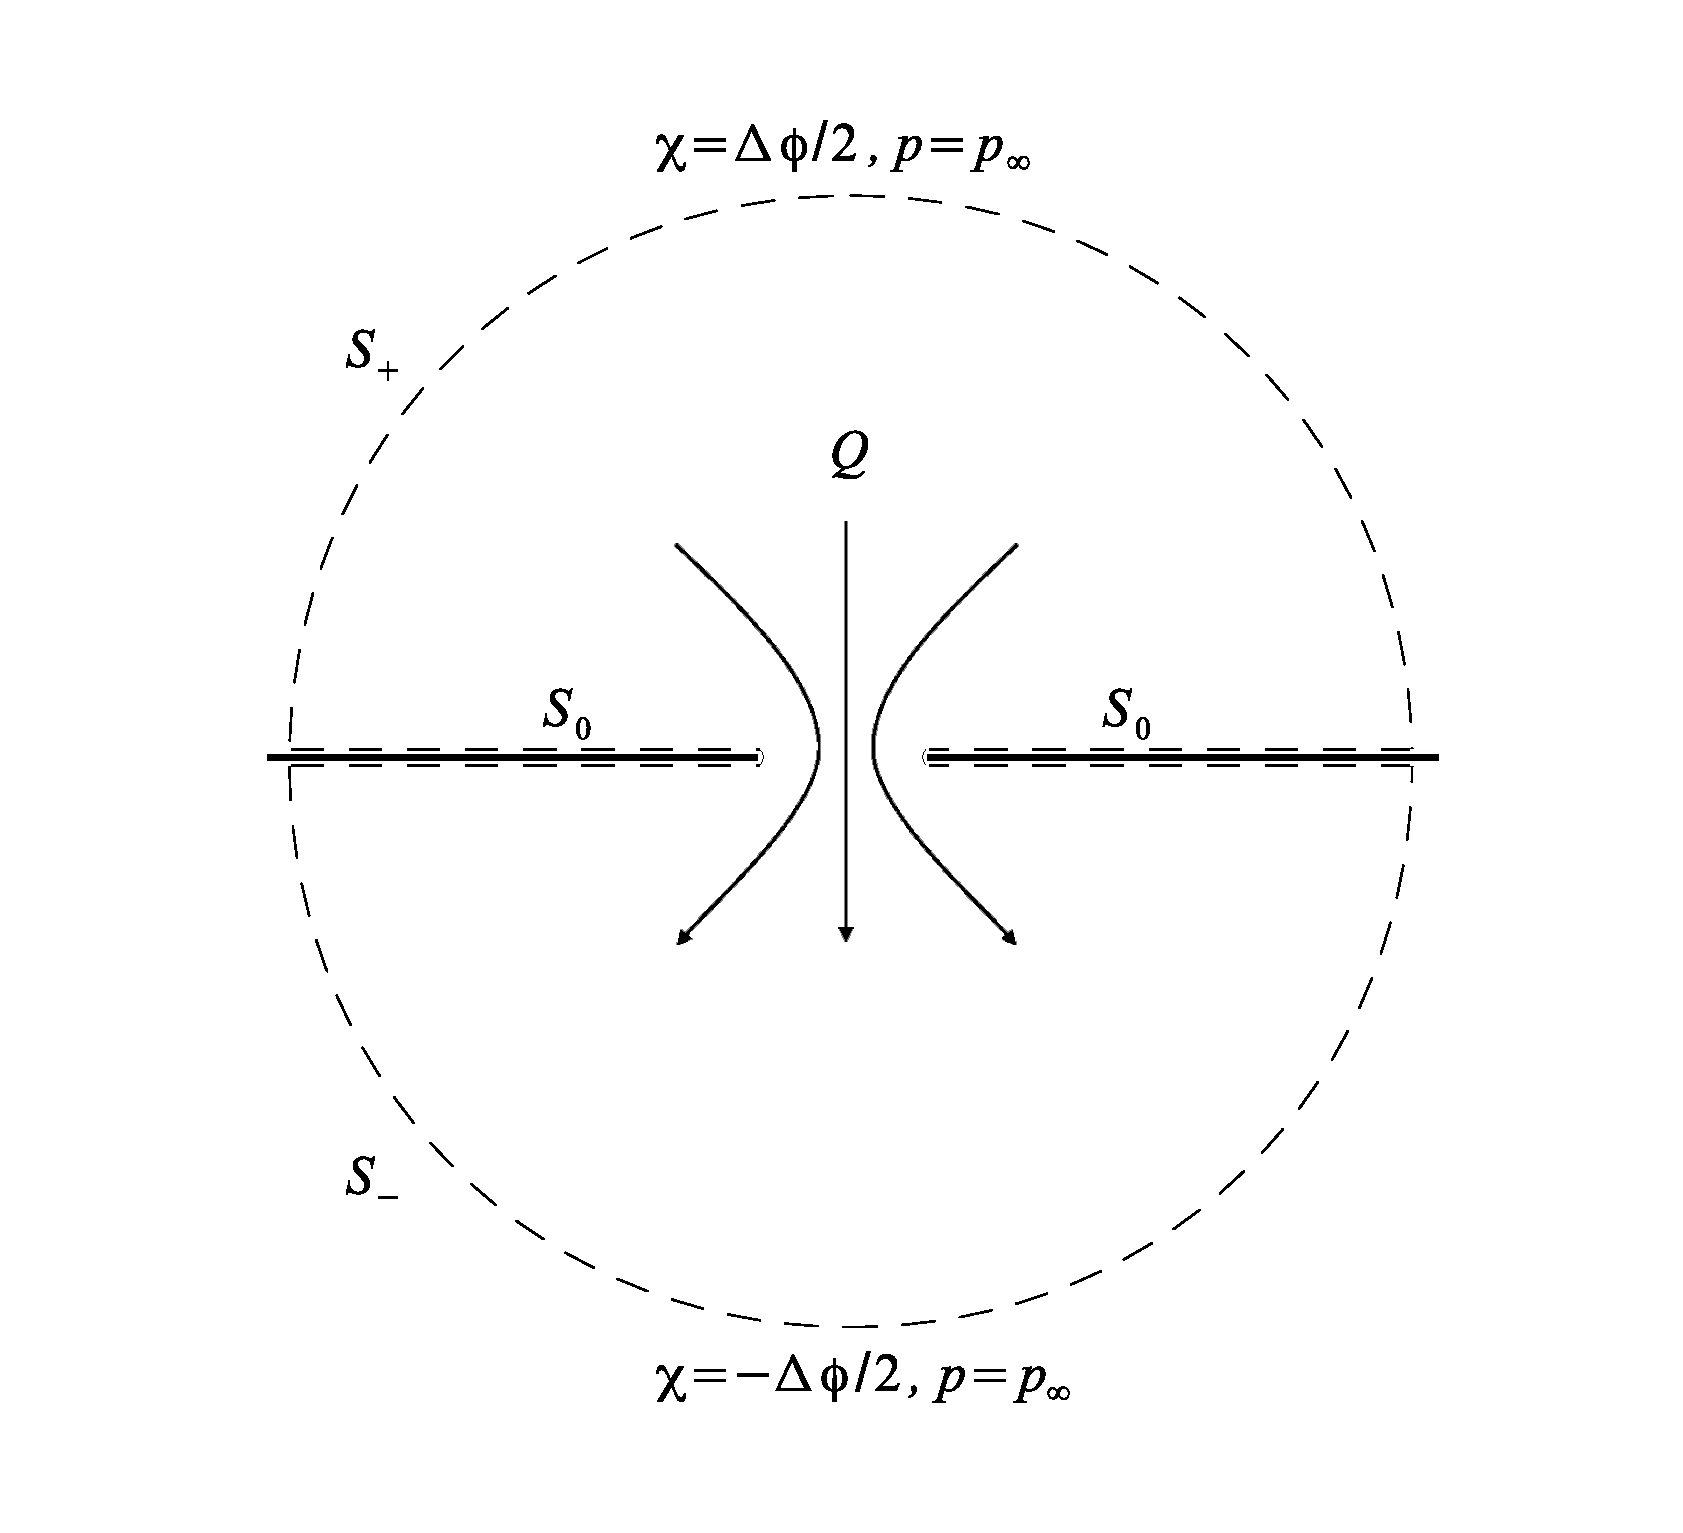
\includegraphics[width=0.8\textwidth]{zero_thickness/figure1.eps}
\caption{Flow through a charged membrane under an applied potential difference $\Delta\phi$.}
\label{fig:sketch}
\end{figure}
We consider a hole (of arbitrary shape) in an infinite plane membrane immersed in an incompressible homogeneous electrolyte containing $N$ ionic species (Figure~\ref{fig:sketch}). The number density of the $i$th ionic species is $n^i$, with $n^i=n_\infty^i$ in the bulk electrolyte far from any charged surfaces. The electrolyte has viscosity $\mu$ and electrical permittivity $\epsilon$. A surface charge of fixed density $\sigma$ exists at the membrane/electrolyte interface, and in the electrolyte adjacent to the membrane there is charge cloud of counter ions, with thickness characterized by the Debye length
\begin{equation}
\kappa^{-1}=\left(\frac{\epsilon k_BT}{\sum_{i=1}^N e^2 z_i^2n_\infty^i}\right)^{1/2},
\end{equation}
where $k_B$ is the Boltzmann constant, $T$ the absolute temperature, $e$ the proton charge, and $z_i$ the valence of the $i$th species of ion. We assume that the surface charge density $\sigma$ is sufficiently small so that the Poisson-Boltzmann equation describing the potential $\phi_0$ in the equilibrium charge cloud may be linearized. Far from any hole in the membrane, the zeta potential at the surface of the membrane is $\zeta=\sigma/(\epsilon\kappa)$,
with $\zeta\ll k_BT/e$. An electric potential difference $\Delta \phi$ is applied across the membrane with a resulting current $I$. The hole within the membrane has characteristic size $a$, and we make no assumption concerning $a\kappa$, the ratio of the hole size to the Debye length $\kappa^{-1}$. When $a\kappa\ll 1$, the charge clouds from opposite sides
of the perimeter of the hole overlap, but this has little effect upon the electrical conductivity of the hole when (as here) the surface charge density $\sigma$ and the resulting perturbations to the ionic number densities $n^i=n_\infty^i\exp(-ez_i\phi/k_BT)$ are small. Similarly, any ion exclusion effects of the overlapping charge cloud are negligible. We also note that the ion exclusion properties of a thin membrane are in general smaller than those of a long cylindrical pore. When $a\kappa\ll1$, the potential in the unperturbed electrical double layer within the pore, on the plane of the membrane, is $\zeta\approx\sigma/(\epsilon\kappa)$. Inside a uniform cylindrical pore with surface charge density $\sigma$, the potential when $a\kappa\ll 1$ is 
$\zeta\approx 2\sigma/(\epsilon a\kappa^2)$, and the condition $e\zeta/k_BT\ll 1$ required for the perturbation of the ionic number densities to be small within the pore implies a smaller charge density $\sigma$ for the pore than for the membrane. Only when $a\kappa=O(1)$ will the long cylindrical pore and the hole in a membrane exhibit similar ion exclusion properties.

When $a\kappa\gg 1$ the charge cloud is thin compared to the lateral dimension of the hole, but it remains thick compared to the membrane of zero thickness $h=0$ considered in \S~\ref{subsec:roundhole}. Thus, we are unable to appeal to Smoluchowski's analysis for thin charge clouds in \S~\ref{subsec:roundhole}. Ion exclusion effects are negligible in this limit.

In \S~\ref{subsec:charge_perturbation} we discuss how the charge cloud is deformed by the applied electric field and by fluid motion. We then (\S~\ref{subsec:formalism}) describe a theoretical framework for calculating the flow rate $Q$ through the hole, exploiting the reciprocal theorem: the analysis is similar to that of \cite{Sherwood1995}.  In \S~\ref{subsec:roundhole} we consider the special case of a circular hole in a thin membrane for which the integral for the flow rate $Q$ can be computed numerically.


\subsection{\label{subsec:charge_perturbation}The perturbed charge cloud}

When the electrical potential difference $\Delta\phi$ is applied across the membrane, the charge cloud adjacent to the surface of the membrane is perturbed, both by the direct electrical field $\nabla\phi$
acting on the ions, and by motion of the fluid. Ions are convected with the fluid velocity $\mathbf{u}$, and move relative to the fluid under the influence of electric fields and thermal diffusion.
The conservation equation for the number density $n^i$ of the $i$th ionic species, in steady state, is therefore
\begin{equation}
\nabla\cdot\left\lbrack n^i\mathbf{u} -\omega^i(k_BT\nabla
n^i + ez_in^i\nabla\phi) \right\rbrack=0 ,
\end{equation}
where $\omega^i$ is the mobility of the $i$th species of ion.

We follow \cite{saville1977} and nondimensionalise potentials by $k_BT/e$, lengths by the typical hole dimension $a$, velocities by $\epsilon(k_BT/e)^2/\mu a$ and mobilities by a characteristic mobility
value $\omega^0$. The equation in dimensionless form is then
\begin{equation}
\frac{\epsilon k_BT}{e^2\mu\omega^0}\nabla\cdot(\mathbf{u}n^i) = \nabla\cdot(\hat\omega^i\nabla n^i + z_i n^i \nabla \hat\phi)
\end{equation}

We assume that the potential $\Delta\phi$ which characterises the applied field is small compared to the equilibrium zeta potential $\zeta$, so that $\beta=e\Delta\phi/k_BT\ll e\zeta/k_BT$,
where $e\zeta/k_BT$ has already been assumed small in order that we may describe the charge cloud by means of the linearized Poisson-Boltzmann equation. We use the dimensionless field strength $\beta$ as the basis for a perturbation expansion:
\begin{subeqnarray}
\hat{\mathbf{u}} &=& \beta\hat{\mathbf{u}}_1 + \cdots\\
\hat\phi &=& \hat\phi_0 + \beta\hat\phi_1 +\cdots\\
n^i &=& n_0^i + \beta n_1^i + \cdots,
\end{subeqnarray}
where the subscript 0 refers to the equilibrium cloud, and the caret $\hat{ }$ denotes a nondimensional quantity.  

At $O(1)$ we get
\begin{equation}
\nabla(\hat\omega^i\nabla n^i + z_i n_0^i \nabla \hat\phi_0) = 0
\end{equation}
This is the Boltzmann distribution.

The steady-state ion conservation equation, correct to $O(\beta)$, becomes
\begin{equation}
\text{Pe} ~\hat{\mathbf{u}}_1\cdot\nabla n_0^i = \hat\omega^i\nabla\cdot\left\lbrack
 z_in_0^i\nabla\hat\phi_1 + z_in_1^i\nabla\hat\phi_0 +\nabla
n_1^i \right\rbrack
\label{convdiff}
\end{equation}
where the Peclet number $\text{Pe}=\epsilon k_BT/e^2\mu\omega^0$  characterizes the ratio of ionic convection to diffusion. Since the nondimensional equilibrium potential $\hat\phi_0$ has been assumed to be small, (\ref{convdiff}) reduces to
\begin{equation}
0 = z_in_\infty^i\nabla^2\hat\phi_1 + \nabla^2n_1^i . \label{eqn1}
\end{equation}
The boundary conditions at infinity are
\begin{subeqnarray}
n_1^i&\to&0,\\
\beta\phi_1&\sim&\pm\Delta\phi/2\hbox{\hskip 10pt in $z\gtrless 0$.}
\label{bc_infinity}
\end{subeqnarray}
This latter condition in \ref{bc_infinity} is equivalent to $\hat\phi_1 \approx \pm 1/2$ as $r \rightarrow \infty$ in $z\gtrless 0$.

We assume that no ions enter or leave the surface of the membrane. Hence
\begin{equation}
\mathbf{n}\cdot(k_BT\nabla n^i+ez_in^i\nabla\phi)=0,
\end{equation}
where $\mathbf{n}$ is the normal to the membrane. At $O(\beta)$, and assuming $\hat\phi_0\ll1$, this zero flux boundary condition becomes
\begin{equation}
\mathbf{n}.\nabla \left(n_1^i+z_in_\infty^i\hat\phi_1\right)=0 . \label{bc1}
\end{equation}

Multiplying Equation \ref{eqn1} by $e^2z_i$ and summing over $i$, we obtain, at $O(\beta)$,
\begin{equation}
\nabla^2\hat\chi_1=0,
\label{chieqn1}
\end{equation}
where
\begin{equation}
\hat\chi_1 = \hat\phi_1 + \hat\rho_1(a\kappa)^{-2},
\label{chieqn2}
\end{equation}
and
\begin{equation}
\hat\rho_1=\frac{ea^2\rho_1}{\epsilon k_BT}=\frac{ea^2}{\epsilon k_BT}\sum_{i=1}^N
ez_in_1^i
\end{equation}
is the (non-dimensional) perturbation to the charge density
$\rho=\sum_iez_in^i$.

The boundary conditions for (\ref{chieqn1}) are similarly obtained from
 (\ref{bc_infinity}) and (\ref{bc1}):
\begin{subeqnarray}
\hat\chi_1&\sim&\pm 1/2\quad
\hbox{as $\mathbf{r}\rightarrow\infty$ in $z\gtrless 0$,}
\\
\mathbf{n}\cdot\nabla\hat\chi_1&=&0\hskip 35pt\hbox{on the membrane,}
\label{chieqn3}
\slabel{chie_normal_bc}
\end{subeqnarray}
and we note that the boundary condition (\ref{chie_normal_bc}) represents zero flux of ions into the membrane, rather than a zero normal electric field. The potential
\begin{equation}
\chi=\phi_1+\rho_1/\epsilon\kappa^2
\end{equation}
is thus obtained by solving the Laplace equation for the potential created by applying the potential difference $\Delta\phi$ across the insulating membrane containing the pore. The potential $\chi$ is related to the linearized change
$\mu_1^i=ez_i\phi_1+k_BTn_1^i/n_\infty^i$ in the electrochemical potential of the $i$th species of ion, with $\chi=\sum_iez_in_\infty^i\mu_1^i/(\epsilon k_BT\kappa^2)$. As discussed by \cite{saville1977},
when $\hat\phi_0\ll 1$ the perturbation $\rho_1$ to the charge density
is negligibly small, so that $\phi_1=\chi$, and our analysis is equivalent to that of~\cite{Henry_1931}.


\subsection{A formalism for calculating the flow rate using the
reciprocal theorem}
\label{subsec:formalism}

The Stokes equations governing fluid motion are modified by the presence of an electric force $-\rho\nabla\phi$ acting on the fluid. Expanding in powers of $\beta$, we find
\begin{eqnarray}
\rho\nabla\phi&=&(\rho_0+\beta\rho_1)\nabla(\phi_0+\beta\phi_1)+O(\beta^2)
\nonumber\\
&=&-\nabla(\hbox{$\frac{1}{2}$}\epsilon\kappa^2\phi_0^2-\beta\rho_1\phi_0)
+\beta\rho_0\nabla(\phi_1+\rho_1/\epsilon\kappa^2)+O(\beta^2),
\label{rhophi}
\end{eqnarray}
where we have used the relation $\rho_0=-\epsilon\kappa^2\phi_0$ between the
equilibrium charge density $\rho_0$ and the equilibrium potential $\phi_0$ given by the linearized Poisson-Boltzmann equation. Hence the Stokes equations become
\begin{equation}
\mu\nabla^2\mathbf{u} -\nabla p - \rho_0\nabla\chi = 0,
\label{stokes}
\end{equation}
where the term $\nabla(\frac{1}{2}\epsilon\kappa^2\phi_0^2-\beta\rho_1\phi_0)$ in
(\ref{rhophi}) has been incorporated into the pressure $p$.

Note that the fluid motion caused by direct electrical forces acting on the fluid  create additional deformation of the charge cloud, but, as seen from Equation \ref{convdiff}, this deformation is $O({\hat u}_1 \text{Pe}\; \hat\phi_0)$, and may be neglected when
$\hat\phi_0$ is small. 

We now determine the $O(\beta)$ total volumetric flow rate $Q$ through the pore, created by the electrical force acting on the charge cloud within the fluid. Consider two Stokes flows $\mathbf{u}$ and $\bar{\mathbf{u}}$ in a volume $V$ with boundary conditions given on the bounding surface $S$
with outward normal $\mathbf{n}$. A body force $\mathbf{F}$ acts on the fluid, in which the pressure is $p$, the viscosity is $\mu$, the strain rate tensor is $e_{ij}=(\partial_iu_j+\partial_ju_i)/2$, and the stress tensor is $\tau_{ij}= - p \delta_{ij} + 2\mu e_{ij}$. Barred variables represent the corresponding quantities for the second flow $\bar{\mathbf{u}}$. The reciprocal theorem \cite{Happel&Brenner} gives the identity:
\begin{equation}
\int_V u_i \bar{F}_i dV + \int_S u_i \bar{\tau}_{ij} n_j dS = \int_V
\bar{u}_i F_i  dV + \int_S \bar{u}_i \tau_{ij} n_j dS.
\label{eq:recTheo}
\end{equation}

We suppose that flow 1 ($\mathbf{u}$)  is the flow of interest, namely, the electrokinetic flow through a hole in a charged membrane. The body force $\mathbf{F}$, by (\ref{stokes}), is
\begin{equation} 
\mathbf{F} = -\rho_0\nabla\chi,
\label{eq:forceF}
\end{equation} 
where, by (\ref{chieqn1}), $\nabla^2 \chi = 0$ with boundary conditions (\ref{chieqn3})
$\hat{\mathbf{n}} \cdot \nabla \chi = 0$ on the membrane surface $S_0$ and  $\chi \sim \pm \Delta \phi / 2$ on surfaces $S_{\pm}$ far from the pore (Figure~\ref{fig:sketch}).

We take flow 2 ($\bar{\mathbf{u}}$) to be that due to a pressure difference $\Delta p$ imposed across a pore in an uncharged membrane; thus, the body force $\bar{\mathbf{F}}=0$. Since the Stokes flow equations are linear, we may write 
\begin{equation} 
\bar{\mathbf{u}} = \Delta p\, \mathbf{G},
\label{eq:defineG}
\end{equation} 
where $\mathbf{G}$ is a function that depends solely on the pore geometry. 

We now substitute the two flows into the reciprocal relation (\ref{eq:recTheo}). The bounding surface $S$ is as shown in Figure~\ref{fig:sketch}; it consists of two hemispheres $S_{+}$ and $S_{-}$ of very large radius $R$, together with the membrane surface, $S_{0}$.
On $S_{0}$, the velocities $u_{i}, \bar{u}_{i}=0$ whereas on 
$S_{\pm}$ we have $\tau_{ij} \sim - p_{\pm} \delta_{ij} + O(R^{-3})$ and 
$\bar{\tau}_{ij} \sim - \bar{p}_{\pm} \delta_{ij} + O(R^{-3})$ where $p_{\pm}$ are the pressures 
at great distance $R$ from the pore on either side of the membrane. 
For flow 1, $p_{+}=p_{-} = p_{\infty}$ and for flow 2, $\bar{p}_{+} - \bar{p}_{-} = \Delta p$. Substituting
(\ref{eq:forceF}) and (\ref{eq:defineG}) into (\ref{eq:recTheo}), and cancelling the pressure difference $\Delta p$ from both sides of the equation, we obtain
\begin{equation}
Q = \int_{S_-}\mathbf{u}\cdot\mathbf{n}\; dS=
 - \int_{S_+}\mathbf{u}\cdot\mathbf{n}\; dS =
- \int_V \rho_0 \mathbf{G} \cdot \nabla \chi \; dV,
\label{eq:Q1}
\end{equation}
where $Q$ is the volumetric flux of flow 1 from the side $S_{+}$ to the side $S_{-}$ of the 
membrane.


\subsection{Flow rate from a round hole in elliptic cylindrical co-ordinates}\label{subsec:roundhole}
We now consider a circular pore of radius $a$. We adopt cylindrical co-ordinates  $(r,z)$, with origin at the centre of the pore and $z$ along the axis of symmetry, together with oblate spherical coordinates $(\xi,\eta)$ where $\infty > \xi > - \infty$, $\pi/2 > \eta \geq 0$ such that
\begin{equation}
z=a\sinh\xi\cos\eta\quad,\quad r=a\cosh\xi\sin\eta.
\end{equation}
The scale factors are
\begin{equation}
h_\xi=h_\eta=a(\cosh^2\xi-\sin^2\eta)^{1/2}.
\end{equation}
The imposed electric field is given by  \cite[p. 1292]{M&F}, with potential
\begin{equation}
\chi = \frac{\Delta \phi}{2} \left[ 1- \frac{2}{\pi}
\tan^{-1}\left( \frac{1}{\sinh \xi} \right) \right].
\label{eq:chi}
\end{equation}
\cite[p. 153]{Happel&Brenner}
give the stream function $\psi=-a^3\Delta p(1-\cos^2\eta)/(6\pi\mu)$ for
flow 2. Comparing the resulting velocity, $\bar{\mathbf{u}}$, with
(\ref{eq:defineG}),
\begin{equation}
G_\xi =  - \frac{a \cos^2\eta}{2\pi\mu
\cosh\xi(\cosh^2\xi-\sin^2\eta)^{1/2}}\quad,\quad
G_\eta  =  0.
\label{eq:u2}
\end{equation}
Substituting (\ref{eq:chi}) and (\ref{eq:u2}) into (\ref{eq:Q1}) yields the electroosmotic flow rate
\begin{equation}
Q   =  \frac{2a^3\Delta\phi}{\pi\mu}
\int_0^{\frac{\pi}{2}} d\eta \int_0^\infty \rho_0
\frac{\cos^2\eta\sin\eta}{\cosh\xi} d\xi.
\label{eq:Q2}
\end{equation}
Detailed derivations of Equation \ref{eq:Q2} are given in Appendix.

The equilibrium charge density $\rho_0$ in the linearized, Debye H\"{u}ckel limit may be obtained by excising the solution for a uniformly charged disk  \cite{Sherwood1995} from that for a charged infinite plate. 
Hence
\begin{eqnarray}
\rho_0 & = & \sigma  \kappa^2 a \left[  \int_0^\infty
\frac{J_1(as)J_0(rs)}{(\kappa^2+s^2)^{1/2}}
e^{-(\kappa^2+s^2)^{1/2} z} ds - \frac{e^{-\kappa z}}{\kappa a} \right].
\label{eq:rho0}
\end{eqnarray}

The integral in (\ref{eq:Q2}) cannot be evaluated in closed form when $\rho_0$ is given by (\ref{eq:rho0}). However, in the long Debye length limit  $\kappa a \ll 1$, the rate of decay of $\mathbf{G}$ and $\nabla \chi$ is such that the major contribution to the integral (\ref{eq:Q2}) comes from a region (near the hole) of volume $O(a^3)$, within which $\rho_0 \approx -\sigma\kappa$. Thus,
\begin{equation}
Q \sim - \frac{2a^3\Delta\phi}{\pi\mu} (\sigma \kappa)
\int_0^{\pi/2} \cos^2\eta \sin\eta \, d\eta \int_0^\infty
\frac{d\xi}{\cosh\xi} = - \frac{a^3\kappa\sigma\Delta\phi}{3\mu} = \kappa a Q_{0},
\label{eq:QaKappaSmall}
\end{equation}
where $Q_{0}= - a^2 \sigma\Delta\phi/ (3\mu)$ is a convenient characteristic flow rate.

In other cases, the integral must be evaluated numerically. It is convenient to introduce new variables 
$x=\kappa a$, $t=sa$, $\bar{r} = r/a$, $\bar{z} = z/a$ in terms of which (\ref{eq:rho0}) becomes
\begin{equation}
\rho_0 = \sigma\kappa^2 a \left(I_1 - \frac{e^{-x\bar{z}}}{x} \right)
\label{eq:rho0_modified}
\end{equation}
and (\ref{eq:Q2}) becomes 
\begin{equation}
Q = \frac{2a^2 \sigma \Delta\phi}{\mu\pi} \left[ - x
I_2 + x^2 \int_0^{\pi/2} d\eta \int_0^\infty I_1
\frac{\cos^2\eta\sin\eta}{\cosh\xi} d\xi \right],
\label{eq:Q3}
\end{equation}
with $I_1$ and $I_2$ defined as 
\begin{eqnarray} 
I_1 &=& \int_0^\infty
\frac{J_1(t)J_0(\bar{r}t)}{\sqrt{x^2+t^2}}
\exp[ - \bar{z} \sqrt{x^2+t^2}   ] dt, 
\label{eq:I1_define}
\\ 
I_2 &=& \int_0^{\pi/2}d\eta \int_0^\infty e^{-x\sinh\xi\cos\eta} \frac{\cos^2\eta\sin\eta}{\cosh\xi} d\xi \nonumber \\
    &\overset{\cos\eta\rightarrow q}{=}&  \int_0^1 q^2 \left[
ci(x q)\sin(x q )- si(x q )\cos(x q) \right] d q,
\label{eq:expTermInt}
\end{eqnarray}
where $si(\alpha), ci(\alpha)$ are the sine and cosine integrals 
\begin{equation}
si(\alpha) = - \int_\alpha^\infty \frac{\sin t}{t}\, dt\quad , \quad
ci(\alpha) = -\int_\alpha^\infty \frac{\cos t}{t}\,dt.
\end{equation}

The integrals $I_1$ (\ref{eq:I1_define}) and $I_2$ (\ref{eq:expTermInt}) were evaluated using the Matlab routine \textbf{quadgk} \cite{matlab}. $I_1$ represents the potential due to a thin charged disk,
and decays exponentially at large distances, as does $1/\cosh(\xi)$. The $\xi$ integration in
(\ref{eq:Q3}) could therefore be truncated at a large value, taken to be $\xi=8$
(corresponding to a distance $\approx 1490a$ from the pore). To evaluate the second term in brackets in (\ref{eq:Q3}), the $(\xi,\eta)$ space was divided into sub-regions, with typically 500 intervals for $\xi$ and 200 for $\eta$. Smaller intervals were used near the pore ($\xi\ll 1$) and near
the membrane ($\pi/2-\eta\ll 1$). For every pair $(\xi,\eta)$, the integral $I_1(\xi,\eta)$ was numerically
evaluated using Matlab routine and $Q$ was obtained via trapezoidal summation again within Matlab. Results are shown in Figure~\ref{fig:QaKappa} with the asymptotic regime $\kappa a \ll 1$, described by (\ref{eq:QaKappaSmall}), depicted by the dashed straight line of unit slope. 

\begin{figure}[h]
\centering
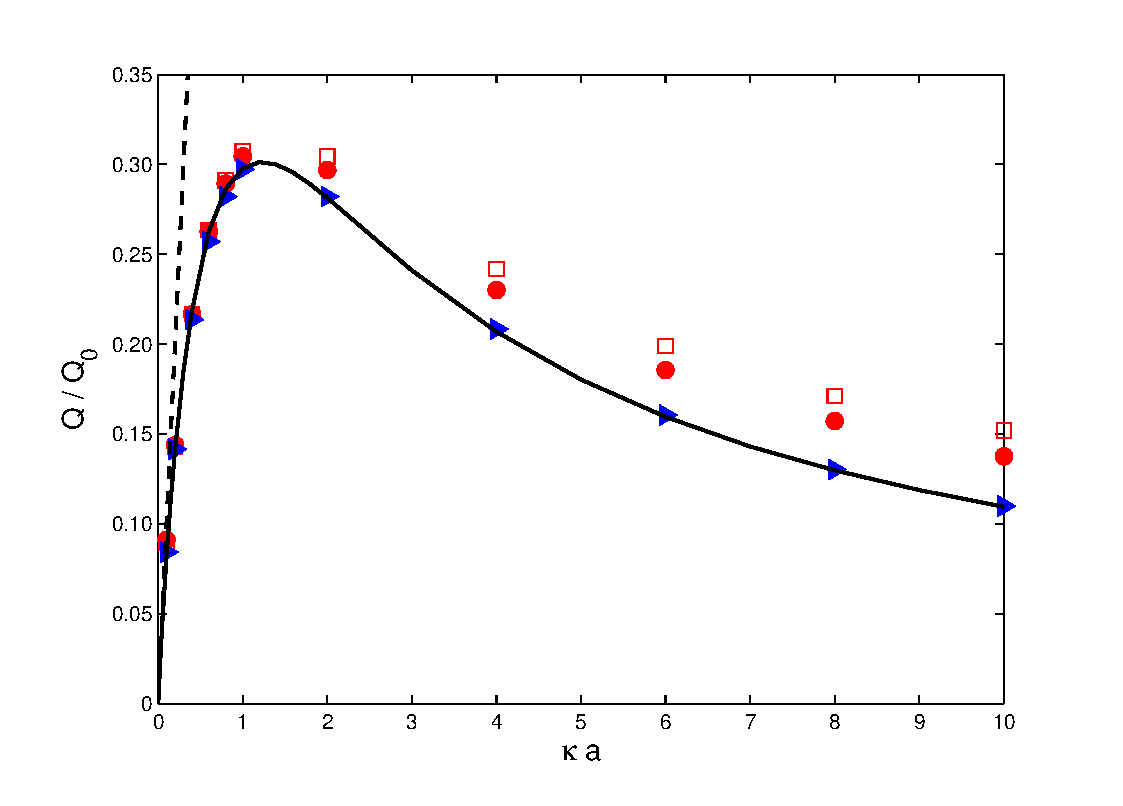
\includegraphics[width = 0.8\textwidth]{zero_thickness/figure2.eps}
\caption{The normalized flow rate $Q/Q_0$ through a circular pore of radius $a$ 
in a membrane of thickness $h=0$ as a function of $\kappa a$ determined from (\ref{eq:Q3})  (solid line), with asymptote $Q/Q_{0} \sim \kappa a$ (\ref{eq:QaKappaSmall}) (dashed line). The symbols are from the full finite volume simulations of \S~\ref{sec:fullSim} with $h/a=$ 0 (triangle), 0.06 (circle) 
and 0.1 (square).}
\label{fig:QaKappa}
\end{figure}

\section{Flow through a hole in a membrane of finite thickness}
\label{sec:fullSim}
In order to examine the validity of (\ref{eq:Q3}), the full Poisson-Nernst-Planck-Stokes system of equations in Chapter \ref{chpt:intro} are solved numerically using a finite volume method based on the open source CFD library OpenFOAM \cite{OPENFOAM}. Our numerical model has been described by \cite{Mao2013} and details of the implementation for the current problem will be presented in \S~\ref{sec:numerical}. The cases studied include membranes of thickness $h=0$ and $h>0$ in the regime of weak applied fields and low membrane charge. These conditions, stated in \S~\ref{subsec:formalism}, may be restated more conveniently as $ \hat{\phi}^{-1} \gg \kappa a \gg \hat{\sigma}$ where $\hat{\sigma} = a e |\sigma| / (\epsilon k_BT)$ and $\hat{\phi} = |\epsilon\Delta \phi / (\sigma a)|$ are dimensionless parameters characterizing the degree of membrane charge and the strength of the applied field respectively. In the simulations presented here, the values of these parameters were $\hat{\sigma} = 0.273$ and $\hat{\phi}=0.071$ so that (\ref{eq:Q3}) can be expected to be a reasonable approximation in the range $14 \gg \kappa a \gg 0.3$. 

The computed flow rate $Q$ normalized by $Q_{0} =  - a^2 \sigma\Delta\phi/(3\mu)$ is shown 
by the symbols in Figure~\ref{fig:QaKappa}. Good agreement with (\ref{eq:Q3}) is obtained, but  
thicker membranes result in somewhat increased flow rates. The discrepancy increases at 
shorter Debye lengths.  

The analysis of \S~\ref{sec:zeroThick} assumed that effects due to induced charge electroosmosis (ICEO) are negligible. However, \cite{Thamida2002} have shown that ICEO generates vortices at sharp corners, and such
vortices will inevitably be generated in the membrane geometry considered here. In the vicinity of the edge of the nanopore, where $r/a=1+s$, the potential $\chi$ (\ref{eq:chi}) on the membrane surface
$z=0$ may be expanded as
\begin{equation}
\chi=\pm\frac{\Delta\phi}{\pi}\sqrt{2s},\quad \hbox{on $z=\pm0$.}
\end{equation}
If we assume that this potential is little modified when the membrane has a finite thickness $h>0$, the potential gradient within the solid membrane due to the external potential $\chi$ is
\begin{equation}
\frac{\partial\phi_s}{\partial z}=\frac{2\Delta\phi}{\pi}\frac{\sqrt{2s}}{h},
\end{equation}
and if $\epsilon_s\ll\epsilon$ the induced potential gradient normal to the surface within the liquid is 
$(\epsilon_s/\epsilon)\partial\phi_s/\partial z$. This corresponds to an induced surface charge (with accompanying charge cloud of couter-ions)
\begin{equation}
\sigma_i=\mp\frac{2\epsilon_s\Delta\phi}{\pi}\frac{\sqrt{2s}}{h}
,\quad \hbox{on $z=\pm0$.}
\label{induced_charge}
\end{equation}
The analysis breaks down when $s \lesssim h/a$ where the detailed geometry near the edge of the pore becomes important. If the membrane has rounded edges, the curvature $\sim h^{-1}$ and the induced charge is at most $\sigma_{i} \sim \epsilon_s\Delta\phi/(ah)^{1/2}$. This may be neglected as long as it is small compared to $\sigma$, or equivalently, if $(\epsilon_s/\epsilon) \sqrt{(a/h)} \; \hat{\phi} \ll 1$.
For common membrane materials (e.g. lipids and silica) $\epsilon_s / \epsilon \sim 0.1$, thus, 
as long as the applied field remains weak, ICEO effects are restricted to the neighbourhood of
sharp corners.

The results of full numerical solutions of the Poisson-Nernst-Planck-Stokes equations reported in Figure~\ref{fig:QaKappa} were computed with membrane permittivity $\epsilon_s=0$.
However, it is shown in \S~\ref{sec:numerical} that numerical solutions for appropriate non-zero solid permittivities $\epsilon_s >0$ predict flow rates $Q$ that differ little from those with $\epsilon_s=0$
in the parameter regime under consideration. The contribution of such effects to the net fluid flux, $Q$,
is at best very weak. This is perhaps not surprising, since even when (as here) there are sharp corners, if the membrane is uncharged and the electrolyte is symmetric (with identical ionic mobilities),
symmetry dictates that ICEO cannot generate a net flow $Q$ through the pore. So although nonlinear
effects such as ICEO can generate a net fluid flow through a charged membrane, the applied field $\Delta\phi$ must be larger than the fields considered here. An ICEO contribution to the fluid flux is in principle possible, but only for a charged membrane at high applied fields, as, for example, in the numerical results presented by \cite{Mao2013}.

The reciprocal theorem used in \S~\ref{subsec:formalism} enabled
us to determine the volumetric flow rate $Q$ through the pore without a full computation of the velocity field. This has the advantage of leading quickly to a value for $Q$. However, this approach hides other interesting features of the flow, such as eddies, whether generated by ICEO \cite{Thamida2002} or by the pore throat restricting the flow \cite{park2006eddies}. These features are only revealed by full numerical computations, such as those discussed in \S~\ref{sec:numerical}.


\subsection{The limits of thick and thin membranes} 
Since the fluid flux through the pore is generated by the applied potential, $\Delta \phi$,
we can define an ``electroosmotic conductance'' $H = Q/\Delta\phi$ in analogy to the electric conductance. If the membrane thickness  $h \gg a$, we have a long cylindrical pore with surface charge density $\sigma$ at the wall. 
%Within the channel, 
The electroosmotic flow velocity is then \cite{levine1975}
\begin{equation}
u = \frac{\epsilon E_0}{\mu} [\phi_0 - \zeta]
\label{eq:axial_velocity_u}
\end{equation} 
where $\phi_0=-\epsilon\kappa^2\rho_0$ is the equilibrium potential in the double layer, $\zeta$ is the equilibrium potential at the wall, and $E_0 = \Delta\phi / h$. The equilibrium potential of a cylindrical pore in the Debye-H\"{u}ckel limit is
\begin{equation}
\phi_0 = \zeta \frac{I_0(\kappa r)}{I_0(\kappa a)}
= \frac{\sigma}{\epsilon\kappa} \frac{I_0(\kappa r)}{I_1(\kappa a)}.
\end{equation} 

Integrating the fluid velocity $u$ (\ref{eq:axial_velocity_u}) over the cross-section we obtain the volumetric flow rate $Q$ and hence the the electroosmotic conductance \cite{rice1965}
\begin{equation}
H_c = \frac{Q}{\Delta\phi} = \frac{2\pi\sigma a^3}{\mu h} \left[
\frac{1}{(\kappa a)^2} - \frac{1}{2(\kappa a)} \frac{I_0(\kappa
a)}{I_1(\kappa a)} \right].
\label{eq:Hc}
\end{equation}

On the other hand, when the thickness $h/a \ll  1$, we expect the system to be identical to a hole in a zero-thickness membrane, and the electroosmotic conductance may be obtained using (\ref{eq:Q3}):
\begin{equation}
H_p = \frac{Q}{\Delta\phi} =
\frac{2 \sigma a^2}{\mu\pi} \left[ - (\kappa a)
I_2 + (\kappa a)^2 \int_0^{\pi/2} d\eta \int_0^\infty I_1
\frac{\cos^2\eta\sin\eta}{\cosh\xi} d\xi \right].
\label{eq:Hp}
\end{equation} 

\subsection{The electroosmotic access resistance of a nanopore}
If a membrane of thickness $h$ containing a circular hole of radius $a$ separates two uniformly conducting regions, then the electrical resistance of the cylindrical hole increases,
proportional to $h$. This might suggest a vanishing resistance for an infinitely thin membrane. However, in reality, as $h\rightarrow 0$ the electrical resistance is dominated by entrance and exit effects,
and can be determined from the electrical potential (\ref{eq:chi}). This is called the ``access resistance'' of the pore and for a circular pore in an infinitely thin membrane it is described by a simple analytical formula \cite{Hall1975}.

An analogous situation applies to the problem of electroosmotic flow through a pore in a membrane. When the pore length $h$ is large compared to the pore radius $a$, the flow conductance $H \sim H_c \sim h^{-1}$ from (\ref{eq:Hc}) - a consequence of the fact that the electric field in the pore, $E \sim \Delta \phi / h$. However, $H$ does not increase indefinitely as $h \rightarrow 0$ but instead approaches a finite value $H_p$ given by (\ref{eq:Hp}). The surface charge $2\pi ah\sigma$ within the cylindrical pore goes to zero as $h\rightarrow 0$. Electroosmotic motion is therefore determined by
flow in the fluid on either side of the membrane, as described in \S~\ref{sec:zeroThick}, and not by the cylindrical pore. Thus, in analogy to the corresponding electrical problem, $H_p^{-1}$ may be regarded as an  ``access resistance'' of the pore to electroosmotic flow.

Figure~\ref{fig:flowConduc} shows the electroosmotic conductance $H$ obtained from 
the finite volume numerical computations as a function of  $h/a$. The computed value of $H$ is normalized by $H_p$ obtained from (\ref{eq:Hp}). It is seen that $H/H_p$ approaches unity as $h/a \rightarrow 0$ and approaches $H_c/H_p \sim h^{-1}$ for large $h/a$. The dashed line representing $H_c/H_p$ was obtained from (\ref{eq:Hc}) and (\ref{eq:Hp}). The results of the full computations indicate that though $H$ does exhibit the expected limiting behaviors, it does not vary monotonically with $h$ at short Debye lengths. The origin of the peak at intermediate values of $h/a$ will be investigated further in future work.

\begin{figure}[h]
\centering
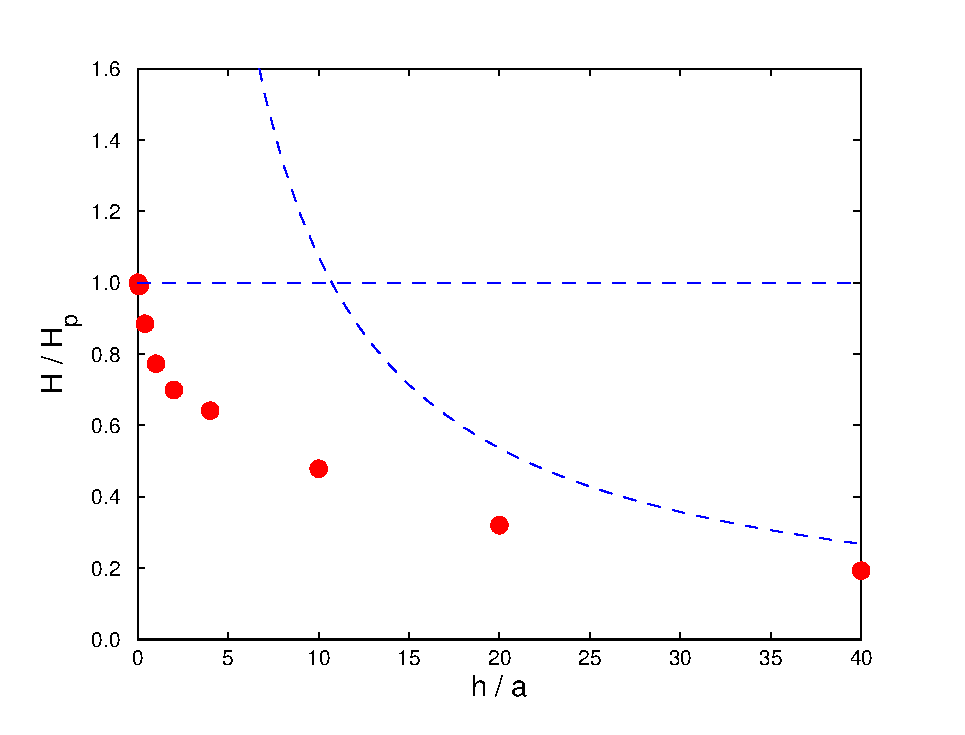
\includegraphics[width=0.45\textwidth]{zero_thickness/figure3a.eps}
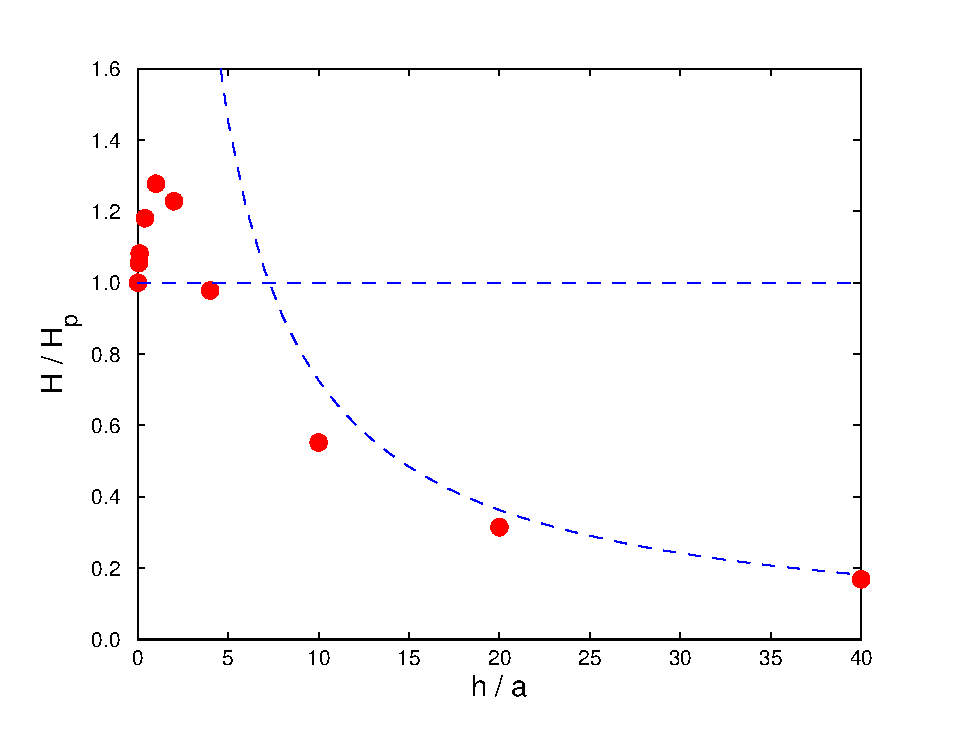
\includegraphics[width=0.45\textwidth]{zero_thickness/figure3b.eps}
\caption{The normalized ``electroosmotic conductance'' $H/H_p$ determined from the full 
numerical simulation (symbols) as a function of the normalized membrane thickness, $h/a$. Left panel corresponds to $\kappa a = 0.4$ and right panel $\kappa a = 2.0$.
The dashed lines correspond to the thin ($H=H_p$) and thick 
($H=H_c$) membrane limits obtained from (\ref{eq:Hc}) and (\ref{eq:Hp}).}
\label{fig:flowConduc}
\end{figure}

\section{Numerical solution of the PNP-Stokes equations}\label{sec:numerical}
\subsection{Numerical scheme}
An electrohydrodynamic solver was developed to solve the Poisson-Nernst-Planck-Stokes (PNP-Stokes) system of equations using the finite volume method. The solver was based on the OpenFOAM CFD library \cite{OPENFOAM}, a C++ library designed for computational mechanics,
containing a collection of object-oriented classes developed to represent mesh, fields, matrices and the necessary operations on fields and tensors. It also provides functions to handle finite volume discretization and matrix equation solving. 

The time-independent PNP-Stokes equations are rewritten here:
\begin{eqnarray}
\epsilon \nabla^2 \phi + \sum_{i=1}^{N} z_ien^i & = & 0,
\label{eq:poisson1}
\\
\nabla\cdot\left\lbrack n^i\mathbf{u} -\omega^i(kT\nabla
n^i + ez_in^i\nabla\phi) \right\rbrack&=&0 ,
\label{eq:NP1}
\\ 
-\nabla p + \mu \nabla^2 \mathbf{u} -  \nabla \phi \sum_{i=1}^{N} z_ien^i & = & 0, \label{eq:stokes1}\\
\nabla \cdot \mathbf{u} & = & 0. \label{eq:continuity1}
\end{eqnarray} 

In our simulation we consider a 1-1 symmetric electrolyte solution containing ions with equal mobilities. The boundary conditions to be satisfied by the solution are discussed in \S~\ref{sec:math_model}.

We apply the following scheme to solve the PNP-Stokes equations. We start from a zero flow field. Equations \ref{eq:poisson1} and \ref{eq:NP1} are solved sequentially in a loop with under-relaxation until the absolute residual is smaller than $10^{-6}$. Under-relaxation is necessary because the PNP system is non-linear. The electric volume force $- \nabla \phi\sum_i z_ien^i $ is obtained from this solution and used explicitly in the next step: the solution of the incompressible Stokes flow: (\ref{eq:stokes1}) and (\ref{eq:continuity1}). The SIMPLE algorithm is used with a fixed volume force density. The flow field is then substituted into (\ref{eq:NP1}). The PNP equations are then solved again using the updated flow field. An outer loop is constructed to iterate over the PNP loop and Stokes flow module.

For the finite volume discretization of the governing equations, central differences are used for all diffusive terms in (\ref{eq:NP1}) and viscous terms in (\ref{eq:stokes1}). A second-order upwind scheme is used for the convective terms in (\ref{eq:NP1}). The discretized linear system is solved using a pre-conditioned conjugate gradient solver if the matrix is symmetric or a pre-conditioned bi-conjugate gradient solver if the matrix is asymmetric. The details of the numerical algorithm are given by \cite{ferziger&peric}. 

\subsection{Mathematical model of the nanopore}\label{sec:math_model}
\begin{figure}[h]
\centering
\includegraphics[width=1.0\textwidth]{zero_thickness/figure4.eps}
\caption{A sketch of the axisymmetric geometry used in the simulation.}
\label{fig:system}
\end{figure}
A schematic view of the axisymmetric geometry used for the full numerical
simulations is provided in Figure~\ref{fig:system}. It consists of a circular hole of radius $a$ in a solid dielectric membrane CDEF of arbitrary thickness $h\ge 0$. The membrane surfaces CD, DE and EF have a uniform surface charge density $\sigma$. Two large cylindrical reservoirs are connected to the pore, one at each end. The length and radius of both the reservoirs are identical, and are
$L_R=\max(10a, 10\kappa^{-1})$, chosen to be much larger than either the hole radius $a$ or the Debye length $\kappa^{-1}$  in order to approximate an infinite reservoir. 


We adopt the following boundary conditions \cite{Mao2013}. The ion number densities on AB and GH are constant, and equal to the number density $n_\infty$ in the bulk solution far from any charged surfaces. The electrical potentials are uniform on AB and on GH, with a potential difference of $\Delta\phi$ between the top (AB) and bottom (GH). The pressure $p_{\infty}$ on AB is uniform and equal to that on GH. On the side walls BC and FG, the radial electric field, ionic flux and radial velocity, which decay away from the pore, are set to zero. A zero tangential shear stress is imposed on flow parallel to the side walls. At the membrane surfaces CD, DE and EF, a no-flux condition is used for 
(\ref{eq:NP1}), a no-slip condition for the flow; the electric field $\mathbf{E}$ undergoes a jump across the solid-fluid interface such that
$\epsilon \mathbf{E} \cdot  \hat{\mathbf{n}} - \epsilon_{s} \mathbf{E}_{s} \cdot \hat{\mathbf{n}} = \sigma$ 
where $\epsilon$ is the electrical permittivity of the
fluid and $\epsilon_{s}$ is the permittivity of the membrane, $\mathbf{E}_{s}$ is the electric field 
at the interface within the membrane and $\hat{\mathbf{n}}$ is the unit normal at the surface directed 
into the fluid. The potential is continuous across the interface. 

The strength of the applied field and the amount of surface charge can be characterized 
by the dimensionless parameters $\hat{\phi} = |\epsilon \Delta \phi/(\sigma a)|$ and 
$\hat{\sigma} = a e |\sigma | / (\epsilon kT)$ respectively. In the simulations presented here, 
the values of these parameters were kept fixed at $\hat{\phi}=0.071$ and $\hat{\sigma} = 0.273$.
The flow rate $Q$ was obtained by numerically integrating the $z$-component of the velocity over the plane $z=0$.

\subsection{Effect of membrane polarizability}
If the membrane polarizability is sufficiently small that
$|\epsilon_{s} \mathbf{E}_{s} \cdot \hat{\mathbf{n}}|\ll|\epsilon \mathbf{E} \cdot  \hat{\mathbf{n}}|$, then the jump condition of the normal component of the field may be replaced by
 $\epsilon \mathbf{E} \cdot \hat{\mathbf{n}} = \sigma$. 
In this case, the computational domain may be restricted to include only the fluid phase. This approximation was adopted for the results presented in Figures~\ref{fig:QaKappa} and
\ref{fig:flowConduc}.
Thus, effects due to Induced Charge Electroosmosis (ICEO) were neglected. 
The results of a calculation to test the validity of this assumption in the parameter range 
of interest are shown in Figure~\ref{fig:QaKappaEpw0}. The data from Figure~\ref{fig:QaKappa} for a non-polarizable membrane of thickness $h = 0.1a$ are reproduced in Figure~\ref{fig:QaKappaEpw0}. 
 For comparison, the result of a second calculation in which the dielectric constant of 
the membrane material was set to $3.9$ (corresponding to silica) is also shown. The electrolyte 
is considered polarizable with a dielectric constant of $80$. It is seen that 
the effect of membrane polarizability on the flow rate is negligible.

\begin{figure}[h]
\centering
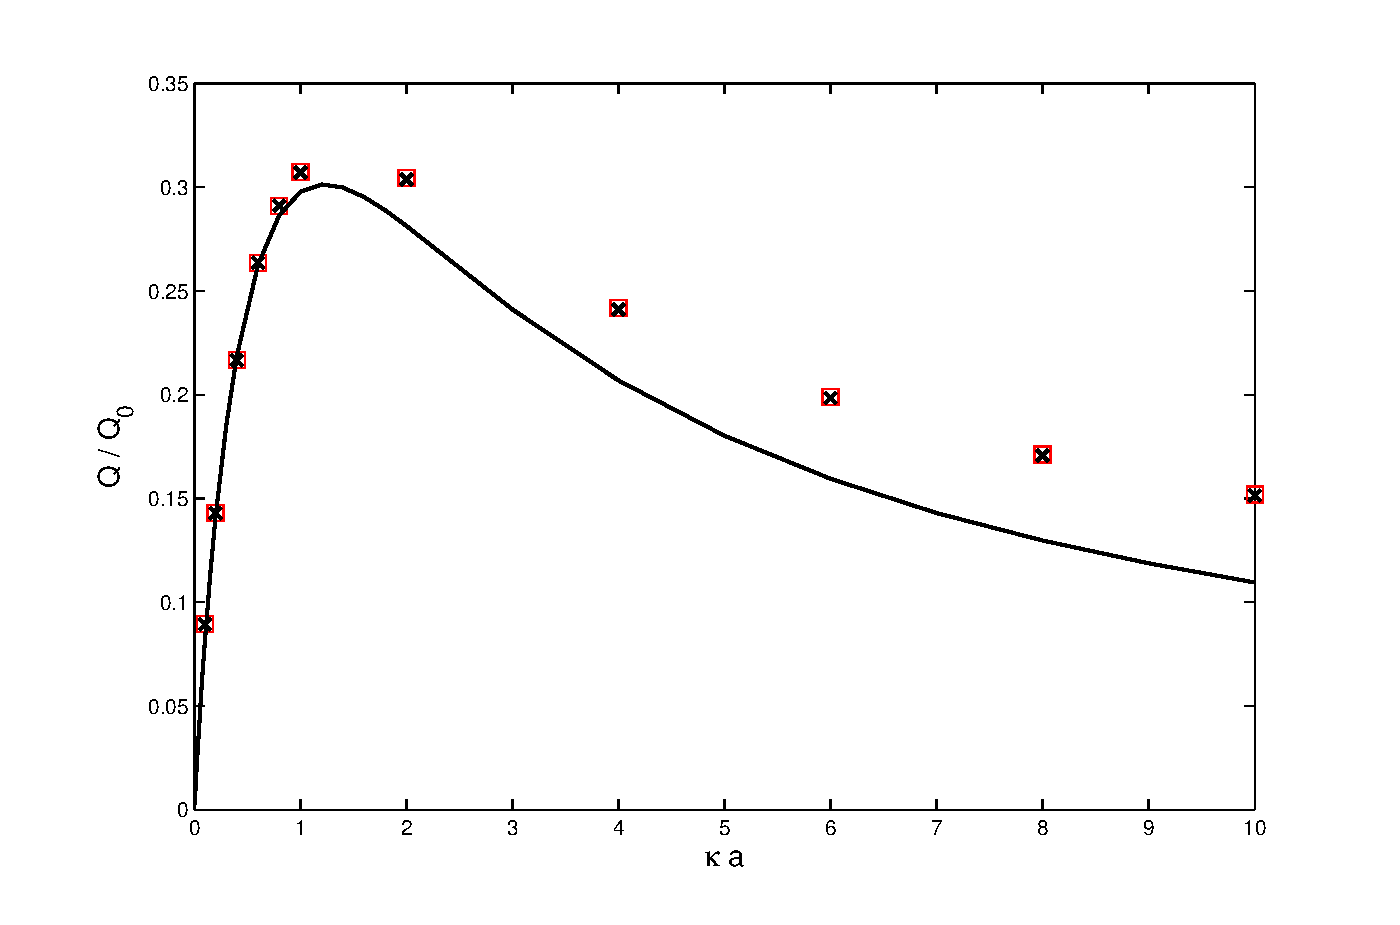
\includegraphics[width = 1.0\textwidth]{zero_thickness/figure5.eps}
\caption{The normalized flow rate through a circular pore of radius $a$ in a thin membrane 
as a function of $\kappa a$. The solid line shows results for a membrane of zero thickness,
obtained via the reciprocal theorem and (\ref{eq:Q2}).
The symbols are from the full numerical simulation with a membrane
of thickness $h = 0.1a$.
Squares show results for
 a non-polarizable membrane $\epsilon_s=0$, crosses show results for 
 a membrane with a dielectric constant $3.9$. The  dielectric constant of 
 the electrolyte is $80$. The effect on the flow rate
due to membrane polarizability and consequent ICEO
 is seen to be negligible.}
\label{fig:QaKappaEpw0}
\end{figure}

\section{Concluding Remarks}\label{sec:conclusion}
We have assumed that the surface charge density $\sigma$ is sufficiently low 
% so 
that the zeta potential is small, $\zeta\ll k_BT/e\approx 25\rm\ mV$ at $T=298\rm\ K$.
Thus, the Poisson-Boltzmann equation can be linearized.
%and the Poisson-Boltzmann equation can be linearized, with $\zeta\ll k_BT/e\approx 25\rm\ mV$ at $T=298\rm\ K$. 
Non-dimensional zeta potentials $e\zeta/k_BT$ in colloidal systems, though not always small, are typically at most 5, and it is found that theories based on small potentials usually give useful
qualitative insight into electrokinetic behaviour over this range of potentials (e.g. \cite{levine1975}).

We have also assumed that the applied potential difference $\Delta\phi\ll\zeta$. Potential differences applied in experiments are typically of the same order as typical $\zeta$-potentials
which in silica substrates vary in magnitude between $0$ and $100$ mV 
depending mainly on counter-ion concentration~\cite{kirby2004zeta,kirby2004zeta2}. 
For example, \cite{Keyser2006} describe experiments in which $\Delta\phi$ was in the range 30-100~mV. Nanopores (radius $\sim$ 5-10 nm) in graphene sheets have recently been used in
DNA translocation experiments \cite{Garaj2010,Schneider2010,Merchant2010}.
The applied voltage $\Delta \phi \sim$ 0-200 mV in these experiments. The computations of \cite{Mao2013} predict that the electroosmotic flow rate through a pore in a membrane
varies non-linearly with $\Delta\phi$ only at voltages greater than 100 mV. Thus, we again expect the results presented here to give at least a qualitative understanding of electroosmotic flow in such experiments.

Electroosmotic flow through nanopores has been shown to control the translocation 
velocity of charged polymers in resistive pulse  
experiments~\cite{ghosal2006electrophoresis,ghosal2007effect}. When the free translocation of the polymer is hindered by tethering it to a colloid held in an optical trap, the tethering force has been shown to be determined by the electroosmotic flow within the pore~\cite{Ghosal2007,Keyser2006,laohakunakorn2013dna}.
Furthermore, it has been argued that the flow outside and in the vicinity of the nanopore 
controls the capture rate of polymers into the pore~\cite{wong2007polymer}, though the 
experimental evidence for this appears tentative at present.

In addition to the single molecule experiments mentioned above, our results should also be helpful 
in understanding the properties of nanoporous membranes that are used in batteries, water desalination and numerous other industrial applications. \cite{gadaleta2014sub} have recently studied the electrical conductivity of a model membrane consisting of an array of nanopores. However, the applied voltage should also result in an electroosmotic flux, the calculation of which may be undertaken as a suitable generalization of the approach presented here. 
Since membrane bound organelles in cells contain nanopores that control the traffic of biological molecules across the membrane, our results may also be of interest in the biological 
context (see e.g.~\cite{gu2003electroosmotic}). 
\chapter{Electroosmosis in a finite cylindrical pore: simple models of end effects}\label{chpt:finite_thickness}
\newcommand*\mycommand[1]{\texttt{\emph{#1}}}
\section{Introduction}
A theoretical model of electroosmosis through a circular pore of radius $a$ that traverses a membrane of thickness $h$ is investigated. Both the cylindrical surface of the pore and the outer surfaces of the membrane are charged. Electroosmosis in a circular cylindrical pore of finite length $h$ differs from that in an infinitely long pore due to end effects. If the cylinder length $h=0$, the pore consists of a hole in a charged membrane of zero thickness, and electroosmosis can be considered to be entirely due to end effects. This case was considered by us previously \cite{mao2014} and details given in Chapter \ref{chpt:zero_thickness}. When the cylindrical pore is infinitely long, end effects are negligible, and the computation of the electroosmotic volumetric flow rate $Q$, for arbitrary Debye lengths and surface charge densities, is standard\cite{rice1965,gross1968}
(with similar results available for infinitely long planar channels \cite{baldessari2008a,baldessari2008b}). Here we are interested in intermediate values of $h$. 

Full numerical computation of the Poisson-Nernst-Planck (PNP) equations for ionic motion is of course possible, and some typical results were reported by Mao et al. \cite{mao2014}. Such numerical computations, however, do not identify the mechanisms underlying the qualitative features of the physical system. Here we discuss how simple models, based upon continuity of electric current and volumetric flow rate, can be combined in order to estimate end effects for pore lengths $h>0$. We assume that the zeta potential on the surface of the membrane is small, so that the Poisson-Boltzmann equation governing the equilibrium charge cloud can be linearized, and the electroosmotic velocity can be determined by an analysis equivalent to that of Henry \cite{Henry_1931} for electrophoresis, i.e. fluid motion is generated by the effect of the applied electric field acting on the equilibrium charge cloud (which is not deformed either by the applied electric field or by fluid motion). In this limit the electroosmotic volumetric flow rate $Q$ through the hole in
the membrane can be determined by means of the reciprocal theorem \cite{mao2014}.

\begin{figure}[H]
\begin{center}
\includegraphics[width=0.7\textwidth]{finite_thickness/finite_pore_pic1.eps}
\caption{The cylindrical pore CD, of length $h$ and radius $a$ with surface charge density $\sigma_c$, passing through the membrane with surface charge density $\sigma_m$ on the two surfaces BC and DE. The reservoirs on either side of the membrane are large ($b\gg a$). The pore and reservoirs are axisymmetric about the $z$ axis.}
\label{Fig:schematic}
\end{center}
\end{figure}

Figure \ref{Fig:schematic} shows the axisymmetric geometry that we are considering. The cylindrical pore CD has radius $a$ and length $h$.
The cylindrical surface CD of the pore has surface charge density $\sigma_c$, and the membrane surfaces BC and DE have surface charge density $\sigma_m$. An electrical potential difference is applied betwen the fluid reservoirs at either side of the membrane, and electroosmotic flow is generated by the resulting electric field acting on the charge cloud adjacent to the charged surfaces.
The analysis of Mao et al.\cite{mao2014} assumed that the external reservoirs on either side of the pore were unbounded, with radius $b=\infty$. For the numerical computations presented in section \ref{sec:finite_numerical}, the external reservoirs were bounded by uncharged cylinders of radius $b\gg a$,  sufficiently large that numerical results when $h=0$ differed little from the analytic results for $h=0$ and $b$ infinite.  There have been many studies in which flow is generated in cylinders of different dimensions, connected either in series \cite{biscombe2012} or in networks intended to represent porous media \cite{jin1991}. Here, however, we are interested in the effect of the surfaces BC and DE of the membrane on electroosmotic flow within the cylindrical pore, and any boundaries AB, EF of the external reservoirs are so far away that they can be neglected.

We shall allow the surface charge density $\sigma_m$ on the membrane to differ from the charge density $\sigma_c$ on the wall of the cylindrical pore. There have been previous detailed studies of the effect of a discontinuity in surface charge density on electroosmosis
\cite{yariv2004,khair2008}. The fine details of the charge cloud and fluid motion around such a discontinuity will be lost by the simple models presented here. They are, of course, fully taken into account in the numerical computations discussed in section \ref{sec:finite_numerical}.

In section \ref{subsec:finite_composite} we set up the approximate analysis of end effects, and compare results to those obtained from full numerical computations. The analysis is presented from first principles, but can alternatively be set within the framework of the reciprocal theorem, as explained in section \ref{subsec:finite_composite1}. The agreement between the approximate analysis and full computation is in general good, except for large Debye lengths $\kappa^{-1}\gg a$. In section \ref{sec:finite_overspill} we consider this case in more detail, in order to evaluate how much of the charge cloud due to the charged walls of the cylindrical pore lies within the pore and how much spills out beyond the ends of the pore. When this overspill is taken into account, the agreement between the computations and the approximate model is improved.

\section{Composite electroosmotic coefficient}
\subsection{The pore geometry}
The axisymmetric geometry that we are considering is shown in Figure \ref{Fig:schematic}. We use cylindrical polar coordinates $(r,z)$, with the $z$ axis along the axis of symmetry and $z=0$ at the midpoint of the cylindrical pore, the ends of which are at $z=\pm h/2$. When $h=0$ we shall also use oblate spherical coordinates $(\xi,\eta)$, with
\begin{equation}
z=a\sinh\xi\cos\eta\quad,\quad r=a\cosh\xi\sin\eta,
\end{equation}
where $-\infty<\xi<\infty$ and $0\le \eta<\pi/2$.

The cylindrical pore and the reservoirs at either end are filled with liquid with electrical conductivity $\Sigma$ and viscosity $\mu$. The wall CD of the cylindrical pore is charged, with uniform surface charge density $\sigma_c$, and the surface charge density
over the membrane surfaces BC, DE, is $\sigma_m$. The electrical permittivity $\epsilon_s$ of the membrane will be typically much
smaller than the permittivity $\epsilon$ of the liquid, and we assume $\epsilon_s=0$. We assume that the reservoir boundaries AB, EF are uncharged and at infinity. We shall occasionally refer to the surface potential $\zeta$, which will not in general be uniform, but which is required to be small, with $\zeta\ll kT/e$, where $e$ is the elementary charge and $kT$ the Boltzmann temperature. The electrical potential $\phi_0$ within the equilibrium charge cloud therefore satisfies the linearized Poisson-Boltzmann equation, so that
\begin{equation}
\nabla^2\phi_0=\kappa^2\phi_0,
\label{eq:linear_poisson_boltzmann_eqn}
\end{equation}
where $\kappa^{-1}$ is the Debye length, and the charge density in the equilibrium charge cloud is
\begin{equation}
\rho_0=-\epsilon\kappa^2\phi_0.
\end{equation}

\subsection{The applied electric field}
\label{subsec:finite_composite}
The applied electric field is
$\mathbf{E}=-\nabla\chi$,
where the potential $\chi$ satisfies the Laplace equation
\begin{equation}
\nabla^2\chi=0,
\end{equation}
with gradient
\begin{equation}
\mathbf{n} \cdot \nabla\chi=0
\end{equation}
normal to the walls of the membrane and of the cylindrical pore. In $z>0$, the electric potential far from the membrane is $\chi=\phi_1/2$, and the potential far from the membrane in $z<0$ is $\chi=-\phi_1/2$.

When the membrane thickness $h=0$, the potential can be expressed explicitly as \cite{M&F}
\begin{equation}
\chi=\frac{\phi_1}{2}\left\lbrack 1-\frac{2}{\pi}
\tan^{-1}\left(\frac{1}{\sinh\xi}\right)\right\rbrack
=\tilde\chi_m(r,z)\phi_1.
\label{chi_m}
\end{equation}
On the plane of the membrane, within the circular opening,
\begin{equation}
\tilde\chi_m=0,\hskip 20pt z=0,\ r<a,\ h=0.
\label{chi_m_z0}
\end{equation}

The liquid within the pore has electrical conductivity $\Sigma$; we have assumed that surface charge density (and hence the density of charge in the cloud of counter ions) is small, so that surface conductivity may be neglected. Indeed, if the mobilities of the various ionic species are identical, the surface conductivity due to the mobile charge cloud given by the linearized model (Equation \ref{eq:linear_poisson_boltzmann_eqn}) at $O(e\zeta/kT)$ is zero. The total electric current $I_m$ flowing through the hole in the membrane is therefore
\begin{equation}
I_m=-\frac{\phi_1}{R_m}\quad,\quad R_m=\frac{1}{2a\Sigma}.
\label{Im_h0}
\end{equation}

If $h>0$, we assume that the potential within the cylindrical pore varies linearly and approximate the potential within the pore as
\begin{equation}
\chi=\tilde\chi_c\phi_2=\frac{z}{h}\phi_2,\hskip 20pt r<a,\ |z|<h/2,
\label{approx_chi_c}
\end{equation}
as would be expected in the absence of any end effects. The potential in $z>h/2$ is approximated by that outside a membrane (with a hole) of zero thickness:
\begin{equation}
\chi=\frac{\phi_2}{2}+(\phi_1-\phi_2)\tilde\chi_m(r,z-h/2),
\label{approx_chi_m}
\end{equation}
with $\chi(r,z)=-\chi(r,-z)$. This approximation (Equation \ref{approx_chi_c} and \ref{approx_chi_m}) is continuous at $z=\pm h/2$ where the potential is assumed to be $\pm \phi_2/2$ across the entire width of the opening (by Equation \ref{chi_m_z0}). The as yet unspecified
potential $\phi_2$ is determined by requiring continuity of the electrical current at $z=\pm h/2$. The current $I_c$ through the cylindrical pore is
\begin{equation}
I_c=-\frac{\phi_2}{R_c}\quad,\quad R_c=\frac{h}{\pi a^2\Sigma},
\label{I_c}
\end{equation}
and the electrical current through the reservoir in $z>h/2$ is, by Equation \ref{Im_h0},
\begin{equation}
I_m=- \frac{\phi_1-\phi_2}{R_m}.
\label{I_m}
\end{equation}
Equating $I_c$ (Equation \ref{I_c}) and  $I_m$ (Equation \ref{I_m}), we find
\begin{equation}
\phi_2=\frac{R_c\phi_1}{R_m+R_c}.
\label{phi_2}
\end{equation}
This computation suggests that the system can be treated as two resistors in series, with composite resistance
\begin{equation}
R_\text{comp}=R_m+R_c.
\label{R_comp_defn}
\end{equation}
However, this estimate assumes a uniform potential over the ends of the pore at $z=\pm h/2$, and we have effectively inserted thin, perfectly conducting sheets over the pore ends. Removal of these sheets can only increase the resistance, and hence $R_\text{comp}$ is an underestimate for the true total resistance $R_\text{tot}$. Figure \ref{Fig:Rcomp}(a) shows $R_\text{tot}/(a\Sigma)$ computed numerically by means of the Freefem++ finite element package \cite{hecht2012}, together with $R_\text{comp}/(a\Sigma)$. The difference is small, and is shown in Figure \ref{Fig:Rcomp}(b).

\begin{figure}[H]
\begin{center}
\includegraphics[width=\textwidth]{finite_thickness/finite_pore_pic6.eps}
\end{center}
\caption{(a) The non-dimensional Ohmic resisistance $R/(a\Sigma)$ of a hole of radius $a$ in a membrane of thickness $h$, as a function of
$h/a$. Solid line, $R_{tot}/(a\Sigma)$ computed numerically; dashed line, the approximation $R_{comp}/(a\Sigma)$ Equation (\ref{R_comp_defn}). (b) The difference $(R_{tot}-R_{comp})/(a\Sigma)$.}
\label{Fig:Rcomp}
\end{figure}

\subsection{Electroosmosis through an infinite cylindrical pore}
We assume throughout this paper that the perturbation of the equilibrium charge cloud by the applied electric field and by fluid motion is negligibly small. The force acting on the ions in the charge cloud due to the applied electric field $-\nabla\chi$ is therefore $-\rho_0\nabla\chi$.

The equilibrium potential within an infinite cylindrical pore is
\begin{equation}
\phi_0=\zeta_c\frac{I_0(\kappa r)}{I_0(\kappa a)}
=\frac{\sigma_c}{\epsilon\kappa}\frac{I_0(\kappa r)}{I_1(\kappa a)}.
\label{phi0_cylinder}
\end{equation}
In the absence of any end effects, if the electric field $E_0=-\phi_2/h$ is applied along the length of the cylindrical pore, the fluid velocity is \cite{levine1975}
\begin{equation}
u=\frac{\epsilon\phi_2}{\mu h}(\zeta_c-\phi_0),
\end{equation}
and the total electroosmotic volumetric flow rate is
\cite{rice1965}
\begin{equation}
Q_{ce}=\frac{2\pi \sigma_ca^3}{\mu h}\left\lbrack
\frac{1}{2\kappa a}\frac{I_0(\kappa a)}{I_1(\kappa  a)}
-\frac{1}{(\kappa a)^2}\right\rbrack\phi_2=H_c\phi_2,
\label{Hc_defn}
\end{equation}
where the electroosmotic coefficient
\begin{subeqnarray}
H_c=Q_{ce}/\phi_2&\sim& \frac{\pi\sigma_c a^2}{\mu h\kappa}
=\frac{\pi a^2\zeta_c}{\mu h\epsilon},\hskip 20pt a\kappa\gg 1,
\\
&\sim&\frac{\pi\sigma_ca^3}{4\mu h},\hskip 20pt a\kappa\ll 1.
\slabel{H_c_kappa_small}
\end{subeqnarray}
The total current through the cylindrical pore is $I_c$ Equation (\ref{I_c}), and so the ratio between volume flux and current is
\begin{subeqnarray}
K_c=-Q_{ce}/I_c=H_cR_c&\sim& \frac{\sigma_c}{\mu\kappa\Sigma}
=\frac{\zeta_c}{\mu\epsilon\Sigma},\hskip 20pt a\kappa\gg 1,
\\
&\sim&\frac{\sigma_ca}{4\mu\Sigma},\hskip 20pt a\kappa\ll 1.
\slabel{K_c_kappa_small}
\end{subeqnarray}

\subsection{Electroosmosis through a membrane ($h=0$)}
It was shown by Mao et al. \cite{mao2014} that if the equilibrium charge density is $\rho_0$, the imposed electric field is
$\mathbf{E}=-\nabla\chi$ and the fluid velocity generated by a pressure
difference $p_1$ across a pore (of arbitrary geometry) is
\begin{equation}
\mathbf{u}=p_1\mathbf{G},
\end{equation}
then the reciprocal theorem \cite{Happel&Brenner} for Stokes flows can be used to show that electroosmotically generated volumetric flow rate through the pore is
\begin{equation}
Q=-\int_V\rho_0\mathbf{G}.\nabla\chi\,\text{d}V,
\label{reciprocal_integral}
\end{equation}
where the integral is over all the fluid.

The fluid velocity generated by the pressure difference $p_1$ across a circular hole in a membrane of zero thickness is
\begin{equation}
\mathbf{u}=p_1\mathbf{G}^m.
\label{u_membrane}
\end{equation}
An explicit expression for $\mathbf{G}^m(r,z)$ is available
\cite{Happel&Brenner,mao2014}, and the potential $\chi$ is given by Equation \ref{chi_m}.
The charge density in the equilibrium charge cloud around a
membrane of zero thickness is \cite{mao2014}
\begin{equation}
\rho_0 = \sigma_m\kappa^2 a \left[  \int_0^\infty
\frac{J_1(as)J_0(rs)}{(\kappa^2+s^2)^{1/2}}
e^{-(\kappa^2+s^2)^{1/2} z}\,\text{d}s - \frac{e^{-\kappa z}}{\kappa a} \right],
\label{eq:rho0_finite}
\end{equation}
which consists of the charge density adjacent to a uniform charged surface,
from which has been subtracted the charge density around a
uniformly charged disk. The integral (Equation \ref{reciprocal_integral})
can be evaluated numerically
\cite{mao2014},
and the electroosmotic flow rate
through a hole in a membrane of zero thickness can be expressed in the form
\begin{equation}
Q_{me}=H_m\phi_1
\label{Hm_defn}
\end{equation}
where
\begin{equation}
H_{m}\sim a\kappa H_0,\hskip 20pt a\kappa\ll 1,
\label{H_m_akappa_small}
\end{equation}
with
\begin{equation}
H_0=\frac{a^2\sigma_m}{3\mu}.
\label{H0_defn}
\end{equation}
The ratio of the electroosmotic volume flux $Q_{me}$
to the electrical current $I_m$ is
\begin{equation}
Q_{me}/I_m=-K_m
\end{equation}
where
\begin{equation}
K_m=H_mR_m\sim \frac{a\kappa}{2} K_0,\quad a\kappa\ll 1,
\end{equation}
with
\begin{equation}
K_0=\frac{a\sigma}{3\Sigma\mu}.
\label{K0_defn}
\end{equation}

Figure \ref{Fig:H_m_log_log}
shows a log-log plot of results for $H_m/H_0$ obtained by
Mao et al. \cite{mao2014}. The continuous line shows the analytic result
(Equation \ref{reciprocal_integral})
obtained via the reciprocal theorem, and
the asymptote (Equation \ref{H_m_akappa_small}) for $a\kappa\ll
1$ is indicated. 

\begin{figure}[H]
\begin{center}
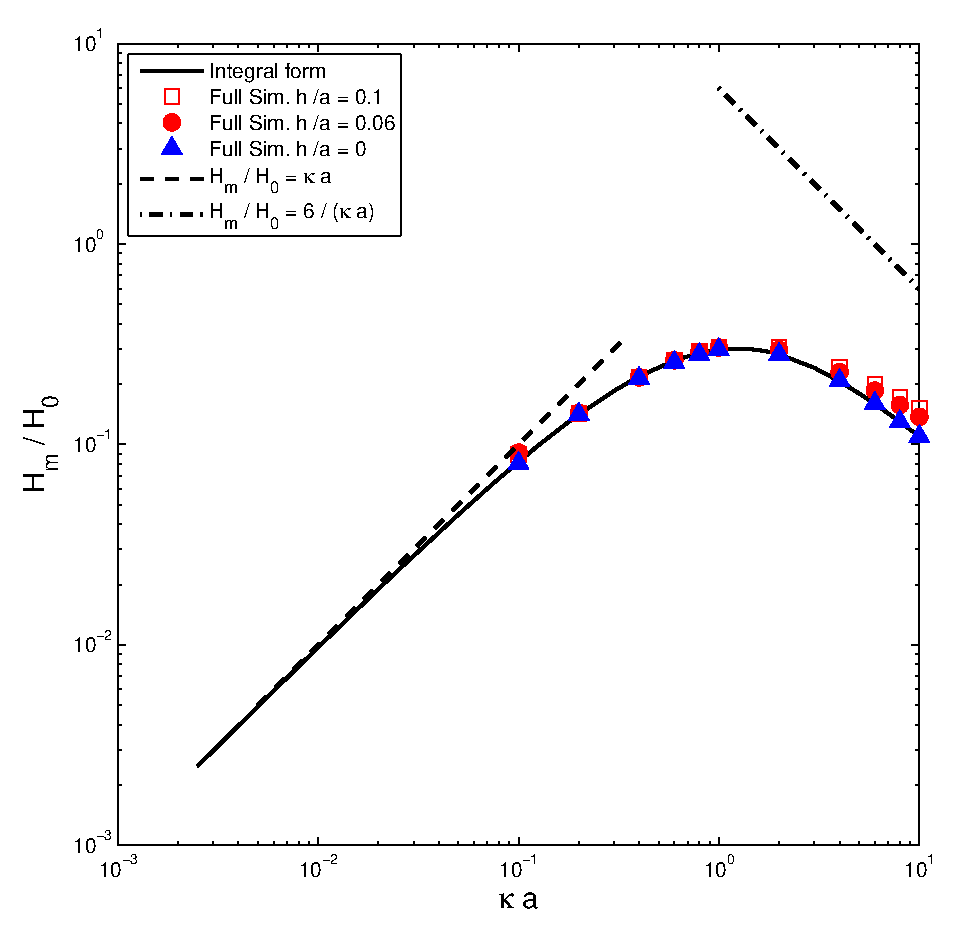
\includegraphics[width=0.46\textwidth]{finite_thickness/HmOverH0LogLog3}
\end{center}
\caption{The electroosmotic coefficient $H_{m}$, scaled by $H_0$ (Equation \ref{H0_defn}), for a membrane of thickness $h=0$, as a function of $a\kappa$. Solid line, analytic result (Equation \ref{reciprocal_integral}); dashed line, asymptote (Equation \ref{H_m_akappa_small}) for $a\kappa\ll 1$;
triangles: full PNP numerical computation ($h=0$). The dot-dashed line shows $H_{m}/H_0=6/(a\kappa)$ with the expected slope for large $a\kappa$. Squares and circles show electroosmotic coefficients $H/H_0$ for non-zero membrane thickness $h>0$, computed by numerical integration of the full PNP equations: solid circles  $h/a=0.06$; open squares $h/a=0.1$.}
\label{Fig:H_m_log_log}
\end{figure}

The membrane has zero thickness, so that there is always a region near
the edge of the pore where the Debye length $\kappa^{-1}$ cannot be
considered small compared with $h$:
Smoluchowski's analysis for thin charge
clouds, which would predict $H=6H_0/(a\kappa)$ if $\zeta_m$ took the
uniform value $(\epsilon\kappa)^{-1}\sigma_m$,
therefore cannot automatically be invoked when $a\kappa\gg 1$.
However, if we set up a local coordinate $s$ indicating distance from
the edge of the pore, both the electric potential $\chi$ (Equation \ref{chi_m})
and the fluid velocity $\mathbf{G}^m$ (Equation \ref{u_membrane})
vary as $s^{1/2}$ when $s\ll a$ (i.e. near the pore edge).
The charge cloud density $\rho_0$ decays over a lengthscale $\kappa^{-1}$,
and only counter-ions of membrane surface charge within a distance $\kappa^{-1}$
from the edge contribute to $\rho_0$ within the hole. The contribution
of the edge to the integral (Equation \ref{reciprocal_integral})
is therefore $O((a\kappa)^{-1})$,
as was similarly found for the electrophoretic velocity of a charged disk \cite{Sherwood1995}.
We therefore expect
$H_m\sim H_0/(a\kappa)$ when $a\kappa\gg 1$. The data in
Figure \ref{Fig:H_m_log_log} do not extend to sufficiently high
values of $a\kappa$ to allow us to estimate the asymptote with
any accuracy, and for the figure we simply indicate the line
$H_m/H_0=6/(a\kappa)$ suggested by the Smoluchowski analysis.
A similar reduction in the broadside electrophoretic velocity of a disk
below the value predicted by Smoluchowski was
noted by Sherwood \& Stone.\cite{Sherwood1995}
Individual points in Figure \ref{Fig:H_m_log_log}
indicate results obtained from full numerical solutions of
the Poisson-Nernst-Planck equations in a symmetric electrolyte
at low applied potential and low surface charge. 
In the computations, the length of
the reservoirs in the $z$ direction was equal to their
radius $b$, with $b=\max(10a,10\kappa^{-1})$.
Other details of the computations are reported in section \ref{sec:finite_numerical}.

\subsection{Composite electroosmotic coefficient $H_{\rm comp}$}
\label{subsec:finite_composite2}
When $h>0$ it is natural to suppose that the electric field
outside
the membrane pumps fluid towards the cylindrical pore at a rate
\begin{equation}
Q_{me}\approx H_m(\phi_1-\phi_2),
\label{q_me}
\end{equation}
and the electric field within the cylindrical pore
pumps fluid through the pore at a rate
\begin{equation}
Q_{ce}\approx H_c\phi_2.
\label{q_ce}
\end{equation}
However, in general, $Q_{me}$ (Equation \ref{q_me}) and
$Q_{ce}$ (Equation \ref{q_ce}) differ, and a pressure $\pm p_2/2$ builds
up at $z=\pm h/2$ (i.e. at the entrance and exit to the cylindrical pore)
in order to ensure that the volumetric flow rate is
continuous. We now determine this pressure $p_2$.

Consider a membrane of zero thickness ($h=0$), with pressure $p=p_1/2$
(above the reference ambient pressure)
at infinity on the side $z>0$, and with $p=-p_1/2$ at infinity on
the other side. The pressure within the hole in the membrane is
\begin{equation}
p=0,\quad z=0,\ r<a,\ h=0.
\end{equation}
The fluid velocity generated by the pressure difference $p_1$
across the membrane is
$\mathbf{u}=p_1\mathbf{G}^m$ (Equation \ref{u_membrane}),
and the corresponding volumetric flow rate is \cite{Happel&Brenner} %% revision - a cite added for flow rate 
\begin{equation}
Q_{mh}=G_mp_1,\quad G_m=-\frac{a^3}{3\mu}.
\end{equation}

If $h>0$ we approximate the pressure field in the fluid in much the same way as
we approximated the electrical potential within the fluid:
we patch a linearly varying pressure $p(z)$ within the
cylindrical pore to the pressure field outside a membrane of zero thickness,
and we take the pressure over the two ends $z=\pm h/2$ of the cylindrical
pore to be $\pm p_2/2$.
Thus the pressure within the pore is approximated as
\begin{equation}
p=\frac{p_2}{h}z,\quad r<a,\ |z|<h/2,
\end{equation}
the fluid velocity within the pore is
\begin{equation}
\mathbf{u}=p_2\mathbf{G}^c,
\label{u_c}
\end{equation}
and the volumetric flow rate within the pore is
\begin{equation}
Q_{ch}=G_cp_2,\quad G_c=-\frac{\pi a^4}{8h\mu}.
\label{G_c}
\end{equation}
Outside the cylindrical pore, the fluid velocity is assumed now to be
\begin{equation}
\mathbf{u}=(p_1-p_2)\mathbf{G}^m(r,z-h/2),\quad z>h/2,
\label{u_m}
\end{equation}
with $u_r(r,z)=-u_r(r,-z)$ and $u_z(r,z)=u_z(r,-z)$. 
The volumetric flow rate outside the membrane is now
\begin{equation}
Q_{mh}=G_m(p_1-p_2),\quad G_m=-\frac{a^3}{3\mu}.
\label{G_m}
\end{equation}
We have
ensured that the pressure (but not the fluid
velocity nor the volumetric flow rate) is continuous across the ends
$z=\pm h/2$ of
the cylindrical pore.

When an electric field generates an electroosmotic velocity, the
volumetric flow rates within the cylindrical pore and outside the
membrane are identical if $p_2$ is such that $Q_{mh}+Q_{me}=Q_{ch}+Q_{ce}$,
i.e. if
\begin{equation}
G_m(p_1-p_2)+H_m(\phi_1-\phi_2)=G_cp_2+H_c\phi_2.
\end{equation}
But the pressure at infinity is zero in the electroosmotic problem, so
$p_1=0$, and $\phi_2$ is given by Equation \ref{phi_2}.
Hence
\begin{equation}
p_2=
\frac{H_mR_m-H_cR_c}{(G_m+G_c)(R_m+R_c)}\phi_1,
\end{equation}
and the total electro-osmotic flow is
\begin{equation}
Q_E=Q_{me}+Q_{mh}=
\frac{(G_mR_cH_c+G_cH_mR_m)}{(R_m+R_c)(G_m+G_c)}\phi_1=H_\text{comp}\phi_1.
\label{flow_rate_lumped_parameter}
\end{equation}
An alternative derivation of this approximate composite
$H_\text{comp}$ (Equation \ref{flow_rate_lumped_parameter}) is given in the next
section.

Inserting into Equation \ref{flow_rate_lumped_parameter}
the various estimates for $G_m$ (Equation \ref{G_m}), $G_c$ (Equation \ref{G_c}),
$R_m$ (Equation \ref{Im_h0}) and $R_c$ (Equation \ref{I_c}),
we obtain
\begin{equation}
H_\text{comp}=
\frac{\left(H_m+\frac{16 h^2}{3\pi^2a^2}H_c\right)}
{\left(1+\frac{2h}{\pi a}\right)
\left(1+\frac{8h}{3\pi a}\right)}.
\label{H_comp}
\end{equation}
For small $h/a$ the approximate composite $H_\text{comp}$
is
larger than $H_m$ if
\begin{equation}
\frac{H_c}{H_m}>\frac{7\pi a}{8h}.
\label{H_c_for_H_comp_increasing}
\end{equation}
%%%%%% revision -- referee 2 %%%%
Experimental arrangements sometimes involve measurements at fixed current,
and a coefficient $K_\text{comp}$ that gives the electroosmotic
flux per unit current is therefore useful.
This quantity may be obtained readily from Equation \ref{I_c}, Equation \ref{phi_2} and Equation \ref{flow_rate_lumped_parameter}:
\begin{equation} 
K_\text{comp} = - \frac{Q_E}{I_c} = 
\frac{(G_mK_c+G_cK_m)}{(G_m+G_c)} = 
\frac{\left(K_m+\frac{8h}{3\pi a}K_c\right)}
{\left(1+\frac{8h}{3\pi a}\right)},
\label{K_comp}
\end{equation}
which changes from $K_m$ when $h=0$ to $K_c$ when $h\gg a$.

\subsection{Composite electroosmotic coefficient $H_{\rm comp}$
derived via the reciprocal theorem}
\label{subsec:finite_composite1}
We now show that approximations to the electric potential $\chi$ and
pressure-driven velocity $\mathbf{G}$ within a pore of non-zero length $h>0$,
when inserted into the integral expression (Equation \ref{reciprocal_integral})
for the electroosmotic
volume flux, lead to an approximate electroosmotic coefficient
identical to $H_\text{comp}$ (Equation \ref{H_comp}) obtained in the previous section.

We have already shown that we may approximate the electric potential
by a composite potential (Equation \ref{approx_chi_c}), (Equation \ref{approx_chi_m}), of the form
\begin{subeqnarray}
\chi&=&\left(\frac{z}{h}\right)\frac{R_c\phi_1}{R_m+R_c},\hskip 80pt |z|<h/2,
\\
&=&\frac{R_c\phi_1}{2(R_m+R_c)}+\frac{R_m\phi_1}{R_m+R_c}
\tilde\chi_m(r,z-h/2),
\hskip 10pt z>h/2,
\\
&=&\chi(r,-z),\hskip 90pt z<0.
\label{chi_approx_composite}
\end{subeqnarray}
%%% JOHN: I modified this sentence because here you are talking about 
% the flow generated under the sole influence of pressure. I worried that 
% this point would be lost on the reader OK, noted.
%We now create a similar approximation for the fluid velocity.
We now create a similar approximation for the fluid velocity for flow 
through a membrane of thickness $h$ subjected only to a pressure drop $p_1$ 
but no applied potential drop.
%%%%%%%%%%%
We suppose that in $z>h/2$ the fluid velocity is given by (Equation \ref{u_m}),
corresponding to flow outside a membrane of zero thickness, and that
within the cylindrical pore the fluid velocity is given by
(Equation \ref{u_c}). Continuity of the volumetric flow rates (Equation \ref{G_c}), (Equation \ref{G_m}) at the entrance to
the cylindrical pore requires that the pressure
$\pm p_2/2$ at the two ends of the pore satisfies
\begin{equation}
G_cp_2=G_m(p_1-p_2),
\end{equation}
so that
\begin{equation}
p_2=\frac{G_mp_1}{G_c+G_m}.
\end{equation}
Hence our approximation to the fluid velocity
is $\mathbf{u}=\mathbf{G}p_1$, with
\begin{subeqnarray}
\mathbf{G}&=&
\frac{G_m}{G_c+G_m}\mathbf{G}^c(r,z),\hskip 65pt |z|<h/2,
\\
&=&\frac{G_c}{G_c+G_m}\mathbf{G}^m(r,z-h/2),\hskip 30pt z>h/2.
\label{G_approx_composite}
\end{subeqnarray}
The (small) errors involved in this approximation are discussed by
Dagan et al.\cite{dagan1982}.

We now use the approximations (Equation \ref{chi_approx_composite}) and
(Equation \ref{G_approx_composite}) in the integral (Equation \ref{reciprocal_integral}) in order to
compute the electroosmotic volumetric flow rate. But the integration
splits naturally into an integral over the cylindrical pore and an
integral over the regions outside the membrane. The integral over the
cylindrical pore is exactly the integral required to determine
the electroosmotic flow rate $H_c$ (Equation \ref{Hc_defn}) in a cylinder, and the
integral outside the membrane is exactly that required to determine
$H_m$ (Equation \ref{Hm_defn}). Hence the integral yields the composite
electroosmotic flow rate
\begin{equation}
H_\text{comp}= \frac{G_cR_mH_m}{(G_c+G_m)(R_m+R_c)}
+\frac{G_mR_cH_c}{(G_c+G_m)(R_m+R_c)}
=\frac{G_cR_mH_m+G_mR_cH_c}{(G_c+G_m)(R_m+R_c)},
\end{equation}
identical to (Equation \ref{flow_rate_lumped_parameter}), obtained in section \ref{subsec:finite_composite2} by
elementary methods.

\subsection{Predictions of the composite electroosmotic coefficient}
\begin{figure}[H]
\begin{center}
\includegraphics[width=\textwidth]{finite_thickness/finite_pore_pic3.eps}
\caption{\label{Fig:H_comp}
The electroosmotic coefficient $H$ scaled by $H_0$ (Equation \ref{H0_defn}) for
$\sigma_m=\sigma_c$, as a function of $h/a$, for
(a) $a\kappa=10$, (b) $a\kappa=2$, (c) $a\kappa=1$,
 (d) $a\kappa=0.1$.
Solid lines, $H_{comp}$ (Equation \ref{H_comp});
solid circles: full PNP numerical computation.}
\end{center}
\end{figure}

\begin{figure}[H]
\begin{center}
\includegraphics[width=\textwidth]{finite_thickness/finite_pore_pic7.eps}
\caption{The results of Figure \ref{Fig:H_comp}, presented in terms of the electroosmotic coefficient $K=HR_{tot}$ scaled by $K_0$ (Equation \ref{K0_defn}) for $\sigma_m=\sigma_c$, as a function of $h/a$, for (a) $a\kappa=10$, (b) $a\kappa=2$, (c) $a\kappa=1$, (d) $a\kappa=0.1$. Solid lines, $K_{comp}$ (Equation \ref{K_comp}); solid circles: full PNP numerical computation.}
\label{Fig:K_comp}
\end{center}
\end{figure}

Figure \ref{Fig:H_comp} shows $H_\text{comp}$ (Equation \ref{H_comp}) as a function of $h/a$, for four
different values of $a\kappa$, with $\sigma_m=\sigma_c$. Also shown are the results of full numerical
computations based on the
Poisson-Nernst-Planck equations \cite{mao2014}
and described in section \ref{sec:finite_numerical}. 
The coefficient $H_c$ (Equation \ref{Hc_defn})
is proportional to $h^{-1}$ and is very large when the
pore length $h$ is small, leading to a large electroosmotic coefficient
$H_\text{comp}$. The action of the electric field
acting on charge confined within the cylindrical pore
is much more efficient at creating fluid motion than is the
weaker electric field acting on charge outside the pore.
We see that for $a\kappa\ge 1$ the
approximate analysis captures the main features of the full numerical
results, and it is clear from (Equation \ref{H_comp}) that it also has the
correct limits as $h/a\rightarrow 0$ and
$h/a\rightarrow\infty$. However,
it is also evident from Figure \ref{Fig:H_comp}(d)
that the theory is unsatisfactory when
$a\kappa\ll 1$.

The results of Figure \ref{Fig:H_comp}
are presented in terms of the coefficient $K_\text{comp}$
(Equation \ref{K_comp}) in Figure \ref{Fig:K_comp}. Both $K_\text{comp}$
and the full numerical results now increase monotonically with $h$,
with a final end point $K_\text{comp}=K_c$ that is independent of
$h$ when $h\gg a$. Figure \ref{Fig:K_comp}, like Figure \ref{Fig:H_comp},
shows that the theory leading to $K_\text{comp}$ is
inadequate when $a\kappa\ll 1$.
We discuss this limit in section \ref{sec:finite_overspill}, where
we shall show that when $a\kappa\ll 1$ some of the charge cloud of ions
that neutralizes the surface charge on the cylindrical wall of the pore
spills out of the ends of the pore, where it is less effective at generating
electroosmotic flow. The scenario is shown schematically in 
Figure \ref{Fig:schematic_overspill}.

\section{Numerical simulation}
\label{sec:finite_numerical}
The time-independent PNP--Stokes equations governing the electrical potential
$\phi$, the ionic number density of the $i$th ionic species $n^i$
($i=1,\dots,N$), the fluid velocity $\mathbf{u}$ and fluid pressure $p$
are
\begin{eqnarray}
\epsilon \nabla^2 \phi + \sum_{i=1}^{N} z_i e n^i & = & 0,
\label{eq:poisson_finite}
\\
\nabla\cdot\left\lbrack n^i\mathbf{u} -\omega^i(kT \nabla
n^i + ez_in^i\nabla\phi) \right\rbrack&=&0 ,
\label{eq:NP}
\\ 
-\nabla p + \mu \nabla^2 \mathbf{u} -  \nabla \phi \sum_{i=1}^{N} z_ien^i & = & 0, \label{eq:stokes_finite}\\
\nabla \cdot \mathbf{u} & = & 0, \label{eq:continuity_finite}
\end{eqnarray}
where $z_i$ is the valence of the $i$th ionic species and $\omega^i$
its mobility. Here we restrict our attention to the case
$N=2$, with $z_1=-z_2=1$.

We used a finite volume numerical scheme to
solve the system of coupled equations (Equation \ref{eq:poisson_finite})-(Equation \ref{eq:continuity_finite}) 
in the axisymmetric geometry depicted in Figure \ref{Fig:schematic}.
Thus, we considered a cylindrical pore of radius $a$ and length $h$ connecting two large cylindrical reservoirs of radius $b$. The lengths of AB and EF in our simulation were also taken to be $b$, which was kept much larger than either $a$ or the Debye length 
$\kappa^{-1}$ so that the reservoirs were effectively infinite.

{\it Boundary conditions.} At A and F, the two ends of the reservoirs, ion concentrations were set equal to the concentration in the bulk electrolyte (i.e. $n^i = n^{i}_{\infty}$); a potential difference $\Delta V$ was applied across the system by setting $\phi$ to $\pm \Delta V/2$ respectively at A and F where the pressures were set equal to the bulk pressure, $p = p_\infty$. At AB and EF, the side walls of the cylindrical reservoir, the radial component of the electric field, ionic flux and velocity were all set to zero, as was the tangential shear stress, in order to minimize the effect of these boundaries.
The last condition was imposed as the cylindrical reservoirs merely represent a convenient 
computational domain; the walls of the real physical reservoir are far enough away from the pore to be essentially irrelevant.
At the membrane and pore surfaces BC, CD and DE, a no--flux condition was used for (Equation \ref{eq:NP}), and a no--slip condition was used for the flow. At solid-fluid interfaces (with unit normal $\hat{n}$)
the electric potential is continuous but the normal component of the electric field undergoes a jump, with
$[ \epsilon \mathbf{E}\cdot \hat{n} ] = \sigma_m$ at BC and DE, 
and $[ \epsilon \mathbf{E}\cdot \hat{n} ] = \sigma_c$ at CD.

An electrohydrodynamic solver was implemented to solve the system described above using the OpenFOAM CFD library \cite{OPENFOAM}, a C++ library designed for computational mechanics. A structured mesh was constructed by means of the polyMesh
meshing tool within OpenFOAM. The grid was refined near the membrane and pore surfaces to resolve the Debye layer. Grid independence was checked in all cases by refining the grid and verifying that the 
solution did not change within specified tolerances.

For the finite volume discretization of the governing equations, central differences were used for all diffusive terms in (Equation \ref{eq:NP}) and viscous terms in (Equation \ref{eq:stokes_finite}). A second--order upwind scheme was used for the convective terms in (Equation \ref{eq:NP}). The discretized linear system was solved using a pre-conditioned conjugate gradient solver if the matrix was symmetric or a pre-conditioned bi--conjugate gradient solver if the matrix was 
asymmetric \cite{ferziger&peric}. 

An iterative scheme was used to solve the PNP--Stokes equations. Initially, the flow velocity 
was set to zero. Equations  (Equation \ref{eq:poisson_finite}) and (Equation \ref{eq:NP}) were then solved sequentially in a loop with under-relaxation (to ensure stability of the nonlinear PNP system) until the absolute residual was smaller than a specified tolerance -- in our case, $10^{-6}$.
 The electric force density $- \nabla \phi\sum_i z_ien^i $ was then obtained from this solution and used 
 as an explicit external forcing in the solution of the incompressible Stokes flow problem,
 (Equation \ref{eq:stokes_finite}) and (Equation \ref{eq:continuity_finite}), solved by means of the SIMPLE algorithm.  The flow field so computed was then substituted into (Equation \ref{eq:NP}) and the PNP equations were solved again using the updated flow field. An outer loop was constructed to iterate over the PNP loop and Stokes flow module, until the solution changed negligibly between two outer iterations.

Our main object of interest is the volumetric flux, $Q$. This was obtained by numerically integrating the axial velocity over the plane $z = 0$.
At the low voltages employed, the linear relation found between 
$Q$ and $\Delta V$ leads to the electroosmotic coefficient $H = Q/ \Delta V$,
shown as discrete points in Figures \ref{Fig:H_m_log_log}, \ref{Fig:H_comp},
\ref{Fig:K_comp}
and \ref{Fig:H_comp_akappa_small}.
The amount of charge within the pore was determined by numerical integration,
and used to obtain the quantities $h_\text{lost}$ and $h_\text{gained}$
reported below in Table 1.


\section{Charge overspill from the ends of the pore, $a\kappa\ll 1$}\label{sec:finite_overspill}
\subsection{Overspill of charge from the end of a semi-infinite pore}
\begin{figure}
\begin{center}
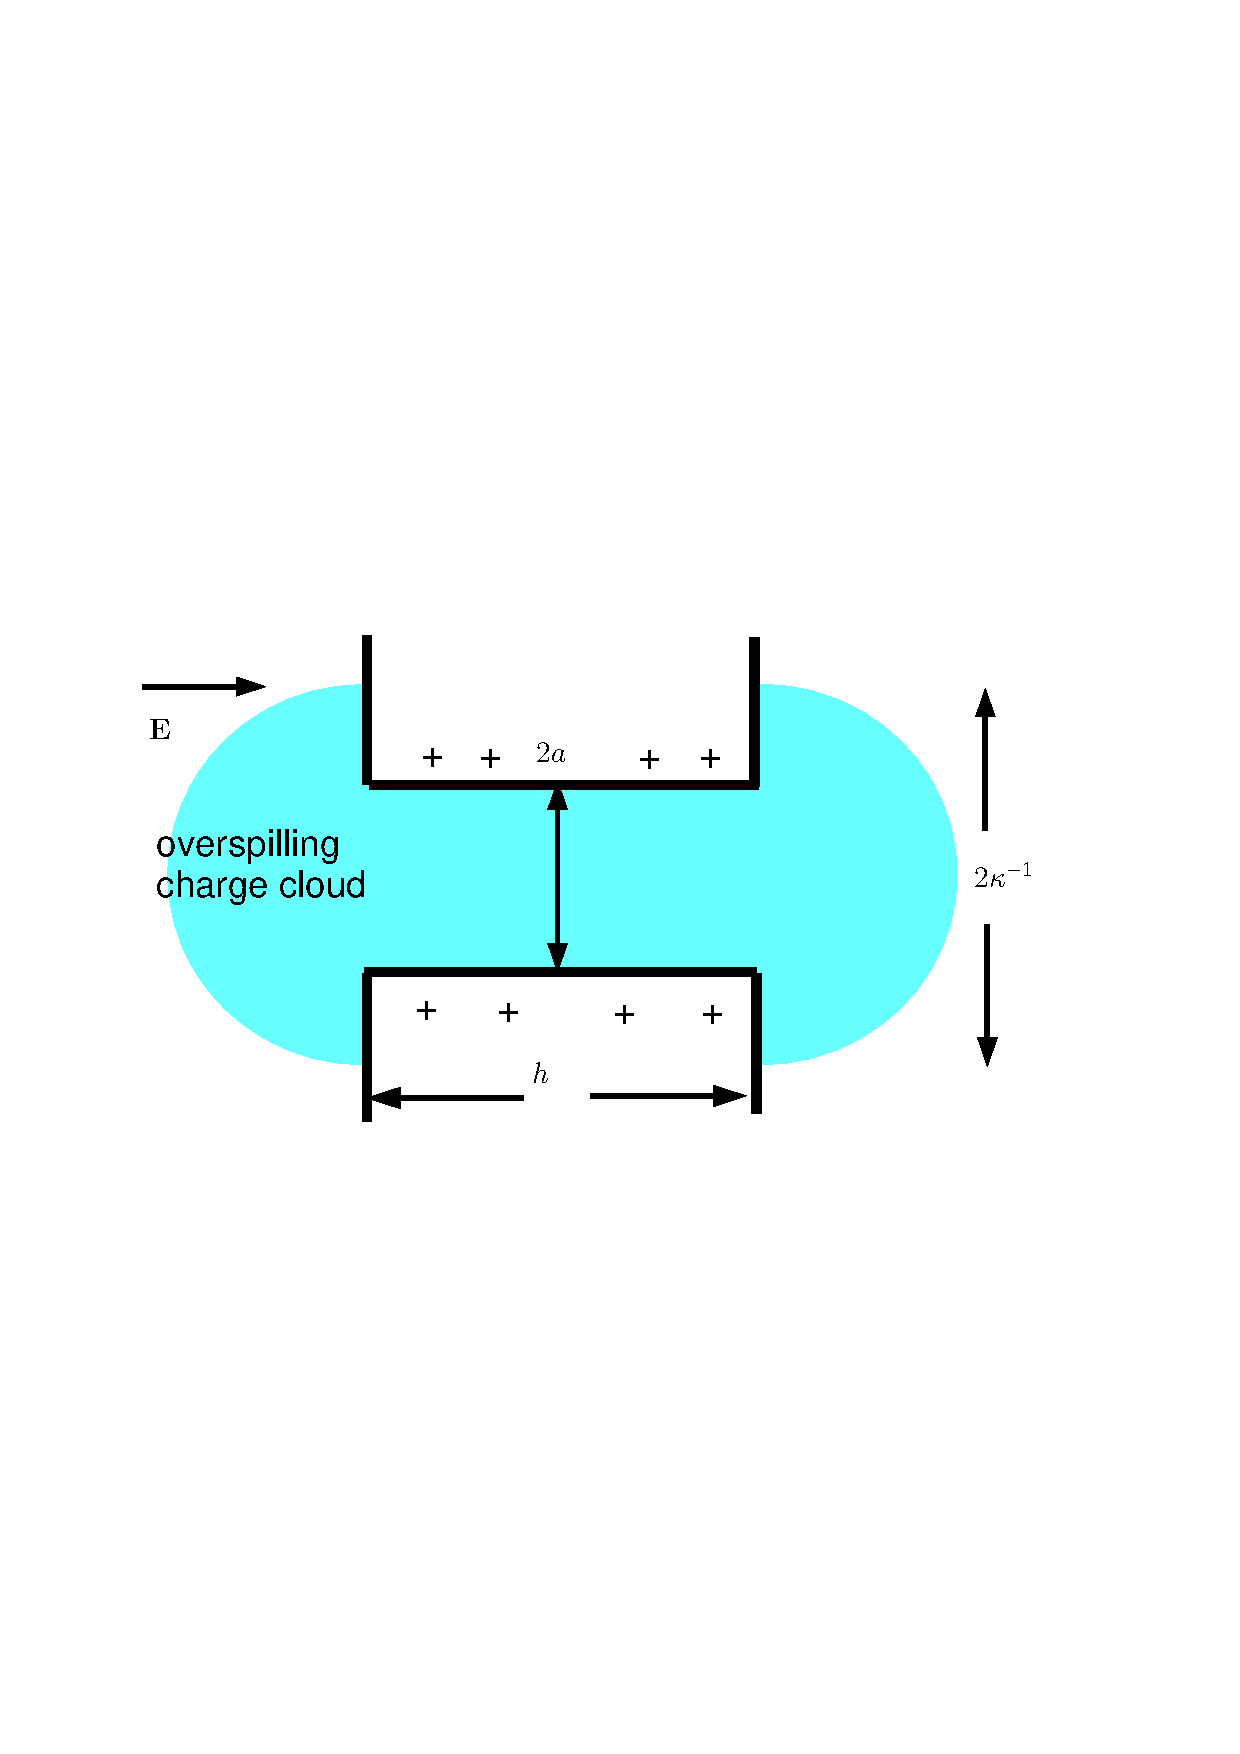
\includegraphics[width=0.6\textwidth]{finite_thickness/finite_pore_pic5}
\end{center}
\caption{When the Debye length $\kappa^{-1}$ is large compared with the pore radius $a$, the cloud of counter ions associated with the charged cylindrical wall of the pore spills out of the ends of the pore.}
\label{Fig:schematic_overspill}
\end{figure}

We consider a cylindrical pore of radius $a$, with surface charge density
$\sigma_c$. When the Debye length $\kappa^{-1}\gg a$,  the
equilibrium potential $\phi_0$ (Equation \ref{phi0_cylinder}) in an infinitely long cylinder can be expanded as
\begin{equation}
\phi_0=\phi_a
\left(1+\frac{(\kappa   r)^2}{4}+\cdots\right),
\end{equation}
where
\begin{equation}
\phi_a=\frac{\sigma_c}{\epsilon\kappa I_1(\kappa a)}
\approx\frac{2\sigma_c}{\epsilon\kappa(\kappa a)}.
\label{phi1_defn}
\end{equation}
Thus the equilibrium potential $\phi_0$ and charge density
$\rho_0=-\epsilon\kappa^2\phi_0$
within the charge cloud vary little over the
cross-section of the pore. On the other hand, if the cylinder is not
infinitely long and uniform, $\phi_0$ and $\rho_0$ vary
in the axial ($z$) direction with a length scale $\kappa^{-1}$.
We can therefore consider the equilibrium potential $\phi_0$ 
within the cylindrical pore to be a function only of
$z$ \cite{singer2009}.



We first consider a semi-infinite, charged cylindrical pore going from $z=0$
to $z=\infty$. The equilibrium potential $\phi_0$
satisfies a one-dimensional Poisson-Boltzmann
equation,
\begin{equation}
\frac{\text{d}^2\phi_0}{\text{d}z^2}=-\kappa^2\phi_0.
\label{1D_PB_eqn}
\end{equation}
The solution that tends to the uniform potential $\phi_a$ within the
pore as $z\rightarrow\infty$ far from the pore end at $z=0$, is
\begin{equation}
\phi_0=\phi_a-A\exp(-\kappa z),
\label{phi_semi_infinite}
\end{equation}
for some unknown constant $A$. 
The charge density within the charge cloud
inside the pore is $-\epsilon\kappa^2\phi_0$, and when the cylindrical
pore is infinite (and hence uniform) the charge per unit length in the
charge cloud is $-\pi a^2\epsilon\kappa^2\phi_a=-2\pi\sigma_ca$, equal
and opposite to the charge per unit length on the pore walls. When the
pore is semi-infinite, with a non-uniform charge
cloud (Equation \ref{phi_semi_infinite}), the
total charge that is lost from within the pore is
\begin{equation}
q_\text{lost}=-\pi a^2\epsilon\kappa^2\int_0^\infty (\phi_a-\phi_0)\,\text{d}z
=-\pi a^2\kappa\epsilon A.
\label{q_lost_one_end}
\end{equation}
At the end of the pore ($z=0$) the potential
is $\phi=\phi_a-A$.  

In $z<0$ the charge
cloud is no longer confined by the walls of the cylindrical pore
and spreads out radially: it is no longer possible to assume that
$\phi_0$ is a function of $z$ alone. 
We therefore need to solve the linearized Poisson-Boltzmann equation in the half-space $z<0$,
with $\phi_0=\phi_a-A$ over the region $z=0$, $r<a$ and
$\partial\phi_0/\partial z=0$ on $z=0$, $r>a$. At large distances from the
end of the pore, the potential decays as $\exp(-\kappa R)/R$,
where $R=(z^2+r^2)^{1/2}$ is a spherical polar coordinate,
but in the important region $R=O(a)$ the potential can be approximated by
the electrostatic potential corresponding to a solution of the Laplace
equation (i.e. $\kappa=0$). Hence, from (Equation \ref{chi_m}),
\begin{equation}
\phi_0=(\phi_a-A)\frac{2}{\pi}\tan^{-1}\left(\frac{1}{\sinh\xi}\right).
\label{laplace_disk}
\end{equation}
To relate the potential (Equation \ref{laplace_disk}) to the amount of charge
in the overspilling charge cloud (in $z<0$), we note that
the charge on one side of a charged disk at uniform potential
$(\phi_a-A)$ in unbounded space is 
$q=4a\epsilon(\phi_a-A)$.
Alternatively, one can argue that
far from the plane $z=0$, the spherical distance $R\approx a\cosh\xi$,
so that the potential (Equation \ref{laplace_disk}) is approximately
\begin{equation}
\phi_0\approx (\phi_a-A)\frac{2a}{\pi R}.
\end{equation}
In a spherically symmetric geometry this field corresponds to the far
field around a point charge of magnitude $8a\epsilon(\phi_a-A)$,
and the total surface charge on one side of the disk is 
$q=4a\epsilon(\phi_a-A)$, in agreement with the charge obtained by considering
the capacitance of the disk. The charge in the overspill charge cloud in $z<0$
is equal and opposite to $q$, and is therefore
\begin{equation}
q_\text{overspill}=-4a\epsilon\phi_0(z=0)=-4a\epsilon(\phi_a-A).
\label{capacitance_disk}
\end{equation}
But the total charge (Equation \ref{capacitance_disk}) in the overspill
outside the end of the pore must be
equal to the charge (Equation \ref{q_lost_one_end})
that has been lost from within the pore.
Hence
\begin{equation}
4a\epsilon(\phi_a-A)=\pi a^2\kappa\epsilon A,
\end{equation}
so that
\begin{equation}
A=\frac{\phi_a}{1+\pi a\kappa/4},
\end{equation}
and the potential at the end of the pore is
\begin{equation}
\phi_a-A=\frac{\phi_a}{1+4/(\pi a\kappa)}.
\end{equation}
The charge that has been lost from the end of the
pore is equivalent to the charge usually found in a pore of length
\begin{equation}
h_\text{lost}=-\frac{q_\text{overspill}}{2\pi a\sigma_c}
=\frac{4}{4\kappa+\pi a\kappa^2}.
\label{h_lost_one_end}
\end{equation}
The loss of charge implies that the combined charge cloud and wall
surface charge
over a cross section of constant $z$ are no longer electrically neutral,
as pointed out by Baldessari and Santiago \cite{baldessari2008a, baldessari2009a}.

\subsection{Overspill from the two ends of a finite pore}
We can now perform the same analysis for a pore that
occupies the region $-h/2<z<h/2$. The equilibrium
potential within the pore has the form
\begin{equation}
\phi_0=C-B\cosh(\kappa z),
\label{phi0_inside_two_ends}
\end{equation}
where we have chosen the solution that is symmetric about the centre of
the pore at $z=0$. The charge that has been lost from within the
pore is
\begin{equation}
q_\text{lost}=-\epsilon\kappa^2\pi a^2
\left(\int_{-h/2}^{h/2}(\phi_0-\phi_a)\,\text{d}z\right)
=\epsilon\pi a^2\kappa^2\left\lbrack
\frac{2B}{\kappa}\sinh\left(\frac{\kappa h}{2}\right)+(\phi_a-C)h\right\rbrack.
\label{q_lost_inside_two_ends}
\end{equation}
The total flux of electric field through the two ends of the pore
is
\begin{equation}
2\pi a^2\left.\frac{\partial\phi_0}{\partial z}\right|_{z=h/2}
=-2\pi a^2\kappa B\sinh\left(\frac{\kappa h}{2}\right).
\label{flux_though_two_ends}
\end{equation}
Comparing (Equation \ref{q_lost_inside_two_ends}) and
(Equation \ref{flux_though_two_ends}) we conclude that $C=\phi_a$. The potential
over the ends of the pore is
\begin{equation}
\phi_0(h/2)=\phi_0(-h/2)=\phi_a-B\cosh(\kappa h/2).
\end{equation}
The total charge in the two overspill charge clouds is therefore,
by (Equation \ref{capacitance_disk}),
\begin{equation}
q_\text{overspill}=-8a\epsilon\left\lbrack\phi_a
-B\cosh\left(\frac{\kappa h}{2}\right)\right\rbrack,
\label{q_overspill_two_ends}
\end{equation}
and this must be equal to the charge (Equation \ref{q_lost_inside_two_ends})
lost from within the pore. Hence
\begin{equation}
B=\frac{4\phi_a}{4\cosh(\kappa h/2)+\pi a\kappa\sinh(\kappa h/2)}
\label{B}
\end{equation}
and
\begin{equation}
\phi_a-B\cosh\left(\frac{\kappa h}{2}\right)=
\frac{\phi_a\pi a\kappa\sinh(\kappa h/2)}{4\cosh(\kappa h/2)+\pi
  a\kappa\sinh(\kappa h/2)}.
\label{phi_a_minus_B_cosh}
\end{equation}
The total charge that has been lost (from the two ends) is equivalent to a
total lost length
\begin{eqnarray}
h_\text{lost}=-\frac{q_\text{overspill}}{2\pi a\sigma_c}&=&
\frac{8\sinh(\kappa h/2)}
{4\kappa\cosh(\kappa h/2)+\pi a\kappa^2\sinh(\kappa h/2)}
\label{h_lost_two_ends}
\\
&\sim&\frac{8}{4\kappa+\pi a\kappa^2},\hskip 30pt \kappa h\gg 1,
\label{h_lost_two_ends_h_large}
\\
&\sim&\frac{4h}{4+\pi ah\kappa^2/2}
,\hskip 30pt \kappa h\ll 1.
\label{h_lost_two_ends_h_small}
\end{eqnarray}
We see from eqs (Equation \ref{h_lost_one_end}) and (Equation \ref{h_lost_two_ends_h_large}) 
that when $\kappa h\gg 1$ the lost charge is twice that lost
from a single end of a pore. We also note that $h-h_\text{lost}>0$, and that
when the pore is short ($\kappa h\ll 1$) the amount of charge
remaining within the cloud within the pore is proportional to
\begin{equation}
h-h_\text{lost}
\sim\frac{\pi a \kappa^2h^2}{8+\pi ah\kappa^2}
,\hskip 30pt \kappa h\ll 1.
\label{h_min_h_lost_h_small}
\end{equation}

\subsection{Overspill from the membrane surface into the pore}
\label{subsec:finite_overspill4-3}
If the cylindrical
pore itself is uncharged, but the membrane surfaces are charged, ions
from the charge cloud adjacent to the membrane surface
are able to move into the ends of the pore.

If the membrane has zero thickness,
the charge density $\rho_0$ in the equilibrium charge cloud is
given by (Equation \ref{eq:rho0_finite}), and
both $\rho_0$ and the potential $\phi_0=-\rho_0/(\epsilon\kappa^2)$
vary over the area of the pore. Nevertheless, we may work out the mean potential
over the circular pore,
\begin{equation}
\overline{\phi}_0=-\frac{1}{\epsilon\kappa^2\pi a^2}
\int_0^a 2\pi r\rho_0\,\text{d}r
=\frac{2\sigma_m}{\epsilon a}
\left\lbrack\frac{a}{2\kappa}-
 \int_0^\infty
\frac{aJ_1(as)J_1(as)}{s(\kappa^2+s^2)^{1/2}}\,\text{d}s
 \right\rbrack,
\end{equation}
where, when $a\kappa\ll 1$,
\begin{equation}
\int_0^\infty
\frac{aJ_1(as)J_1(as)}{s(\kappa^2+s^2)^{1/2}}\,\text{d}s
\approx a^2\int_0^\infty
\frac{J_1(t)J_1(t)}{t^2}\,\text{d}t
=\frac{4a^2}{3\pi}.
\end{equation}
Thus when the membrane has zero thickness (and there is no
cylindrical pore into which ions can escape)
the absence of surface charge over
the area of the pore
changes the average potential over the opening from 
the value
$\phi_0=\sigma_m/(\epsilon\kappa)$ due to a uniformly charged surface
to $\beta\sigma_m/(\epsilon\kappa)$, where
\begin{equation}
\beta\approx 1-\frac{8a\kappa}{3\pi},\hskip 20pt a\kappa \ll 1.
\label{beta_defn}
\end{equation}

We now consider the charge
that leaks into a pore of length $h>0$ from the charge clouds on either
side of the membrane.
We suppose that the potential on the planes
$z=\pm h/2$ is perturbed by an amount $D$, and becomes
\begin{equation}
\phi_0=\frac{\beta\sigma_m}{\epsilon\kappa}+D,\hskip 20pt z=\pm h/2.
\label{underspill_perturbed_potential}
\end{equation}
Within the pore, the potential obeys the 1-dimensional
Poisson-Boltzmann equation (Equation \ref{1D_PB_eqn}), with solution
\begin{equation}
\phi_0=\left(\frac{\beta\sigma_m}{\epsilon\kappa}+D\right)
\frac{\cosh(\kappa z)}{\cosh(\kappa h/2)},
\end{equation}
and the additional charge within the pore is
\begin{equation}
q_\text{in}-\epsilon\kappa^2\pi a^2\int_{-h/2}^{h/2}\phi_0\,\text{d}z
=-\pi a^2\left(\beta\sigma_m+D\epsilon\kappa\right)
\frac{2\sinh(\kappa h/2)}{\cosh(\kappa h/2)}.
\end{equation}
Outside the pore, the perturbed potential
(Equation \ref{underspill_perturbed_potential}) is associated with
a total additional charge (Equation \ref{capacitance_disk})
\begin{equation}
q_\text{out}=-8a\epsilon D
\label{q_out_underspill}
\end{equation}
on the two sides of the membrane.
But the total change in charge caused by this redistribution must be zero,
i.e. $q_\text{in}+q_\text{out}=0$. Hence
\begin{equation}
\pi a^2\left(\beta\sigma_m+D\epsilon\kappa\right)
\frac{2\sinh(\kappa h/2)}{\cosh(\kappa h/2)}
+8a\epsilon D=0,
\end{equation}
i.e.
\begin{equation}
D=-\frac{\pi a\beta\sigma_m\sinh(\kappa h/2)}
{[4\cosh(\kappa h/2)+\pi a\kappa\sinh(\kappa h/2)]\epsilon}.
\end{equation}
The total charge $q_\text{in}=-q_\text{out}$ (Equation \ref{q_out_underspill})
that leaks into the pore at the two ends
corresponds to the charge inside a uniformly charged
cylinder with surface charge density $\sigma_m$,  of length
\begin{eqnarray}
h_\text{gained}=-\frac{8a\epsilon D}{2\pi a\sigma_m}&=&\frac{4 a\beta\sinh(\kappa h/2)}
{4\cosh(\kappa h/2)+\pi a\kappa\sinh(\kappa h/2)}=\frac{a\kappa\beta}{2}h_\text{lost},
\label{h_gained}
\\
&\sim&\frac{a\kappa\beta h}{2},\hskip 20pt \kappa h\ll 1,
\label{h_gained_h_small}
\\
&\sim&\frac{a\beta}{2+\pi a\kappa},\hskip 20pt \kappa h\gg 1.
\end{eqnarray}
Thus $h_\text{gained}$ (Equation \ref{h_gained}) is smaller than
$h_\text{lost}$ (Equation \ref{h_lost_two_ends}) by a factor $a\kappa\beta/2$.
We can compare the
predictions (Equation \ref{h_lost_two_ends})
and (Equation \ref{h_gained}) against results
obtained from full numerical solution of the nonlinear Poisson-Boltzmann
equation with either $\sigma_m=0$ and
$ae\sigma_c/(\epsilon kT)=a\kappa e\zeta_c/(kT)=0.00273$,
or $\sigma_c=0$ and
$ae\sigma_m/(\epsilon kT)=0.00273$:
results for $a\kappa=0.1$ are given in Table 1. We see that there is
excellent agreement between the numerical computations and the analysis
presented above.

\begin{table}
\begin{center}
\begin{tabular}{cc @{\hspace{30pt}} cc @{\hspace{30pt}} cc}
$h/a$&$h\kappa$&\multicolumn{2}{c}{$h_\text{lost}/a$}
&\multicolumn{2}{c}{$h_\text{gained}/a$}
\\
&&theory (Equation \ref{h_lost_two_ends})&numerical&theory (Equation \ref{h_gained})&numerical
\\
10.0&1.0&8.9186&8.9249&0.4081&0.4119
\\
1.0&0.1&0.9953&0.9954&0.0455&0.0459
\\
0.1&0.01&0.1000&0.1000&0.0046&0.0046
\end{tabular}
\end{center}
\caption{The charge lost from the ends of a charged
pore when the membrane charge density $\sigma_m=0$, in terms of an
equivalent pore length $h_\text{lost}$ (Equation \ref{h_lost_two_ends}),
and the charge gained inside an uncharged pore ($\sigma_c=0$)
from the charge cloud adjacent to the charged membrane surfaces,
in terms of an equivalent pore length $h_\text{gained}$ (Equation \ref{h_gained}).
$a\kappa=0.1$.}
\end{table}


\subsection{Composite electroosmotic coefficient}
We first consider how the electroosmotic coefficients $H_c$ and $H_m$
are modified by the overspill of the charge cloud from inside the
cylindrical pore to outside the membrane.
If a uniform electric field of
strength $E=-\phi_1/h$ is applied between the ends of the pore,
the Navier Stokes equations for steady flow yield the axial velocity profile
\begin{equation}
u=\frac{a^2-r^2}{4\mu}\left(\rho_0E-\frac{{\rm d}p}{{\rm d}z}\right)
\end{equation}
so that the volumetric flow rate is
\begin{equation}
Q=\frac{a^4\pi}{8\mu}\left(\rho_0E-\frac{{\rm d}p}{{\rm d}z}\right).
\label{Q_in_uniform_pore}
\end{equation}
But $Q$ is independent of $z$ (by incompressibility), and the pressure $p$
difference between the two ends of the capillary is zero. Hence, integrating
(Equation \ref{Q_in_uniform_pore}) along the length $h$ of the cylindrical pore,
and noting that
the total amount of charge in the charge cloud remaining within
the pore is
$2\pi a\sigma_c(h-h_\text{lost})$, we find
\begin{equation}
Q=\frac{a^4\pi E}{8h\mu}\int_{-h/2}^{h/2}\rho_0\,\text{d}z
=\frac{\pi a^3\sigma_c(h-h_\text{lost})\phi_1}{4h^2\mu}
=H_c\phi_1,
\label{H_c_underspill}
\end{equation}
which may be compared to the result (Equation \ref{H_c_kappa_small})
which ignores overspill.
The charge cloud outside the pore is enhanced by the overspill, and becomes
(in $z>0$)
\begin{equation}
\rho_0
=-\sigma_m\kappa\exp(-\kappa z)
-\frac{2\epsilon\kappa^2}{\pi}\left\lbrack\phi_a-B\cosh(\kappa h/2)\right\rbrack
\tan^{-1}\left(\frac{1}{\sinh\xi}\right),
\end{equation}
with the final term $[\phi_a-B\cosh(\kappa h/2)]$,
corresponding to the overspill charge cloud
(Equation \ref{phi_a_minus_B_cosh}), being
approximately valid in a volume $O(a^3)$ around the pore, but invalid at large
distance $O(\kappa^{-1})$ from the pore, where the exponential decay
of the charge density
is not captured by the solution (Equation \ref{laplace_disk}) of the Laplace equation.
The volumetric flow rate through a pore of zero thickness created by
a potential difference $\phi_1$
is given by the integral (Equation \ref{reciprocal_integral})
and was shown by Mao et al. \cite{mao2014} to be:
\begin{eqnarray}
Q  &=&  \frac{2a^3\phi_1}{\pi\mu}
\int_0^{\frac{\pi}{2}} d\eta \int_0^\infty \rho_0
\frac{\cos^2\eta\sin\eta}{\cosh\xi} d\xi
\nonumber\\
&=&-\frac{a^3\kappa\sigma_m\phi_1}{3\mu}
-\frac{4\epsilon\kappa^2a^3\phi_1}{\pi^2\mu}(\phi_a-B)
\int_0^{\pi/2}\cos^2\eta\sin\eta\text{ d}\eta \int_0^\infty 
\tan^{-1}\left(\frac{1}{\sinh\xi}\right)\frac{\text{d}\xi}{\cosh\xi}
\nonumber\\
&=&-\frac{a^3\kappa\sigma_m}{3\mu}\phi_1
-\frac{4\epsilon a^3\kappa^2}{3\pi^2\mu}\phi_1(\phi_a-B)I_3,
\label{Q_integral_disk}
\end{eqnarray}
where
\begin{equation}
I_3=
\int_0^\infty 
\tan^{-1}\left(\frac{1}{\sinh\xi}\right)\frac{\text{d}\xi}{\cosh\xi}
=\int_0^\infty \tan^{-1}x\ \frac{\text{d}x}{1+x^2}
=\frac{\pi^2}{8}.
\end{equation}
Hence the electroosmotic flow rate $Q=H_m\phi_1$
due to the charge cloud outside the
membrane is modified, and $H_m$ becomes
\begin{equation}
H_m=\frac{a^3\kappa}{3\mu}\left\lbrack
\sigma_m+
\frac{\pi\sinh(\kappa h/2)\sigma_c}
{4\cosh(\kappa h/2)+\pi a\kappa\sinh(\kappa h/2)}
\right\rbrack.
\label{H_m_overspill}
\end{equation}

If $\sigma_m$ is comparable to $\sigma_c$, then we saw in Section \ref{subsec:finite_overspill4-3} that
the change in the charge within the pore due to the charge cloud outside
the membrane entering the pore is $O(a\kappa)$ smaller than the loss of
charge from the charge cloud within the pore to the regions
outside the membrane. However, this contribution can be included
with very little effort, and becomes important in the limit
$h\rightarrow 0$, when the gain (Equation \ref{h_gained_h_small})
in charge within the pore
from the outside surface charge density $\sigma_m$
is proportional to $h_\text{gained}\propto h$,
whereas the charge cloud (due to $\sigma_c$ within the pore)
remaining within the pore, is
proportional to $h-h_\text{lost}\propto h^2$, by
(Equation \ref{h_min_h_lost_h_small}).
The electroosmotic coefficient $H_c$
for the cylindrical pore (Equation \ref{H_c_underspill}) becomes
\begin{equation}
H_c=\frac{\pi a^3\sigma_c(h-h_\text{lost}+h_\text{gained}\sigma_m/\sigma_c)}
{4h^2\mu},
\label{H_c_overspill_underspill}
\end{equation}
and the electroosmotic coefficient $H_m$ for the charge cloud
outside the membrane (Equation \ref{H_m_overspill}) becomes
\begin{equation}
H_m=\frac{a^3\kappa}{3\mu}\left\lbrack
\sigma_m+
\frac{\pi\sinh(\kappa h/2)(\sigma_c-a\kappa\beta\sigma_m/2)}
{4\cosh(\kappa h/2)+\pi a\kappa\sinh(\kappa h/2)}
\right\rbrack.
\label{H_m_overspill_underspill}
\end{equation}

Now that $H_c$ (Equation \ref{H_c_overspill_underspill}) and 
$H_m$ (Equation \ref{H_m_overspill_underspill})
have been corrected for the effects of overspill
in the two directions, they can be inserted into the expression
(Equation \ref{H_comp})
for the composite electroosmotic coefficient $H_\text{comp}$.
Results are shown in Figure \ref{Fig:H_comp_akappa_small}(a), together
with full numerical solutions of the Poisson-Nernst-Planck equations.
We see that the agreement between theory and computation is much better
than  when overspill is ignored (Figure \ref{Fig:H_comp}(d)). 
Charge overspill or underspill causes the total charge of mobile ions
within the pore to differ
from what might be expected on the basis of net 
electroneutrality of the pore. 
Thus, the driving force is modified leading to deviations from the calculated 
result that ignores such effects. The ``lost length'' $h_\text{lost}$ in (Equation \ref{H_c_overspill_underspill})
restores this effect.
Figure \ref{Fig:H_comp_akappa_small}(b) shows the results of
Figure \ref{Fig:H_comp_akappa_small}(a) expressed in terms of
$K$, rather than $H$, and there is again good agreement between the
theoretical $K_\text{comp}$ and full numerical results.

\begin{figure}[h]
\begin{center}
\includegraphics[width=0.99\textwidth]{finite_thickness/finite_pore_pic8.eps}
\caption{\label{Fig:H_comp_akappa_small}
(a) The electroosmotic coefficient $H$ scaled by $H_0$ (Equation \ref{H0_defn}) for $\sigma_m=\sigma_c$, as a function of $h/a$, for $a\kappa=0.1$, including the effect of overspilling charge clouds. Solid lines $H_\text{comp}$ (Equation \ref{H_comp}), using $H_c$ given by (Equation \ref{H_c_overspill_underspill}) and $H_m$ given by (Equation \ref{H_m_overspill_underspill}); solid circles: full PNP numerical computation. c.f. Fig. \ref{Fig:H_comp}(d), in which overspill was neglected. (b) The same results, presented in terms of $K=R_\text{tot}H$ scaled by $K_0$ (Equation \ref{K0_defn}). Solid lines $K_\text{comp}$ (Equation \ref{K_comp}), using $K_c=R_cH_c$ and $K_m=R_mH_m$; solid circles: full computation. c.f. Fig. \ref{Fig:K_comp}(d).}
\end{center}
\end{figure}

Note that when $h\ll\kappa^{-1}$ the effective length of the
cylindrical pore $h-h_\text{lost}\approx \pi a\kappa^2h/2$,
by (Equation \ref{h_min_h_lost_h_small}). The approximation
(Equation \ref{H_c_overspill_underspill}) for $H_c$
is therefore dominated by the term $h_\text{gained}$,
and gives $H_c\sim \pi a^4\kappa\beta\sigma_m/(8h\mu)$, with
$H_c/H_m\sim 3\pi a\beta/(8h)$. We conclude from
(Equation \ref{H_c_for_H_comp_increasing}) that $H_\text{comp}$
is a decreasing function of $h$ near $h=0$, as seen in 
Figure \ref{Fig:H_comp_akappa_small}(a).


\section{Concluding remarks}
The analysis presented here shows that it is possible to use simple
analyses based on continuity of volumetric flow rate and electric
current to estimate electroosmotic
end effects in a charged cylindrical pore traversing
a membrane of thickness $h>0$. Note that we have made repeated
use of the assumption that surface charge densities, and corresponding
zeta potentials, are small. Not only have we worked
with the linearized Poisson-Boltzmann equation
(Equation \ref{eq:linear_poisson_boltzmann_eqn}), but we have used superposition to
combine various contributions to the charge clouds due to
overspill of the clouds from one region (inside/outside the pore) to the other.
At high potentials it would also be necessary to keep track of the
fluxes of individual ion species, rather than simply ensuring
that the total electrical current is continuous \cite{biscombe2012}.

%%%%%%  (revision- referee 1) %%%%%%
The assumption of small potentials also justifies our neglect of other 
nonlinear electrokinetic effects such as Induced Charge
Electroosmosis (ICEO) \cite{murtsovkin96, Squires2004} which can
produce vortices in the vicinity of sharp corners \cite{Thamida2002}
or near rapid constrictions in channels \cite{park2006eddies}
when the permittivity of the solid $\epsilon_s>0$.
However, numerical solutions confirm the expectation that the flow rate is only weakly affected by 
such vortices, particularly under conditions of small potentials \cite{Mao2013}.
%%%%%%%%%%%%%%%%%%

%%%%%%%% revision - referee 2 %%%%%%%
In recent experiments
\cite{ghosal2013Nanoletter,Keyser2006,Garaj2010,Schneider2010,Merchant2010} 
on nanopores, potential differences of $\Delta\phi \sim 0 - 200$~mV
were applied across the pore.
Here we have assumed that $\Delta\phi\ll\zeta$, where 
$\zeta$ itself is assumed small in comparison with the thermal voltage $kT/e \sim 25$ mV.
 Thus, our results can only be expected to describe the initial linear part of the current-voltage 
 and flow-voltage characteristics, even though numerical simulations seem to show \cite{Mao2013}
 that this linear regime extends to applied voltages $\sim 100\rm\ mV$.
%%%%%%%%%%%%%%%%%%%%%%%%%%%%

Finally, we point out that the
correction factor $\beta$ (Equation \ref{beta_defn})
reminds us that the hole in the charged membrane removes a circular
region of surface charge and reduces the equilibrium potential
at the entrance to the pore. The introduction of
$\beta<1$ improved the agreement between
theoretical and numerical results for $h_\text{gained}$ in Table 1.
However, the analysis is not rigorous, since the equilibrium
potential across the hole is not uniform. The $O(1-\beta)$
correction to the equilibrium potential corresponds to an $O(1-\beta)$
correction
to the charge density $\rho_0$.
If we use this in the integral expression
(Equation \ref{Q_integral_disk})
in order to determine a correction to the electroosmotic flow rate
through a membrane of zero thickness, the analysis suggests that the correction
to the leading order result (Equation \ref{H_m_akappa_small})
for $a\kappa\ll 1$ should be $O((a\kappa)^2)$,
whereas investigation of the difference (seen in Figure \ref{Fig:H_m_log_log})
between numerical results and the asymptote (Equation \ref{H_m_akappa_small})
indicates additional
corrections $O((a\kappa)^2\ln a\kappa)$.


%%%%%%%%%% Removed texts %%%%%%%%%%%%%%%%%
%The electroosmotic coefficient $H_{m}$, 
%scaled by $H_0$ (Equation \ref{H0_defn}), for a membrane of thickness $h=0$,
%as a function of $a\kappa$. \copy\grapha analytic result
%(Equation \ref{reciprocal_integral});
%\copy\graphf asymptote (Equation \ref{H_m_akappa_small}) for $a\kappa\ll 1$;
%blue trangles: full PNP numerical computation ($h=0$).
%The dotted line \copy\graphg\ shows $H_{m}/H_0=6/(a\kappa)$
%which has the slope expected for large $a\kappa$.
%Red symbols show electroosmotic coefficients $H/H_0$ computed numerically
%for non-zero membrane thickness: circles  $h/a=0.06$; open squares $h/a=0.1$.
%The electroosmotic coefficient $H_{m}$, 


%scaled by $H_0$ (Equation \ref{H0_defn}), for a membrane of thickness $h=0$,
%as a function of $a\kappa$. \copy\grapha analytic result
%(Equation \ref{reciprocal_integral});
%\copy\graphf asymptote (Equation \ref{H_m_akappa_small}) for $a\kappa\ll 1$;
%$\blacktriangleright$ full numerical computation ($h=0$).
%The dotted line \copy\graphg\ shows $H_{m}/H_0=6/(a\kappa)$
%which has the slope expected for large $a\kappa$.
%Also shown are electroosmotic coefficients $H/H_0$ computed numerically
%for non-zero membrane thickness: $\bullet$  $h/a=0.06$; $\square$ $h/a=0.1

\chapter{Electrically generated eddies at an eight-fold stagnation point
within a nanopore}\label{chpt:eddies}
%\DeclareMathAlphabet{\mathsfb}{OT1}{cmss}{bx}{n}
%\newcommand\sfbsS{\mathsfb{S}}
%\newcommand\sfbsI{\mathsfb{I}}
%\newcommand\sfbsT{\mathsfb{T}}
%\newcommand\sfbsE{\mathsfb{E}}
%\providecommand\bnabla{\boldsymbol{\nabla}}
%
%\newbox\grapha
%\newbox\graphf
%\newbox\graphg
%\newbox\graphh
%
%\setbox\grapha=\hbox{\hskip 2pt
%\vrule height3pt depth-2pt width 40pt
%\hskip 2pt}
%
%\setbox\graphf=\hbox{\hskip 2pt
%\vrule height3pt depth-2pt width 12pt
%\hskip 4pt
%\vrule height3pt depth-2pt width 12pt
%\hskip 4pt
%\vrule height3pt depth-2pt width 12pt
%\hskip 4pt
%\vrule height3pt depth-2pt width 12pt
%\hskip 4pt}
%
%\setbox\graphh=\hbox{\hskip 2pt
%\vrule height3pt depth-2pt width 9pt
%\hskip 4pt
%\vrule height3pt depth-2pt width 2pt
%\hskip 4pt
%\vrule height3pt depth-2pt width 9pt
%\hskip 4pt
%\vrule height3pt depth-2pt width 2pt
%\hskip 4pt
%\vrule height3pt depth-2pt width 9pt
%\hskip 4pt}
%
%\setbox\graphg=\hbox{\hskip 2pt
%\vrule height3pt depth-2pt width 2pt
%\hskip 4pt
%\vrule height3pt depth-2pt width 2pt
%\hskip 4pt
%\vrule height3pt depth-2pt width 2pt
%\hskip 4pt
%\vrule height3pt depth-2pt width 2pt
%\hskip 4pt
%\vrule height3pt depth-2pt width 2pt
%\hskip 4pt
%\vrule height3pt depth-2pt width 2pt
%\hskip 4pt
%\vrule height3pt depth-2pt width 2pt
%\hskip 4pt}

%\textwidth 16cm
%\hsize 16 cm
%\textwidth 17cm
%\hsize 17 cm
%\setlength{\hsize}{18 cm}
%\oddsidemargin 0pt
%\evensidemargin 0pt
%\parskip 15pt
%
%\baselineskip 20pt
%\textwidth 18cm
%\hsize 18 cm
%\setlength{\hsize}{18 cm}
%\oddsidemargin 0pt
%\evensidemargin 0pt
%\hsize 16 cm
%\textwidth 16cm
%\setlength{\hsize}{16 cm}
%\setlength{\textwidth}{16 cm}
%\setlength{\parindent}{0 pt}

%\begin{abstract}
%
%Electrically generated flows around a \textcolor{red}{thin} dielectric
%\textcolor{red}{plate} pierced by a cylindrical
%\textcolor{red}{hole}
%are computed numerically. \textcolor{red}{The geometry represents that
%of a single nanopore in a membrane}. When the membrane is uncharged, flow
%is due solely to induced charge electroosmosis, and eddies are generated by
%the high fields at the corners of the nanopore. These eddies meet at
%stagnation points. If the geometry is chosen correctly, the stagnation
%points merge to form a single stagnation point at which four streamlines
%cross at a point and eight eddies meet.
%\end{abstract}

\section{Introduction}

Streamline patterns reveal the topology of a flow field:
we sketch streamlines, eddies and stagnation points
in order to develop our understanding of flows
\cite{moffatt1964,jeffrey1980}.
Stagnation points away from solid walls usually occur at the intersection of
two streamlines, which divide the fluid into four separate regions.
Such stagnation points can be generated in many ways, e.g. by
a four-roll mill \cite{taylor1934} or by opposed fluid jets
in a cross-slot device \cite{scrivener1979,cachile2012}.
More complicated stagnation points are harder to generate.
Berry and Mackley \cite{berry1977} built  a six-roll mill and investigated
the flow field. When exact symmetry was achieved,
six eddies met at a central point, and the various ways in which
symmetry could be broken were described by Berry and Mackley
in terms of catastrophe theory. Here we report an electrically
generated flow
field in which four streamlines cross at a point and divide the flow into eight
regions.


\begin{figure}[h]
\begin{center}
\includegraphics[width=0.5\textwidth,clip=true]{eddies/eddy_fig1b.eps}
\end{center}
\caption{The (infinite)
dielectric plate of thickness $h$, pierced by a hole of radius $a$
and surrounded by
an electrolyte solution. 
The axisymmetric geometry represents a nanopore in a membrane.
An electrical current is driven through the hole by a potential difference
$\Delta\phi$ between the two sides, at infinity.}
\label{fig:hole}
\end{figure}


The axisymmetric flow geometry is shown in figure \ref{fig:hole}.
A cylindrical
hole of radius $a$ passes through an uncharged thin dielectric
plate of thickness $h$:
the hole represents a nanopore in a membrane, and we are interested in the
induced charge electroosmotic
flow generated by an electric potential difference applied 
between the two sides of the membrane \cite{Mao2013,mao2014,sherwood2014}.
We set up cylindrical polar coordinates, with $z$ axis along the axis of
symmetry and with the plane surfaces of the membrane at $r>a$,  $z=\pm h/2$.

In Section \ref{sec:imposed_electric} we consider the electric field passing through a circular hole in
a membrane of zero thickness. We then (Section \ref{sec:conformal_map})
show how the field is modified at
the edge of the hole when the membrane thickness $h$ is small but non-zero.
In Section \ref{sec:corner_charge}
we review the fluid jets that are created by the electrical
forces on 
%%%
the
%%%
fluid near the
corners of the membrane, and then in Section \ref{numerical_comp} we present 
numerical computations that show how the geometry of
eddies created by these jets depends on the geometry of the hole in
the membrane. As the ratio $h/a$ increases, three
stagnation points merge to form
a stagnation point at which four streamlines cross. The
stagnation points separate again
as $h/a$ increases further.

\section{The imposed electric field\label{sec:imposed_electric}}

The pore
and the two regions on either side of the membrane are occupied by
an incompressible, electrically conducting
Newtonian electrolyte solution
with viscosity $\mu$ and electrical permittivty
$\epsilon_f$. The membrane is non-conducting, with permittivity $\epsilon_s$.
The electrical potential $\phi$ is continuous at the boundary
between the solid membrane and the fluid.
The surface charge density
on the membrane is zero, so that
$\epsilon\mathbf n\cdot\nabla\phi$ is continuous,
where $\mathbf n$ is the unit normal to the membrane
and the permittivity $\epsilon$ takes values $\epsilon_s$ and
$\epsilon_f$ on the two sides of the boundary. If (as is usually
the case) $\epsilon_s\ll\epsilon_f$, then to a first approximation
we set $\epsilon_s=0$, and
$\mathbf n\cdot\nabla\phi=0$ in the fluid adjacent to the membrane.

We assume that the electrolyte solution
contains $N$ ionic species,
with valence $z_i$ and number density $n^i$.
Far from any charged surfaces, the ionic
number densities are $n^i=n^i_\infty$, with $\sum_i z_in_\infty^i=0$
to ensure electrical neutrality of the bulk electrolyte.
The electrical potential satisfies the Poisson equation
\begin{equation}
\nabla^2\phi=-\rho/\epsilon_f=-\sum_{i=1}^Nez_in^i/\epsilon_f,
\label{poisson}
\end{equation}
where $\rho$ is the charge density.

Ions are convected with the fluid velocity $\mathbf{u}$, and move relative
to the fluid under the influence of electric fields and thermal diffusion.
The
conservation equation for the number density
$n^i$ of the $i$th ionic species, in steady state, is
therefore
\begin{equation}
\nabla\cdot\left\lbrack n^i\mathbf{u} -\omega_i(kT\nabla
n^i + ez_in^i\nabla\phi) \right\rbrack=0,
\label{ion_conservation}
\end{equation}
where $\omega_i$ is the mobility of the $i$th species of ion, $kT$ is
the Boltzmann temperature, and $e$ is the elementary charge.
In the absence of any reactions at the surface of the membrane,
the flux of ions normal to the membrane is zero at the membrane surface. 

If $\epsilon_s=0$, there is a steady
solution of the ion conservation equation (\ref{ion_conservation})
in which the fluid is at rest ($\mathbf u=0$), the ionic
number densities are unperturbed ($n^i=n_\infty^i$),
and the electrical potential $\phi=\phi_0$ within the electrolyte
is given by the solution of the Laplace equation
\begin{subeqnarray}
\nabla^2\phi_0&=&0,
\\
\mathbf{n}\cdot\nabla\phi_0&=&0\hskip 20pt\hbox{on the membrane surface,}
\slabel{neumann_bc}
\\
\phi&\rightarrow&\pm\Delta\phi/2,\quad
\hbox{as $\mathbf{r}\rightarrow\infty$ in $z\gtrless 0$.}
\label{ohmic_chi_defn}
\end{subeqnarray}
This represents Ohmic
conduction through an electrolyte with uniform electrical conductivity.
The solution $\phi_0=\Phi_0$
of the Laplace equation (\ref{ohmic_chi_defn})
when $h=0$ is given by Morse and Feshbach \cite{M&F} (p. 1292)
in terms of
oblate spherical coordinates $(\xi,\eta)$
where $-\infty < \xi <\infty$, $0 \leq \eta \leq \pi/2$ such that
\begin{equation}
z=a\sinh\xi\cos\eta\quad,\quad r=a\cosh\xi\sin\eta,
\end{equation}
and is
\begin{subeqnarray}
\phi_0=\Phi_0(r,z)& =& \frac{\Delta \phi}{2} \left[ 1- \frac{2}{\pi}
\tan^{-1}\left( \frac{1}{\sinh \xi} \right) \right],\quad z>0,\quad h=0,
\\
&=&-\Phi_0(r,-z),\quad z<0.
\label{eq:chi_eddies}
\end{subeqnarray}
On the surface $z=0_+$ of the membrane
\begin{equation}
\Phi_0(r,0_+) = \frac{\Delta \phi}{2} \left[ 1- \frac{2}{\pi}
\tan^{-1}\left( \frac{a}{(r^2-a^2)^{1/2}} \right) \right],
\quad r>a,
\label{eq:chi_eddies_z0}
\end{equation}
and for $r=a(1+\delta)$, with $\delta\ll 1$,
\begin{equation}
\Phi_0(r,0_+)\approx \frac{\Delta\phi}{\pi}(2\delta)^{1/2},
\label{eq:chi_eddies_z0_delta}
\end{equation}
with $\Phi_0(r,0_-)=-\Phi_0(r,0_+)$. The electric field in the plane
of the hole is
\begin{equation}
\mathbf{E}=-
\frac{\Delta\phi\ \hat{\mathbf{z}}}{\pi a\left(1-r^2/a^2\right)^{1/2}},
\quad r<a,
\label{Ez_hole}
\end{equation}
and if the conductivity of the electrolyte is $\Sigma$, the total
current through the hole is $2 a\Sigma\Delta\phi$.
However, real membranes have a non-zero thickness $h>0$.
We shall show in Section \ref{sec:conformal_map} that when $0<h\ll a$,
the potential
$\phi_0$
differs from the potential $\Phi_0$ for $h=0$ by an amount $O((h/a)^{1/2})$.
We neglect this perturbation for the moment, and assume
$\phi_0(r,h/2)\approx\Phi_0(r,0_+)$.
The leading order potential $\phi_0$
leads to an electric field of strength 
\begin{equation}
\hat{\mathbf{z}}\cdot\nabla\phi=\frac{2\phi_0(r,h/2)}{h}\approx \frac{2\Phi_0(r,0_+)}{h}
\label{internal_field}
\end{equation}
within the membrane.


If $\epsilon_s=0$ (as assumed so far), the electric field
(\ref{internal_field}) within the
membrane and the electric field (\ref{neumann_bc})
outside the membrane satisfy the requirement
that $\epsilon\mathbf n\cdot\nabla\phi$ 
should be continuous at the boundary.
However, in the real world, $\epsilon_s$ is at least as large
as the permittivity of free space, $\epsilon_0$, so that
$\epsilon_s\ge \epsilon_0>0$, and
the normal electric field outside the membrane
must be perturbed at $O(\epsilon_s\Delta\phi/(\epsilon_f h))$
in order to ensure continuity of $\epsilon\mathbf n\cdot\nabla\phi$.
Ions move towards (or away from)
the membrane under the influence
of this perturbation until equilibrium, with zero flux of ions
into the membrane, is achieved.
In order to determine this perturbation to the field, we assume that
\begin{equation}
\gamma=\frac{\epsilon_s}{\epsilon_f}\ll 1
\end{equation}
and use $\gamma$ as the basis
for a perturbation expansion:
\begin{subeqnarray}
\phi &=& \phi_0 + \gamma\phi_1 +\cdots,\\
n^i &=& n_0^i + \gamma n_1^i +\cdots,\\
{\mathbf{u}} &=&\hskip 28pt  \gamma{\mathbf{u}}_1 + \cdots,
\end{subeqnarray}
where the subscript 0 refers to the uniform ion density $n_0^i=n_\infty^i$
and to the potential (\ref{ohmic_chi_defn}) for $\epsilon_s=0$. The
$O(\gamma)$ terms in the
steady-state ion conservation equation give
\begin{equation}
{\mathbf{u}}_1\cdot\nabla n_0^i = \omega_i\nabla\cdot\left\lbrack
ez_in_0^i\nabla\phi_1 + ez_in_1^i\nabla\phi_0 
+kT\nabla n_1^i \right\rbrack,
\label{convdiff_eddies}
\end{equation}
Since
$n_0^i$ is uniform, the left-hand side of (\ref{convdiff_eddies}) is zero.

On the surface of the membrane, (except close to the edge of the hole),
the potential $\phi_0$
varies on a length scale $r>a$, whereas we expect the perturbation potential
$\phi_1$ to vary on the Debye length scale
\begin{equation}
\kappa^{-1}=\left(
\frac{\epsilon_f kT}{\sum_{i=1}^N e^2 z_i^2n_\infty^i}\right)^{1/2}.
\end{equation}
Hence, if $r-a\gg\kappa^{-1}$ so that
we are much further than a Debye length away from the edge of the hole,
we may
neglect the second term on the
right-hand side of (\ref{convdiff_eddies}), which reduces to
\begin{equation}
\nabla\cdot\left\lbrack
ez_in_0^i\nabla\phi_1  +kT\nabla
n_1^i \right\rbrack=0,
\label{convdiff_eddies2}
\end{equation}
The perturbed ionic number densities are therefore given by a Boltzmann
distribution
\begin{equation}
n_1^i=n_\infty^i\text{e}^{-ez_i\phi_1/kT}
\end{equation}
and $\phi_1$ satisfies the Poisson equation
\begin{equation}
\nabla^2\phi_1=-\frac{\rho_1}{\epsilon_f}
=-\frac{e}{\epsilon_f}\sum_{i=1}^N
z_in_1^i
=-\frac{e}{\epsilon_f}\sum_{i=1}^Nz_in_\infty^i\text{e}^{-ez_i\phi_1/kT}.
\label{poisson1}
\end{equation}
The perturbation potential $\phi_1$ varies in the $z$ direction over
the Debye length scale $\kappa^{-1}$, and we neglect its slow variation
with $r$. 
We assume that
$\gamma e\phi_1/(kT)$ is small, and linearize the
Poisson-Boltzmann equation (\ref{poisson1}), which becomes
\begin{equation}
\frac{\text{d}^2\phi_1}{\text{d}z^2}=-\kappa^2\phi_1.
\label{linear_PB_eqn}
\end{equation}
The solution of (\ref{linear_PB_eqn})
that ensures that the potential $\phi=\phi_0+\gamma\phi_1$
satisfies the jump boundary condition $[\epsilon\mathbf n\cdot\nabla\phi]=0$
at the surface of the membrane is
\begin{subeqnarray}
\phi&=&\phi_0
-\frac{2\Phi_0(r,0_+)\epsilon_s}{h\kappa\epsilon_f+2\epsilon_s}
\exp[-\kappa(z-h/2)],\hskip 20pt z>h/2,
\\
\phi&=&\phi_0
+\frac{2\Phi_0(r,0_+)\epsilon_s}{h\kappa\epsilon_f+2\epsilon_s}
\exp[\kappa(z+h/2)],\hskip 20pt z<-h/2,
\label{ICEO_external_pot_perturbation}
\end{subeqnarray}
with
\begin{equation}
\phi=\frac{2\Phi_0(r,0_+)\kappa\epsilon_f z}{h\kappa\epsilon_f+2\epsilon_s}
,\hskip 20pt |z|<h/2,
\label{ICEO_internal_pot_perturbation}
\end{equation}
inside the solid membrane. We see from (\ref{ICEO_external_pot_perturbation})
that the perturbation $\gamma\phi_1$ is only small compared to $\phi_0$
if $\gamma/(h\kappa)\ll 1$. 
We also note that
(\ref{ICEO_external_pot_perturbation})
does not represent the first terms of a systematic expansion,
and is incorrect at $O((\gamma/h\kappa)^2)$.
However, we prefer to leave the expansion in
the form (\ref{ICEO_external_pot_perturbation}) since it shows explicitly
how the expansion fails in the limit $h\rightarrow 0$.
In particular, far from the hole we recover the
uniform charge cloud that would be induced in the absence of any hole.
A detailed analysis
of induced charge electroosmotic flow around
an uncharged dielectric
sphere (or cylinder)
of radius $a$ in the limit $a\kappa\gg 1$ has been provided by Schnitzer \&
Yariv\cite{schnitzer2014strong}.

The perturbation potential (\ref{ICEO_external_pot_perturbation})
outside the membrane can be described in terms of an
effective induced zeta potential
\begin{equation}
\zeta_i=-\frac{2\epsilon_s\Phi_0(r,0_+)}{h\kappa\epsilon_f+2\epsilon_s}.
\label{zeta_induced}
\end{equation}

The tangential electric field $-\partial\phi/\partial r$ acts on
the charge cloud adjacent to the membrane and causes a tangential
velocity. Immediately outside the double layer
(assuming $r\gg a+\kappa^{-1}$, so that
flow can be assumed to be locally one-dimensional), the leading-order 
radial fluid
velocity outside the charge cloud is given by the Smoluchowski slip velocity
\begin{equation}
u=\frac{\partial\phi}{\partial r}\frac{\epsilon_f\zeta_i}{\mu},
\end{equation}
and using the expansion (\ref{eq:chi_eddies_z0_delta}) at $r=a(1+\delta)$,
together with
(\ref{zeta_induced}), we obtain, in the limit $\epsilon_s\ll h\kappa\epsilon_f$,
\begin{equation}
u=-\frac{2\epsilon_\text{s}}{ah\kappa\mu}\left(\frac{\Delta\phi}{\pi}\right)^2
,\hskip 20pt z=0_+.
\label{u_thin_plane}
\end{equation}
The radial velocity created by the induced charge is towards the hole
on both sides of the membrane.

This solution (\ref{ICEO_external_pot_perturbation}),
(\ref{ICEO_internal_pot_perturbation}), (\ref{u_thin_plane})
is clearly inappropriate within a distance $O(\kappa^{-1})$ of the
edge of the hole, where the electric field can
no longer be assumed to vary slowly with $r$.
In the next section, we find a local solution
to the Laplace equation in the neighbourhood of the edge,
for the case $\epsilon_s=0$ for which the electric field
satisfies a Neumann boundary condition (\ref{neumann_bc})
at the surface of the membrane.

\section{Membrane of uniform thickness: a conformal mapping solution
\label{sec:conformal_map}}

\begin{figure}[h]
\begin{center}
\includegraphics[width=0.9\textwidth,clip=true]{eddies/eddy_fig2a.eps}
\caption{(a) The $Z$ plane, with origin at C. D is at $Z=1$ and B at $Z=-1$.
(b) The $w$ plane, with origin at D$'$. C$'$ is at $w=-\text{i}H\pi/2$
and B$'$ is at $w=-\text{i}H\pi$. The $w$ plane represents the edge of the hole
in the membrane. \label{fig:z_plane}}
\end{center}
\end{figure}

We now study in detail the electric field
at the edge of the membrane of thickness $h>0$ near $r=a$,
for the case $\epsilon_s=0$. Sufficiently close
to the edge (Figure \ref{fig:z_plane}(b)) we neglect the azimuthal curvature,
and seek a local solution of the two-dimensional Laplace equation.
In the limit $h\ll a$, the outer limit of the
local solution can then be matched
to the inner limit
(\ref{eq:chi_eddies_z0_delta}) of the outer solution
for a membrane of zero thickness.

We map the upper half
of the $Z$-plane $Z=X+\text{i}Y$ (Figure \ref{fig:z_plane}(a)) onto the region outside a
rectangular edge in the $w$ plane $w=u+\text{i}v$ (Figure \ref{fig:z_plane}(b))
by means of the conformal mapping \cite{driscoll2002}
\begin{equation}
w=H\left\lbrack Z(Z^2-1)^{1/2}-\cosh^{-1}(Z)\right\rbrack,
\label{conformal_mapping}
\end{equation}
where the constant $H$ will be determined later, and
the branch of the square root is chosen such that
\begin{equation}
w=H\left\lbrack X(X^2-1)^{1/2}-\ln(X+(X^2-1)^{1/2})\right\rbrack,
\hskip 10pt Z=X\ge 1,
\end{equation}
along the real axis.
The rectangular edge (Figure \ref{fig:z_plane}(b)) represents the right-hand edge of the 
hole in the membrane (Figure \ref{fig:hole}), seen on a scale at which the membrane thickness
can be observed, and
the constant $H$ in (\ref{conformal_mapping}) will eventually be chosen
to ensure that the membrane has thickness $h$.

If $Z=X\gg 1$ (E on Figure \ref{fig:z_plane}(a)),
\begin{equation}
w\sim HX^2.
\end{equation}
If $Z=1+\varepsilon$, with $|\varepsilon|\ll 1$
 (near D on Figure \ref{fig:z_plane}(a)), then 
\begin{equation}
w=H\left(\frac{4\sqrt 2}{3}\right)\varepsilon^{3/2}.
\label{near_D}
\end{equation}
so that if $Z=1-\varepsilon_R$, with $0<\varepsilon_R\ll 1$
real,
\begin{equation}
w=-H\left(\frac{4\sqrt 2}{3}\right)\varepsilon_R^{3/2}\text{i},
\end{equation}
and if $Z=\varepsilon$ with
$|\varepsilon|\ll 1$ (near C on Figure \ref{fig:z_plane}(a)),
\begin{equation}
w
=-\text{i}H\left\lbrack \frac{\pi}{2}-2\varepsilon\right\rbrack.
\end{equation}
Finally, since $\cosh^{-1}(-Z)=\pi \text{i}-\cosh^{-1}Z$,
we note that when $Z=-1$
(at B),
\begin{equation}
w=-H\cosh^{-1}Z=-\text{i}H\pi.
\label{at_B}
\end{equation}
In order to map the upper half $Z$ plane into the space outside a
semi-infinite rectangular slab of
thickness $|\text{D}'\text{B}'|=h$, we see from (\ref{near_D}) and (\ref{at_B})
that we should choose $H=h/\pi$.

We now consider the (harmonic) function
\begin{equation}
\phi=CH^{1/2}\Re(Z)=CH^{1/2}X.
\end{equation}
This satisfies the Neumann boundary condition (\ref{neumann_bc})
on the boundary ABCDE
in the $Z$ plane, and after transformation to the $w$ plane leads to a
solution \cite{M&F} of the Laplace equation
that satisfies the Neumann boundary
condition on the transformed boundary
A$'$B$'$C$'$D$'$E$'$, i.e. on the
boundary of the membrane near the
edge of the hole.
In the far field of the $w$ plane
\begin{equation}
\phi=C\Re(w^{1/2}),
\end{equation}
which matches with the inner expansion of the outer solution
(\ref{eq:chi_eddies_z0_delta}) for the electric potential
at the edge of the hole in a membrane
of zero thickness if
\begin{equation}
C=\left(\frac{2}{a}\right)^{1/2}\frac{\Delta\phi}{\pi}.
\end{equation}
Close to the corner D$'$ of the slab, at $w=s\,\text{e}^{\text{i}\theta}$
with $s\ll 1$,
\begin{equation}
\phi=CH^{1/2}\left\lbrace 1+\left(\frac{3s}{4H\sqrt2}\right)^{2/3}
\cos\left(\frac{2\theta}{3}\right)
\right\rbrace.
\label{local_soln_expanded}
\end{equation}
Thus the electrical potential at the corner D$'$ is
$CH^{1/2}=\Delta\phi (2h/a)^{1/2} \pi^{-3/2}$, together with an eigensolution
proportional to $s^\lambda$,
with $\lambda=2/3$, and
the potential difference between the two corners $\text D'$ and $\text B'$
(Figure \ref{fig:z_plane}) is
\begin{equation}
\Delta\phi_c=\Delta\phi\left(\frac{2}{\pi}\right)^{3/2}\left(\frac{h}{a}\right)^{1/2}.
\label{delta_phi_c}
\end{equation}

In the next section we compare the magnitude of the electroosmotic flow
generated at the corner by the potential (\ref{local_soln_expanded})
with the magnitude of the flow (\ref{u_thin_plane}) generated along the
surface of the membrane away from corners at the edge of the hole.

\section{Induced charge at a corner \label{sec:corner_charge}}


\begin{figure}[h]
\begin{center}
\includegraphics[width=0.4\textwidth,clip=true]{eddies/eddy_fig3b.eps}

\end{center}

\caption{A dielectric wedge, of angle $2\alpha$, with local
cylindrical coordinates $(s,\theta)$.
\label{fig:corner}}
\end{figure}

The theory of electro-osmotic flow
at a dielectric corner is discussed by Thamida and Chang
\cite{Thamida2002} and  Yossifon {\it et al.}
\cite{yossifon2006}.
We consider a plane 2-dimensional
wedge of internal angle $2\alpha=2(\pi-\theta_0)$, and adopt
plane polar coordinates $(s,\theta)$, as shown in Figure \ref{fig:corner}.
The solution of the Laplace equation for the potential $\phi$
outside the electrical double layer, antisymmetric in $\theta$
outside the wedge, has the form
\begin{equation}
\phi=As^\lambda\sin\lambda\theta.
\label{eigensolution}
\end{equation}
Zero flux of ions into the solid wedge requires
\begin{equation}
\mathbf{n}.\nabla\phi=\frac{1}{s}\frac{\partial\phi}{\partial\theta}
=A\lambda s^{\lambda-1}\cos\lambda\theta=0,\hskip 10pt
\theta=\theta_0=\pi-\alpha,
\end{equation}
so that
\begin{equation}
\lambda=\frac{(2n+1)\pi}{2\theta_0},\hskip 20pt n=0,\pm1,\pm2\dots\ .
\end{equation}
If $\theta_0=\pi$, the least singular eigensolution (\ref{eigensolution})
corresponds to $\lambda=1/2$, in agreement with (\ref{eq:chi_eddies_z0_delta}).
If $\alpha=\pi/4$, so
that $\theta_0=3\pi/4$, then $\lambda=2/3$, as found in
(\ref{local_soln_expanded}), and
\begin{equation}
A=\frac{3^{2/3}}{2^{5/3}}CH^{-1/6}
=\frac{3^{2/3}}{2^{7/6}}\frac{\Delta\phi}{\pi a^{1/2}}
\left(\frac{\pi}{h}\right)^{1/6}.
\label{A_corner}
\end{equation}
Within the solid wedge, the potential is
\begin{equation}
\phi=\phi_w=As^\lambda\frac{\sin\lambda\theta_0}{\sin\lambda\alpha}
\sin[\lambda(\pi-\theta)],
\end{equation}
which is antisymmetric about $\theta=\pi$.
As in Section \ref{sec:imposed_electric}, we conclude that there will be an induced
surface charge, corresponding to an induced zeta potential
\begin{subeqnarray}
\zeta_i=-\frac{\epsilon_s}{\kappa\epsilon_f}\frac{\partial\phi_w}{\partial n}
&=&-\frac{\epsilon_s}{\epsilon_f}\frac{As^{\lambda-1}}{\kappa}
\lambda\cot\lambda\alpha\;\sin\lambda\theta_0,\hskip 10pt \theta=\theta_0,
\\
&=&\frac{\epsilon_s}{\epsilon_f}\frac{As^{\lambda-1}}{\kappa}
\lambda\cot\lambda\alpha\;\sin\lambda\theta_0,\hskip 10pt \theta=-\theta_0.
\label{zeta_i_wedge}
\end{subeqnarray}
Note that this potential becomes large
as $s\rightarrow 0$ close to the apex of the wedge, and an analysis based
on linearized Poisson-Boltzmann theory therefore breaks down.
Large induced potentials on the surface of a spherical particle
are discussed by Yariv and Davis \cite{yariv2010}.

The tangential electric field immediately outside the wall is
\begin{subeqnarray}
E_s=-\frac{\partial\Phi_l}{\partial s}
&=&\lambda As^{\lambda-1}\sin\lambda\theta_0,\hskip 10pt \theta=\theta_0,
\\
&=&-\lambda As^{\lambda-1}\sin\lambda\theta_0,\hskip 10pt \theta=-\theta_0,
\end{subeqnarray}
and, as discussed in Section \ref{sec:imposed_electric}, 
this acts upon the charge cloud associated with the
induced zeta potential $\zeta_i$ (\ref{zeta_i_wedge}).
If the Debye length $\kappa^{-1}$ is sufficiently small,
we expect a Smoluchowski slip velocity just outside the
charge cloud, of magnitude
\begin{equation}
u_s=-\frac{\epsilon_f E_s\zeta_i}{\mu}
=-\frac{\epsilon_s}{\kappa\mu}A^2s^{2\lambda-2}
\lambda^2\cot\lambda\alpha\ \sin^2\lambda\theta_0,\hskip 10pt
\theta=\pm\theta_0.
\label{ur_zeta_i}
\end{equation}
For the corner of the membrane at the entrance to the
pore, $\alpha=\pi/4$ and $\lambda=2/3$, with $A$
given by (\ref{A_corner}), so that the velocity is
\begin{equation}
u_s
=-\frac{\epsilon_s}{a\kappa\mu}s^{-2/3}\left(\frac{\Delta\phi}{\pi}\right)^2
\left(\frac{\pi}{h}\right)^{1/3}3^{-1/6}2^{-1/3},
\hskip 10pt
\theta=\pm\theta_0.
\label{u_rho_wedge}
\end{equation}

We can seek a solution of the Stokes equations
for fluid flow around the corner which has the required
radial velocity $u_s\propto s^{2\lambda-2}$,
and look for a stream function
$\psi$ of the form \cite{jeffrey1980}
(for $m\ne 0,1,2$)
\begin{equation}
\psi=s^m\left\lbrack
B_1\text{e}^{\text{i}m\theta}+B_2\text{e}^{\text{i}(m-2)\theta}\right\rbrack,
\label{corner_streamfunction}
\end{equation}
where the $B_i$ are constants.
The fluid velocity is then
\begin{equation}
u_s=\frac{1}{s}\frac{\partial\psi}{\partial\theta}
\quad,\quad
u_\theta=-\frac{\partial\psi}{\partial s}.
\label{u_s_corner}
\end{equation}
However, we shall not proceed further with this local solution,
since in the next section
we consider full numerical solutions of the governing equations.

Note that a direct comparison between $u_s$ (\ref{u_rho_wedge})
and the slip velocity $u$ (\ref{u_thin_plane}) away from the
the edge of the hole indicates that $u>u_s$ for $s>0.337h$, so that
any solution of the form (\ref{corner_streamfunction}) is only useful
very close to the corner.

\section{Numerical computation of eddies \label{numerical_comp}}


\begin{figure}[h]
\centering
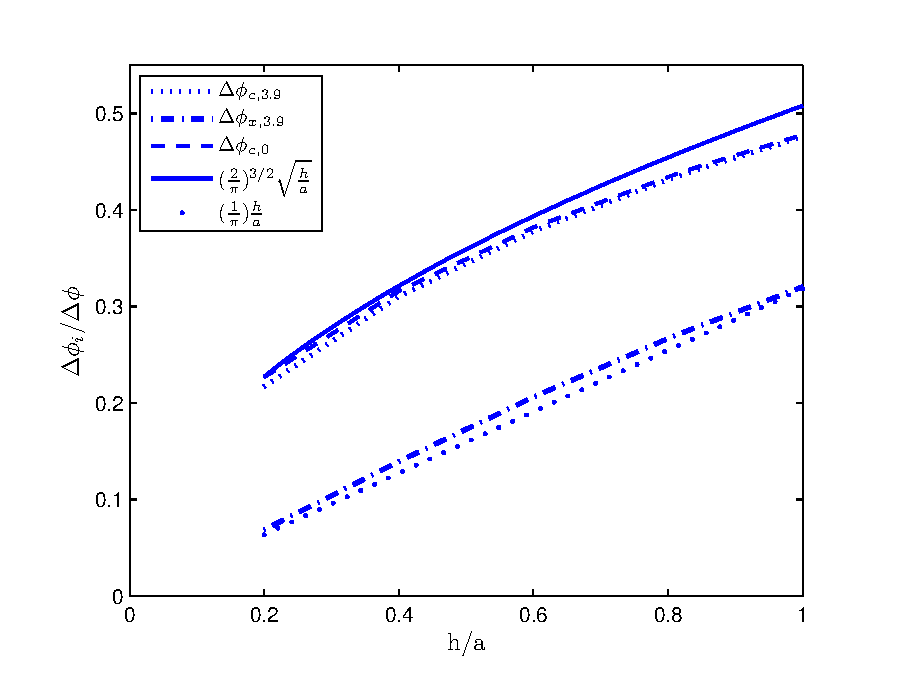
\includegraphics[width=0.7\textwidth,clip=true]{eddies/DeltaV_At_Corner_and_Axis2.eps}
\caption{The potential difference across the cylindrical pore, scaled by the
total potential difference $\Delta\phi$ between the two sides of the
membrane. Potential difference along the pore wall:
Solid line, theoretical prediction
$\Delta\phi_c$
(\ref{delta_phi_c});
dashed line, $\Delta\phi_{c,0}$ computed for $\epsilon_s=0$;
$\cdots$ 
computed for $\epsilon_s/\epsilon_0=3.9$.
Potential difference along the pore axis:
dotted line, $\Delta\phi_{c,3.9}$ 
theoretical prediction $\Delta\phi_x$ (\ref{delta_phi_x});
dash-dotted line, computed $\Delta\phi_{x,3.9}$ for $\epsilon_s/\epsilon_0=3.9$.
\label{fig:DeltaV}}
\end{figure}


\begin{figure}[h]
\centering
\includegraphics[width=0.99\textwidth,clip=true]{eddies/eddy_fig4b.eps}
\caption{Numerically computed streamlines in the neighbourhood of the hole,
$a\kappa=5$, $\epsilon_s/\epsilon_0=3.9$. Uncharged membrane of thickness
(a) $h=0.4a$;
(b) $h=0.8a$;
(c) $h=0.84a$;
(d) $h=a$.
\label{fig:eddies}}
\end{figure}

The set of
time-independent equations governing the electrical potential
$\phi$, the ionic number densities $n^i$,
the fluid velocity $\mathbf{u}$ and fluid pressure $p$
consists of the Poisson equation (\ref{poisson}), the ion
conservation equation (\ref{ion_conservation}) and the Stokes equations
\begin{eqnarray}
-\nabla p + \mu \nabla^2 \mathbf{u} -  \nabla \phi \sum_{i=1}^{N} z_ien^i & = & 0, \label{eq:stokes_eddies}\\
\nabla \cdot \mathbf{u} & = & 0. \label{eq:continuity_eddies}
\end{eqnarray}
We solve the coupled equations (\ref{poisson}), (\ref{ion_conservation}),
(\ref{eq:stokes_eddies}),  and (\ref{eq:continuity_eddies})
by means of a finite volume numerical scheme based upon the
OpenFOAM CFD library \cite{OPENFOAM}.
The surface charge density $\sigma_\text{m}$ in the absence
of any imposed field
is set to zero, and a symmetrical electrolyte
($N=2$, $z_1=-z_2=1$)  is considered, with
identical cationic and anionic mobilities.
There is therefore complete symmetry about the plane of the
membrane, and no net flow through the hole. The relative permittivity
of the electrolyte
is $\epsilon_f/\epsilon_0=80$, where $\epsilon_0$ is the permittivity of
free space, and that of the membrane is set in the computations to be either
$\epsilon_\text{s}/\epsilon_0=3.9$,
corresponding to silica, or $\epsilon_s=0$.
The hole has radius $a=5\rm\ nm$ (a typical
hole size in silica\cite{Keyser2006} or graphene \cite{Garaj2010,Merchant2010}), with
$a\kappa=5$, corresponding to an electrolyte
of strength 95 mM (at 300 K).
The results presented here were performed with a mesh spacing
that varied smoothly from $\kappa^{-1}/10$
close to the membrane and hole, to $\kappa^{-1}$ at the far outer boundary.
The potential difference applied to generate the flow was $\Delta\phi=1\rm\ mV$,
so that $e\Delta\phi/kT\approx 0.04$: fluid velocities are
everywhere proportional
to $(\Delta\phi)^2$ as long as $e\Delta\phi/kT$ is sufficiently small
for the linearized Poisson-Boltzmann equation to be valid, in which case
the streamlines are independent of $\Delta\phi$.
Further details of the computational scheme are given by
Mao et al. \cite{mao2014}.

The difference in
electrical potential between the two ends of the
pore, at the wall of the cylindrical pore, is
$\Delta\phi_c$ (\ref{delta_phi_c}) when $h\ll a$
and this analytic prediction is shown
in Figure \ref{fig:DeltaV}
as a function of $h/a$. We see that the analytic result is in good 
agreement with computed results $\Delta\phi_{c,0}$ ($\epsilon_s=0$)
for $h/a<0.4$.
Also shown are computations for a membrane with relative permittivity
$\epsilon_s/\epsilon_0=3.9$, which differ little from those for
$\epsilon_s/\epsilon_0=0$.
If $h/a$ is sufficiently small, the resistance
of the pore changes only slightly \cite{sherwood2014} from that predicted for
the electric field (\ref{eq:chi_eddies})
when $h=0$.  We therefore expect the current along the
centreline of the pore, well away from the edges,
to be little changed, and the electric field
along the centreline is  still (to a first approximation)
$-\hat{\mathbf{z}}\Delta\phi/(a\pi)$
(\ref{Ez_hole}). The potential difference
between the ends ($z=\pm h/2$) of the pore along the centreline
should therefore be
\begin{equation}
\Delta\phi_x=\frac{\Delta\phi}{\pi}\left(\frac{h}{a}\right),\quad h\ll a.
\label{delta_phi_x}
\end{equation}
This too is shown in Figure \ref{fig:DeltaV}, and we see reasonable agreement
between theory and computation.

\begin{figure}[h]
\centering
\includegraphics[width=0.99\textwidth,clip=true]{eddies/eddy_fig5.eps}
\caption{Schematic showing the boundaries of eddies in Figure \ref{fig:eddies}.
MA and GP represent the membrane surface at $z=h/2$; NC and EQ
the surface at $z=-h/2$. ABC and GFE represent the cylindrical surface of the
nanopore. Stagnation points within fluid (away from the walls)
are at (a) O,D,H, and (b) O,J,K. Axial symmetry implies that
the eddies ABD and GFH in (a) are cross-sections of the same toroidal eddy.
\label{fig:eddy_schematic}}
\end{figure}

When $\epsilon_s/\epsilon_0=3.9$, induced charges
lead to electro-osmosis.
Streamlines computed for the case $h=0.4a$ are shown in
Figure \ref{fig:eddies}(a) and take the form shown schematically in
Figure \ref{fig:eddy_schematic}(a).
Axial symmetry implies that ABD and GFH in Figure \ref{fig:eddy_schematic}(a)
are cross-sections of the same
toroidal eddy (and similarly for CBD and EFH).
However, the eddy pairs ABCD and EFGH in Figure \ref{fig:eddies}(a) are
very small. Flow near the corners A,C,E,G is a combination of the horizontal
velocity (\ref{u_thin_plane}) predicted on the upper and
lower surfaces of the membrane,
and the local corner flow (\ref{u_rho_wedge}), which flows upwards
along BA and FG, thereby causing the horizontal flow to separate at A and G
(and similarly at C and E).  At fixed position, the
uniform flow (\ref{u_thin_plane}) varies as $h^{-1}$, whereas the
corner flow (\ref{u_rho_wedge}) varies as 
$h^{-1/2}$. As $h$ increases, the ratio of the corner flow to horizontal flow
increases, and the eddies become larger, so that the stagnation
points D and H 
(or more correctly, stagnation lines, since the flow has axial symmetry)
move toward the central stagnation point at O.
This is seen in 
Figure \ref{fig:eddies}(b) for  $h=0.8a$.

When $h\approx 0.84a$ the stagnation points D and H merge into O, and
8 eddies meet at O, as seen in Figure \ref{fig:eddies}(c).
Any further increase in $h$ causes the
stagnation point to bifurcate into three points, at O, J and K, as
seen in Figure \ref{fig:eddies}(d) and shown schematically in
Figure \ref{fig:eddy_schematic}(b). Figure \ref{fig:eddies}(c)
shows eddies for $h=0.84a$, and the precise
value for $h$ at which the 8-fold stagnation point is formed lies
within the range $0.83a<h<0.85a$.
Computations with 
larger grid size $\kappa^{-1}/5$ in the vicinity of the membrane gave
streamlines that could not be distinguished from those in Figure
\ref{fig:eddies}, and the 8-fold stagnation point was still formed
at $h\approx 0.84a$,

The Debye length when $h=0.84a$ and $a\kappa=5$
is $\kappa^{-1}=0.238h$. The corner flow discussed in
Section \ref{sec:corner_charge} is valid only outside the charge
cloud (i.e. for $s>\kappa^{-1}$),
in which region the corner flow (\ref{u_s_corner})
is swamped by the velocity (\ref{u_thin_plane})
parallel to the plane of the membrane.
We are therefore unable 
to see in Figure \ref{fig:eddies} regions close to the corners
in which streamlines 
are symmetric about the local coordinate $\theta=0$ (Figure \ref{fig:corner}).

Any asymmetry in the flow caused by a non-zero
surface charge density $\sigma_\text{m}$
or by differences between the mobilities of the ions causes a net flow from
one side of the membrane to the other. If this is weak, the eddies
seen in Figure \ref{fig:eddies} persist, and the net flow has to snake its
way between them, as discussed by Jeffrey and Sherwood \cite{jeffrey1980},
Thamida and Chang \cite{Thamida2002}, and Yossifon {\it et al.}
\cite{yossifon2006}.


\section{Concluding remarks}

We have shown that the system of induced charge electro-osmotic eddies
in a cylindrical pore can have a rich structure that varies markedly
with pore aspect ratio. If flows created by induced charge electroosmosis
are strong
compared to net motion through the pore, there is a danger that
fluid trapped in the eddies may become contaminated (or may degrade)
over time, and lead to contamination of samples passing through the pore.
Such problems can be reduced by suitable choice of
pore geometry and imposed electric field strength, in order to control the
ratio of eddy velocity to volumetric flow rate through the pore.

We thank Professor E. Yariv (Technion) for helpful suggestions.

\chapter{Numerical Simulation of Electroosmosis using OpenFOAM}
\label{chpt:numerical}
\section{Introduction}
In Chapter \ref{chpt:zero_thickness}, \ref{chpt:finite_thickness} and \ref{chpt:eddies}, we introduced numerical simulations of electroosmotic flow in a nanopore system under different conditions. The numerical simulations are carried out using a self-created solver in OpenFOAM. 

\section{PNPStokesFoam - An OpenFOAM solver for PNP-Stokes system of equations in nanopores}
The steady state PNP-Stokes system of equations given in previous chapters are re-written below for completeness of this chapter. 
\begin{eqnarray}
\epsilon \nabla^2 \phi + \sum_{i=1}^{N} z_ien^i & = & 0,
\label{eq:poisson_num}
\\
\nabla\cdot\left\lbrack n^i\mathbf{u} -\omega^i(kT\nabla
n^i + ez_in^i\nabla\phi) \right\rbrack&=&0 ,
\label{eq:NP_num}
\\ 
-\nabla p + \mu \nabla^2 \mathbf{u} -  \nabla \phi \sum_{i=1}^{N} z_ien^i & = & 0, \label{eq:stokes_num}\\
\nabla \cdot \mathbf{u} & = & 0. \label{eq:continuity_num}
\end{eqnarray} 

The set of equations are coupled and need to be solved in an iterative manner. 

OpenFOAM is an open source CFD library \cite{OPENFOAM} designed for computational mechanics. It is based on finite volume method, which we use to discretize the PNP-Stokes equations. OpenFOAM contains a collection of well-designed object-oriented classes to represent mesh, fields, vectors, tensors and matrices, as well as operators on fields and tensors. The discretized matrix equation is solved using the provided OpenFOAM linear solver. OpenFOAM also contains tools for pre-processing and post-processing.

By convention, OpenFOAM solvers are named by ``-Foam''. We hence call our solver PNPStokesFoam. The details of the solvers are explained as follows.

\subsection{The Poisson-Nernst-Planck equations}
\subsubsection{Convection-diffusion equations of ionic species}
Equation \ref{eq:NP_num} is the so-called Nernst-Planck equation for ionic species $n^i$. It is a convection-diffusion equation. Let us first assume the flow field $\mathbf{u}$ and electric field $\phi$ is known. The convective fluxes include the electrophoretic flux $(-\omega^iz_ie\nabla\phi)n^i$ and convective flux $\mathbf{u}n^i$. Finite volume method is used to discretize Equation \ref{eq:NP_num}. Part of the pseudo code is provided to illustrate.

\begin{lstlisting}
surfaceScalarField rhoFluxi    // define electrophoretic velocity
(
	-zi*(Di/kB/T)*e*fvc::snGrad(phiV)*mesh.magSf()
);

ni.boundaryField().updateCoeffs();    // apply boundary condition

fvScalarMatrix niEqn    // assemble matrix equation
(
    fvm::div(rhoFluxi, ni) + fvm::div(phi,ni) - fvm::laplacian(Di, ni)
);  
      
niEqn.relax();    // apply under-relaxation
niEqn.solve();    // solve using provided linear solver
\end{lstlisting}

\textsf{surfaceScalarField} is the name of the class provided by OpenFOAM for a scalar field defined at the control volume faces. An object \textsf{rhoFluxi} of class \textsf{surfaceScalarField} is defined and calculated as the multiplication of electrophoretic velocity $(-\omega^iz_ie\nabla\phi)$ and the control volume face area \textsf{mesh.magSf()}. Here \textsf{fvc::snGrad(phiV)} stands for the explicit finite volume operator of surface normal gradient \textsf{fvc::snGrad} acting on the scalar field \textsf{phiV} ($\phi$). 

Similarly multiplication of convective velocity $\mathbf{u}$ and control volume face area \textsf{mesh.magSf()} gives another object of class \textsf{surfaceScalarField}. We call it \textsf{phi}.

Now we are ready to discretize Equation \ref{eq:NP_num}. An object \textsf{niEqn} of class \textsf{fvScalarMatrix} is defined. This is the linear equation we get from discretization. In line 10, the operator \textsf{fvm::div} is the implicit finite volume operator for $\nabla \cdot$, while the operator \textsf{fvm::laplacian} is the finite volume operator for $\nabla^2$. Line 10 therefore corresponds to Equation \ref{eq:NP_num} in the OpenFOAM syntax.

After the matrix equation has been assembled, under-relaxation is applied (for iteration later), and \textsf{niEqn.solve()} solves this linear equation using the linear solver provided. 

Note that values of \textsf{zi}, \textsf{Di} etc are provided in an OpenFOAM style input file. The finite volume operators are overloaded to work according to user's choice of schemes. Schemes are provided in another input file. For now central difference scheme is used for the Laplacian operator (diffusive term), and second-order upwind scheme is used for divergence operator (convective terms).

The relaxation factor and choice of linear solver can be specified in an input file, too. User can choose different relaxation factors and linear solvers at runtime.

\subsubsection{Electric potential}
We solved Nernst-Planck equation assuming the potential $\phi$ is known. However, $\phi$ needs to be solved from Equation \ref{eq:poisson_num}, which contains $n^i$ at the right hand side. Equation \ref{eq:NP_num} and \ref{eq:poisson_num} are therefore coupled and need to be solved iteratively.

The pseudo code for solving Equation \ref{eq:poisson_num} is illustrated below.

\begin{lstlisting}
solve
(
    -fvm::laplacian(phiV) == e*(z1*n1+z2*n2)/(ep0*epr)    // RHS is the local charge density
);
phiV.relax();    // apply under-relaxation
\end{lstlisting}

Here we assume in total 2 ionic species. The local charge density is calculated explicitly as \textsf{e*(z1*n1+z2*n2)}. This code corresponds to Equation \ref{eq:poisson_num} in an OpenFOAM syntax.


\subsection{Stokes equation}
\subsubsection{Momentum equations}
Once we have a relatively good predict of $n^i$ and $\phi$, we can update the flow field due to electric body force $-e\sum_i(z_in^i)\nabla\phi$. The pseudo code for the momentum equation is illustrated below.

\begin{lstlisting}
fvVectorMatrix UEqn
(
    -fvm::laplacian(mu, U)    // assemble matrix for the momentum equation
);
UEqn.relax();

solve
(
    UEqn == 
	- fvc::grad(p)    // pressure gradient 
	- e*(z1*c1+z2*c2)*fvc::grad(phiV)    //
);
\end{lstlisting}

\textsf{UEqn} is an object of OpenFOAM class \textsf{fvVectorMatrix}. This class is similar to \textsf{fvScalarMatrix} only that it is for a vector equation. Again, operator \textsf{fvm::laplacian} is overloaded to accept different discretization schemes, specified by user at runtime in the input file. The source term for momentum equation includes the pressure gradient, and the electric body force, which is calculated explicitly using the most updated $n^i$ and $\phi$ as \textsf{- e*(z1*c1+z2*c2)*fvc::grad(phiV)}. Here the OpenFOAM operator \textsf{fvc::grad} calculates the gradient of its argument at control volume centers explicitly. This corresponds to Equation \ref{eq:stokes_num} in OpenFOAM syntax.

\subsubsection{SIMPLE algorithm}
Due to the incompressibility of the water, we need to take care of the pressure-velocity coupling. We adopt the SIMPLE algorithm on a collocate grid with the Rhie-Chow interpolation. The pseudo code is illustrated below.

\begin{lstlisting}
volScalarField rAU(1.0/UEqn.A());    // A^{-1}

U = rAU*(UEqn.H() - e*(z1*c1+z2*c2)*fvc::grad(phiV));    // U^*
    
phi = fvc::interpolate(U) & mesh.Sf();    

fvScalarMatrix pEqn
(
    fvm::laplacian(rAU, p) == fvc::div(phi)    // pressure Poisson equation
);
pEqn.setReference(pRefCell, pRefValue);    // set reference value for pressure

pEqn.solve();    // solve pressure equation

phi -= pEqn.flux();
p.relax();
U -= rAU*fvc::grad(p);    // correct velocity field
\end{lstlisting}

The process corresponds to the following algorithm:
\begin{equation}
A \mathbf{U} = \mathbf{H} - \nabla p + \mathbf{f}
\label{eq:SIMPLE1}
\end{equation}
Here $A$ is the diagonal component of matrix \textsf{UEqn}. $\mathbf{H}$ is the off-diagonal terms of the matrix equation. $\mathbf{f}$ stands for body force other than gradient of pressure. In our case it is the electric force. From the momentum equation we have solved for $\mathbf{U}$. However it in general does not satisfy continuity. We use hence use the continuity equation to correct flow field.

From Equation \ref{eq:SIMPLE1} we have 
\begin{equation}
\mathbf{U} = A^{-1}(\mathbf{H}+\mathbf{f}) - A^{-1}\nabla p
\label{eq:SIMPLE2}
\end{equation}
Let us call $A^{-1}(\mathbf{H}+\mathbf{f})$ $\mathbf{U}^*$. If we apply the divergence operator to both sides of Equation \ref{eq:SIMPLE2}, and force $\mathbf{U}$ to satisfy continuity, then we get
\begin{equation}
\nabla \cdot \left(A^{-1}\nabla p\right) = \nabla \cdot \mathbf{U}^*
\label{eq:SIMPLE3}
\end{equation}

From Equation \ref{eq:SIMPLE3} we calculate $p$ and correct the velocity $\mathbf{U}$ to be $\mathbf{U}^* - A^{-1}\nabla p$. This will ensure that the corrected velocity field satisfies continuity.

This algorithm is by nature the SIMPLE algorithm with Rhie-Chow interpolation on a collocated grid. $A^{-1}$ is \textsf{rAU} in the code. Matrix equation \textsf{pEqn} corresponds to Equation \ref{eq:SIMPLE3}.

\subsection{Iteration}
We start from a zero flow field. Equations  (\ref{eq:poisson_num}) and (\ref{eq:NP_num}) are solved sequentially in a loop with under-relaxation until the absolute residual is small. Under--relaxation is necessary because the PNP system is coupled. The electric volume force $- \nabla \phi\sum_i z_ien^i $ is obtained from this solution and used explicitly in the next step: the solution of the incompressible Stokes flow: (\ref{eq:stokes_num}) and (\ref{eq:continuity_num}). The SIMPLE algorithm is used with a fixed volume force density. The flow field is then substituted into (\ref{eq:NP_num}). The PNP equations are then solved again using the updated flow field. An outer loop is constructed to iterate over the PNP loop and Stokes flow module.

\subsection{Boundary conditions}
OpenFOAM provides a collection of built-in boundary conditions such as the Dirichlet boundary condition and the Neumann boundary condition. These boundary conditions can be used in different context for different physical conditions.

A schematic view of the axisymmetric geometry used for the full numerical simulations is provided in Figure \ref{fig:system_num}. 
\begin{figure}[h]
\centering
\includegraphics[width=1.0\textwidth]{openfoam/figure4.eps}
\caption{A typical nanopore geometry of interest}
\label{fig:system_num}
\end{figure}
It consists of a circular hole of radius $a$ in a solid dielectric membrane CDEF of arbitrary thickness $h\ge 0$. The membrane surfaces CD, DE and EF have a uniform surface charge density $\sigma$. Two large cylindrical reservoirs are connected to the pore, one at each end. In our simulation we consider a 1-1 symmetric electrolyte solution containing ions with equal mobilities. Note the length and radius of both the reservoirs are identical, and are $L_R=\max(10a, 10\kappa^{-1})$, chosen to be much larger than either the hole radius $a$ or the Debye length $\kappa^{-1}$  in order to approximate an infinite reservoir. 

We adopt the following boundary conditions \cite{Mao2013}. The ion number densities on AB and GH are constant, and equal to the number density $n_\infty$ in the bulk solution far from any charged surfaces. The electrical potentials are uniform on AB and on GH, with a potential difference of $\Delta\phi$ between the top (AB) and bottom (GH). The pressure $p_{\infty}$ on AB is uniform and equal to that on GH. On the side walls BC and FG, the radial electric field, ionic flux and radial velocity, which decay away from the pore, are set to zero. A zero tangential shear stress is imposed on flow parallel to the side walls. At the membrane surfaces CD, DE and EF, a no--flux condition is used for (\ref{eq:NP}), a no--slip condition for the flow. 

All the boundary conditions mentioned above can be easily implemented using OpenFOAM built-in boundary conditions or 3-rd party boundary condition \textsf{groovyBC}. \textsf{groovyBC} is a 3-rd party extension of OpenFOAM boundary conditions for Robin-type boundary conditions.

The electrostatic boundary condition at membrane surfaces CD, DE and EF needs special treatment.

\subsubsection{Electrostatic boundary condition}
The electric field $\mathbf{E}$ undergoes a jump across the solid membrane-fluid interface such that
$\epsilon \mathbf{E} \cdot  \hat{\mathbf{n}} - \epsilon_{s} \mathbf{E}_{s} \cdot \hat{\mathbf{n}} = \sigma$ 
where $\epsilon$ is the electrical permittivity of the fluid and $\epsilon_{s}$ is the permittivity of the membrane, $\mathbf{E}_{s}$ is the electric field at the interface within the membrane and $\hat{\mathbf{n}}$ is the unit normal at the surface directed into the fluid. The potential $\phi$ is continuous across the interface. 

If the membrane polarizability is sufficiently small that $|\epsilon_{s} \mathbf{E}_{s} \cdot \hat{\mathbf{n}}|\ll|\epsilon \mathbf{E} \cdot  \hat{\mathbf{n}}|$, then the jump condition of the normal component of the field may be replaced by $\epsilon \mathbf{E} \cdot \hat{\mathbf{n}} = \sigma$. This is equivalent to assuming $\epsilon_s$ is 0 (of course this is not physical as no material has relative permittivity less than 1). In this case, the electrostatic boundary condition becomes specifying the normal gradient of $\phi$ at the boundary. This inhomogeneous Neumann boundary condition can be conveniently implemented using OpenFOAM built-in boundary conditions or \textsf{groovyBC}. We have shown in Chapter \ref{chpt:zero_thickness} that assuming $\epsilon_s=0$ has little effect on the total electroosmotic flow through the nanopore when $\sigma \neq 0$. The biggest advantage of applying this assumption is that the computational domain may be restricted to include only the fluid phase.

On the other hand, $|\epsilon_{s} \mathbf{E}_{s} \cdot \hat{\mathbf{n}}$ and $\epsilon \mathbf{E} \cdot  \hat{\mathbf{n}}|$ becomes comparable, such as when $\sigma = 0$, we need the full jump condition of $\mathbf{E}$ as the electrostatic boundary condition. In this case, the flow is due to ICEO effect. We have studied eddies within uncharged nanopores due to ICEO in Chapter \ref{chpt:eddies}. 

On thing to note is that when the full jump condition of $\mathbf{E}$ is used, \textsf{nppStokesFoam} needs to be modified to include the solid membrane region, where the net charge density is 0. Hence, instead of solving Equation \ref{eq:poisson_num} for $\phi$ in the fluid region alone, we need to solve Equation \ref{eq:poisson_num} together with a Laplace equation
\begin{equation}
\epsilon_s \nabla^2 \phi = 0 \qquad within membrane
\label{eq:laplace_num}
\end{equation}
and the coupling condition of $\epsilon \mathbf{E} \cdot  \hat{\mathbf{n}} - \epsilon_{s} \mathbf{E}_{s} \cdot \hat{\mathbf{n}} = \sigma$ at the solid-fluid interface. 

A separate solver \textsf{mrnppStokesFoam} is developed in OpenFOAM to account for this change. \textsf{mr} stands for multi-region. The coupling boundary condition is not provided in standard OpenFOAM in the context of electrostatics. However, OpenFOAM provides a built-in template for thermal boundary condition at the solid-fluid interface in the context of conjugate heat transfer. Due to the similarity of electrostatics and heat conduction, a new OpenFOAM boundary condition is developed using the OpenFOAM template.

The OpenFOAM template relates the value at boundary $T_f$ and the value at the neighboring control volume center $T_c$ (see Figure \ref{fig:CV}) as follows:
\begin{equation}
T_f = f\cdot \mathsf{refValue} + (1-f)\cdot(T_c + \mathsf{refGrad}\cdot\delta)
\label{eq:OF_BC}
\end{equation}
Here $\delta$ is the distance between control volume center and face center, $f$ is a user defined interpolation factor. \textsf{refValue} and \textsf{refGrad} are defined by user to implement different forms of flux-type boundary condition.

\begin{figure}[h]
\centering
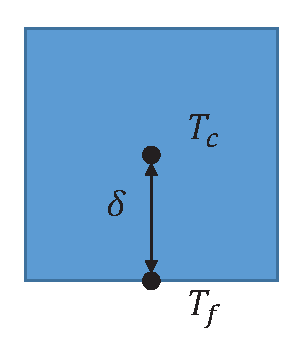
\includegraphics[scale=0.5]{openfoam/CV1.eps}
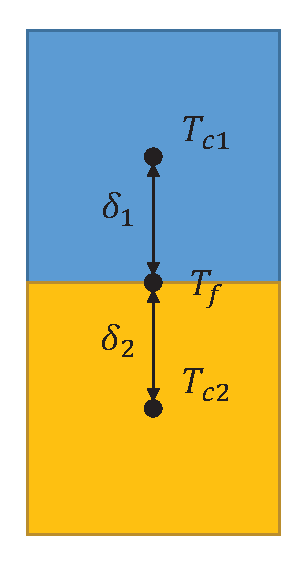
\includegraphics[scale=0.5]{openfoam/CV.eps}
\caption{Control volume (left) adjacent to a boundary and (right) at solid(yellow)-fluid(blue) interface}
\label{fig:CV}
\end{figure}


For a solid-fluid interface shown in Figure \ref{fig:CV}, according to Gauss theorem, we have a discretized form as follows:
\begin{equation}
\epsilon_1 \frac{T_f-T_{c1}}{\delta_1} + \epsilon_2 \frac{T_{c2}-T_f}{\delta_2} = \sigma
\label{eq:OF_BC1}
\end{equation}
Here $\epsilon_1$ and $\epsilon_2$ are permittivity of region 1 and 2, respectively, and $\sigma$ is the surface charge density. Re-arrange Equation \ref{eq:OF_BC1} we get
\begin{equation}
T_f = \left(\frac{\epsilon_1}{\delta_1}+\frac{\epsilon_2}{\delta_2}\right)^{-1} \left( \frac{\epsilon_1}{\delta_1}T_{c1}+\frac{\epsilon_2}{\delta_2}T_{c2}+\sigma\right)
\label{eq:OF_BC2}
\end{equation}

In order to relate $T_{c1}$ and $T_f$, we define $f = \left(\frac{\epsilon_1}{\delta_1}+\frac{\epsilon_2}{\delta_2}\right)^{-1}\frac{\epsilon_2}{\delta_2}$, \textsf{refValue}$=T_{c2}$ and \textsf{refGrad}$=\frac{\sigma}{\epsilon_1}$ in Equation \ref{eq:OF_BC}, we reproduce Equation \ref{eq:OF_BC2}. 

The pseudo code is illustrated below.

\begin{lstlisting}
this->refValue = nbrT;

this->refGrad = surfCharge / myEps;

this->f = nbrKDelta / (nbrKDelta + myKDelta);
\end{lstlisting}
For control volume 1, control volume 2 is its neighbor across the interface, hence $T_{c2}$ is \textsf{nbrT} in the code. Intuitively, $\epsilon_1$ is \textsf{myEps}, $\sigma/\delta$ is called \textsf{KDelta} in the code, and $\sigma$ \textsf{surfCharge}.

For control volume 2, the same self-neighbor relation holds. The code does not need to be modified.

\section{Concluding remarks}
We have used the OpenFOAM CFD library to develop solvers for PNP-Stokes equations. Finite volume method is used to discretize the governing equations. The discretized equations are then solved iteratively due to multiphysics coupling and velocity-pressure coupling. These solvers have been applied successfully to simulations of nanopore problems described in previous chapters. Both qualitative and quantitative agreements have been reached.

OpenFOAM provides templates for solvers and boundary conditions. These templates are modified by the author to create new solvers and boundary conditions suitable for the problems of interest. For instance, the jump condition of the electric field at solid-fluid interface is created in analogous to OpenFOAM thermal boundary condition in conjugate heat transfer problems. In addition, OpenFOAM has large collections of third-party extension due to its popularity in the CFD community. We have used the \textsf{groovyBC} (part of the \textsf{swak4Foam} extension) created by Dr. Bernhard Gschaider. Here we thank the OpenFOAM community for sharing these powerful tools. 

The author also thanks Dr. Neelesh Patankar for helpful guidance and discussions on finite volume method and CFD.

\chapter{Conclusion}
In the current work, electroosmotic flow in a single nanopore under an applied electric field is studied both theoretically and numerically. Different scenarios have been considered, including the case when pore thickness is 0 or finite, and the case when the membrane surface charge density is finite or 0. A net flow exists when surface charge density is nonzero, and the flow rate is computed both from the reciprocal theorem and numerical simulations. Eddies form with the nanopore due to ICEO when membrane surface is uncharged. The shape of the eddies are predicted by numerical simulations.

If the membrane surfaces have intrinsic surface charges, under the assumption of weak field in the Debye-H\"{}uckel limit, asymptotic analysis is carried out and it is shown that the net electric force acting on the fluid is $\rho_0\nabla\chi$, where $\rho_0$ is the local charge density at equilibrium (induced by intrinsic surface charge on the membrane), and $\chi$ is the Ohmic potential. Physically this result means the driving force of the fluid flow is the Ohmic potential field acting on the equilibrium charge cloud, and that the charge cloud is not disturbed by either the external electric field or the induced electroosmostic flow. By utilizing the reciprocal theorem, we show the volumetric flow rate can be expressed as an integral, without solving the detailed flow field. For a circular hole on a zero-thickness membrane, the building blocks of the integral are available theoretically. The integral is then expressed in closed form and computed up to quadrature. The result agrees with full numerical simulation of the PNP-Stokes equations. The ratio of volumetric flow rate to the applied voltage is defined as ``electroosmotic access resistance'' in analogy to its counterpart in electrostatics.

When the nanopore is circular but has non-zero thickness (cylindrical), we patch the solution of electroosmosis through a zero-thickness pore with the classic theory of electroosmosis in a cylinder. The patched solution gives a total electroosmotic conductance as a weighed average of the electroosmotic conductance of a circular hole, and the electroosmotic conductance of a cylinder. The solution agrees with numerical simulation except at the thick Debye length limit $a\kappa \gg 1$. We show that the reason is that the charge overspill from the pore to outside (and vice versa) are significant when Debye layer is thick. Under this circumstance the electroosmotic conductances for both a hole and a cylinder need to be corrected. We theoretically provide such corrections, and the modified solution agrees with numerical simulation.

When the membrane surfaces do not have surface charges, the problem has symmetry such that no net flow will be generated through the nanopore. This does not mean no flow at all. Instead ICEO effects can generate toroidal eddies within the nanopore. We provide theoretical analysis for this problem in the linear regime. Far away from the edge of the hole, the induced zeta potential is worked out based on the assumption that the radial variations can be neglected. Using the solution of the Laplace equation to calculate the tangential electric field, the Smoluchowski velocity is subsequently obtained. This is used as the outer solution, and its inner limit (towards the edge of the hole) is matched with a local solution of the iceo problem. The local solution is worked out in 3 steps. First, the method of conformal mapping is used to obtain the Ohmic potential outside the Debye layer and within the solid wedge. Then we follow Thamida and Chang \cite{Thamida2002} and work out the induced zeta potential. Finally the Smoluchowski velocity is presented. We also use full numerical simulations to show that the shape of the toroidal eddies on the geometry of the pore. The interesting topology of vortex pairs form within the nanopore, and one particular interesting case is when the eddies meet at one single stagnation point, dividing the fluid domain into 8 separate regions.

Finally, the PNP-Stokes solvers are introduced. These solvers are based on finite volume method using the OpenFOAM CFD library. The equations are solved iteratively due to the multiphysics coupling. When the polarizability of the solid membrane can be neglected, the jump condition of electric field at the solid-fluid membrane reduces to a Neumann boundary condition, and the computation can be restricted to the fluid region alone. When the polarizability of the solid membrane needs to be taken into account, the potential in the solid region needs to be computed as well, and specific solver and boundary condition are developed to account for this additional multi-region coupling.

% The command \includeonly above allows to include a selected 
% set of chapters only.

% (The following suggested by Francisco Iacobelli - 5/11/2010)
% In case, you want to use BibTeX, you should replace (or comment)
% the bibliography environment.
% Instead uncomment the following 3 lines and replace <bib file>
% with your .bib file:
%\renewcommand\refname{\begin{centering}References\end{centering}}
\bibliography{references}
\bibliographystyle{unsrt} %or another suitable style.

%\appendix		% Appendix begins here (optional).
%
%%\appendices	        % If more than one appendix chapters,
%				% use appendices instead of appendix
%
%\chapter{Title of Appendix}	% First appendix chapter, i.e., Appendix A.
%
%\section{First section of Appendix}	% This is appendix section 1.
%
%This is the Appendix.
%
\end{document}

